% Options for packages loaded elsewhere
% Options for packages loaded elsewhere
\PassOptionsToPackage{unicode}{hyperref}
\PassOptionsToPackage{hyphens}{url}
\PassOptionsToPackage{dvipsnames,svgnames,x11names}{xcolor}
%
\documentclass[
  letterpaper,
  DIV=11,
  numbers=noendperiod]{scrartcl}
\usepackage{xcolor}
\usepackage{amsmath,amssymb}
\setcounter{secnumdepth}{-\maxdimen} % remove section numbering
\usepackage{iftex}
\ifPDFTeX
  \usepackage[T1]{fontenc}
  \usepackage[utf8]{inputenc}
  \usepackage{textcomp} % provide euro and other symbols
\else % if luatex or xetex
  \usepackage{unicode-math} % this also loads fontspec
  \defaultfontfeatures{Scale=MatchLowercase}
  \defaultfontfeatures[\rmfamily]{Ligatures=TeX,Scale=1}
\fi
\usepackage{lmodern}
\ifPDFTeX\else
  % xetex/luatex font selection
\fi
% Use upquote if available, for straight quotes in verbatim environments
\IfFileExists{upquote.sty}{\usepackage{upquote}}{}
\IfFileExists{microtype.sty}{% use microtype if available
  \usepackage[]{microtype}
  \UseMicrotypeSet[protrusion]{basicmath} % disable protrusion for tt fonts
}{}
\makeatletter
\@ifundefined{KOMAClassName}{% if non-KOMA class
  \IfFileExists{parskip.sty}{%
    \usepackage{parskip}
  }{% else
    \setlength{\parindent}{0pt}
    \setlength{\parskip}{6pt plus 2pt minus 1pt}}
}{% if KOMA class
  \KOMAoptions{parskip=half}}
\makeatother
% Make \paragraph and \subparagraph free-standing
\makeatletter
\ifx\paragraph\undefined\else
  \let\oldparagraph\paragraph
  \renewcommand{\paragraph}{
    \@ifstar
      \xxxParagraphStar
      \xxxParagraphNoStar
  }
  \newcommand{\xxxParagraphStar}[1]{\oldparagraph*{#1}\mbox{}}
  \newcommand{\xxxParagraphNoStar}[1]{\oldparagraph{#1}\mbox{}}
\fi
\ifx\subparagraph\undefined\else
  \let\oldsubparagraph\subparagraph
  \renewcommand{\subparagraph}{
    \@ifstar
      \xxxSubParagraphStar
      \xxxSubParagraphNoStar
  }
  \newcommand{\xxxSubParagraphStar}[1]{\oldsubparagraph*{#1}\mbox{}}
  \newcommand{\xxxSubParagraphNoStar}[1]{\oldsubparagraph{#1}\mbox{}}
\fi
\makeatother


\usepackage{longtable,booktabs,array}
\usepackage{calc} % for calculating minipage widths
% Correct order of tables after \paragraph or \subparagraph
\usepackage{etoolbox}
\makeatletter
\patchcmd\longtable{\par}{\if@noskipsec\mbox{}\fi\par}{}{}
\makeatother
% Allow footnotes in longtable head/foot
\IfFileExists{footnotehyper.sty}{\usepackage{footnotehyper}}{\usepackage{footnote}}
\makesavenoteenv{longtable}
\usepackage{graphicx}
\makeatletter
\newsavebox\pandoc@box
\newcommand*\pandocbounded[1]{% scales image to fit in text height/width
  \sbox\pandoc@box{#1}%
  \Gscale@div\@tempa{\textheight}{\dimexpr\ht\pandoc@box+\dp\pandoc@box\relax}%
  \Gscale@div\@tempb{\linewidth}{\wd\pandoc@box}%
  \ifdim\@tempb\p@<\@tempa\p@\let\@tempa\@tempb\fi% select the smaller of both
  \ifdim\@tempa\p@<\p@\scalebox{\@tempa}{\usebox\pandoc@box}%
  \else\usebox{\pandoc@box}%
  \fi%
}
% Set default figure placement to htbp
\def\fps@figure{htbp}
\makeatother


% definitions for citeproc citations
\NewDocumentCommand\citeproctext{}{}
\NewDocumentCommand\citeproc{mm}{%
  \begingroup\def\citeproctext{#2}\cite{#1}\endgroup}
\makeatletter
 % allow citations to break across lines
 \let\@cite@ofmt\@firstofone
 % avoid brackets around text for \cite:
 \def\@biblabel#1{}
 \def\@cite#1#2{{#1\if@tempswa , #2\fi}}
\makeatother
\newlength{\cslhangindent}
\setlength{\cslhangindent}{1.5em}
\newlength{\csllabelwidth}
\setlength{\csllabelwidth}{3em}
\newenvironment{CSLReferences}[2] % #1 hanging-indent, #2 entry-spacing
 {\begin{list}{}{%
  \setlength{\itemindent}{0pt}
  \setlength{\leftmargin}{0pt}
  \setlength{\parsep}{0pt}
  % turn on hanging indent if param 1 is 1
  \ifodd #1
   \setlength{\leftmargin}{\cslhangindent}
   \setlength{\itemindent}{-1\cslhangindent}
  \fi
  % set entry spacing
  \setlength{\itemsep}{#2\baselineskip}}}
 {\end{list}}
\usepackage{calc}
\newcommand{\CSLBlock}[1]{\hfill\break\parbox[t]{\linewidth}{\strut\ignorespaces#1\strut}}
\newcommand{\CSLLeftMargin}[1]{\parbox[t]{\csllabelwidth}{\strut#1\strut}}
\newcommand{\CSLRightInline}[1]{\parbox[t]{\linewidth - \csllabelwidth}{\strut#1\strut}}
\newcommand{\CSLIndent}[1]{\hspace{\cslhangindent}#1}



\setlength{\emergencystretch}{3em} % prevent overfull lines

\providecommand{\tightlist}{%
  \setlength{\itemsep}{0pt}\setlength{\parskip}{0pt}}



 


\KOMAoption{captions}{tableheading}
\usepackage{tikz}
\usepackage{pgfplots}
\usepackage{amsmath}
\usepackage{relsize}
\usepackage{relsize,exscale}
\usepackage[straightvoltages]{circuitikz}
\usepackage{braket}
\usepackage{mathtools}
\makeatletter
\@ifpackageloaded{caption}{}{\usepackage{caption}}
\AtBeginDocument{%
\ifdefined\contentsname
  \renewcommand*\contentsname{Table of contents}
\else
  \newcommand\contentsname{Table of contents}
\fi
\ifdefined\listfigurename
  \renewcommand*\listfigurename{List of Figures}
\else
  \newcommand\listfigurename{List of Figures}
\fi
\ifdefined\listtablename
  \renewcommand*\listtablename{List of Tables}
\else
  \newcommand\listtablename{List of Tables}
\fi
\ifdefined\figurename
  \renewcommand*\figurename{Figure}
\else
  \newcommand\figurename{Figure}
\fi
\ifdefined\tablename
  \renewcommand*\tablename{Table}
\else
  \newcommand\tablename{Table}
\fi
}
\@ifpackageloaded{float}{}{\usepackage{float}}
\floatstyle{ruled}
\@ifundefined{c@chapter}{\newfloat{codelisting}{h}{lop}}{\newfloat{codelisting}{h}{lop}[chapter]}
\floatname{codelisting}{Listing}
\newcommand*\listoflistings{\listof{codelisting}{List of Listings}}
\makeatother
\makeatletter
\makeatother
\makeatletter
\@ifpackageloaded{caption}{}{\usepackage{caption}}
\@ifpackageloaded{subcaption}{}{\usepackage{subcaption}}
\makeatother
\usepackage{bookmark}
\IfFileExists{xurl.sty}{\usepackage{xurl}}{} % add URL line breaks if available
\urlstyle{same}
\hypersetup{
  pdftitle={Introduction à la théorie quantique - version avec corrigé des exercices},
  pdfauthor={Stéphane Caporali},
  colorlinks=true,
  linkcolor={blue},
  filecolor={Maroon},
  citecolor={Blue},
  urlcolor={Blue},
  pdfcreator={LaTeX via pandoc}}


\title{Introduction à la théorie quantique - version avec corrigé des
exercices}
\author{Stéphane Caporali}
\date{2025-08-29}
\begin{document}
\maketitle

\renewcommand*\contentsname{Table of contents}
{
\hypersetup{linkcolor=}
\setcounter{tocdepth}{3}
\tableofcontents
}

\section{1. Démarche pédagogique :}\label{duxe9marche-puxe9dagogique}

Depuis l'enseignement de la quantique il y a 40 ans oú l'objectif était,
pour un futur ingénieur, d'acquérir une compétence dans les
semi-conducteurs, est apparu une ``seconde révolution'' quantique portée
notamment par la vérification expérimentale de l'intrication, ouvrant la
porte à l'\emph{informatique quantique}. L'objectif pour le futur
ingénieur est d'être sensibilisé aux enjeux industriels d'aujourd'hui.
Bien que ne s'adressant pas directement à de futur physiciens il est
décidé de ne pas trop tomber dans la simplification, l'approche de ce
cours est intuitive mais rigoureuse.

On lit fréquemment dans les livres pédagogiques récents que l'on aborde
les choses par la mécanique ondulatoire et que l'on aurait pu tout aussi
bien utiliser la mécanique matricielle. Toutefois j'ai découvert un jour
en fouillant dans une bibliothèque universitaire le livre : ``Calcul
matriciel. Application à la physique quantique'' (Blaquière and Jean
1960) qui propose une approche par la mécanique matricielle. J'ai trouvé
cette démarche audacieuse d'autant plus qu'il est utilisé le moins de
mathématiques possibles ce qui rend le livre accessible. L'idée de
départ de ce cours a été d'aller le plus loin possible de cette façon là
et de ne commencer à parler d'onde que lorsque cela devient vraiment
nécessaire. En publiant son livre en 1960, Augustin Blaquière
s'adressait plus particulièrement aux élèves des classes de
mathématiques supérieures et mathématiques spéciales ainsi qu'aux
étudiants des facultés, et à certains ingénieurs. Ensuite une montée en
rigueur se fait grace à l'ouvrage recent : (Wiggins 2024). En effet
celui ci s'adresse a des mathématiciens et la physique quantique c'est
comme la haute montagne on ne peut pas compter que sur sa jujotte et son
bon sens. Il faut rentrer dans l'outil mathématique sinon on ne peut
rien faire. Il faut accepter l'esprit du débutant afin de se laisser
guider par une rigueur moins naturelle mais nécessaire.

Il s'agit aussi de démythifier la physique quantique. On entend dire que
par rapport au monde classique le monde quantique serait quelque chose
complètement contre-intuitif. Il y a la fameuse phrase de Feyman qui dit
que personne ne comprend la physique quantique et que l'on sort souvent
de son contexte. En réalité des exemples pris dans le domaine de
l'acoustique ou de électronique donnent pas mal de clés. De plus, les
notions d'algèbre linéaire sont amenées de façon très progressive pour
permettre à des gens qui ne sont pas sensibilisés d'y rentrer.

Veuillez noter que ce cours nécessite des connaissances préalables en
physique des ondes et concernant les équations différentielles.
Toutefois quelques rappels sont insérés dans le cours. Ce cours
s'accompagne d'exercices essentiellements issus du livre d'Hamid Najib
(Najib 2022) fruit d'une expérience d'enseignement de l'auteur.

Ne sont pas traités dans ce cours :

\begin{enumerate}
\def\labelenumi{\arabic{enumi}.}
\item
  Le modèle de Bohr
\item
  L'oscillateur harmonique
\item
  Concernant le puits de potentiel on reste sur le puits de potentiel
  infini.
\end{enumerate}

Une attention particulière est accordée à l'onde de De Broglie, au
principe d'incertitude d'Heisenberg ainsi qu'aux portes logiques
quantiques, et au lien avec \emph{le domaine des réseaux en général et à
la blockchain en particulier}.

\section{2. Introduction historique}\label{introduction-historique}

On situe quelquefois la naissance de la quantique par la decouverte de
la constante de planck, ou bien celle de l equation de Schrodinger, ou
bien le papier de Heisenberg de 1925 qui pose un formalisme dans le
document.

\pandocbounded{\includegraphics[keepaspectratio]{Article_1925.png}}

Ainsi historiquement, avant d'etre l'homme des matrices ou du principe
d'incertitude, Heisenberg s'est interesse aux series de fourier.

Ainsi Heisenberg a imagine un tableau metant en correspondance les
niveaux n et n+1 de le'enrgie. Chaque ligne correspond au developpement
en serie de fourier d'une fonction, par exemple la fonction position.
Ainsi une case peut etre vue comme une composante de la serie de
fourier, On ne parle pas encore de matrice et ni d'espace vectoriel.

Toutefois Heisenberg a la bonne idee de chercher a mettre l'expression
sous la forme d'un devellopement de degre 2. En effet l'energie
s'exprime au carre et si l'amplitude des series de fourier represente un
carre alors il s'agit peur etre d'un resultat observable.

ainsi on trouve dans le document (Heisenberg 1925) l'expression suivante
exprimee ici dans le formalisem de la physique classque mais l'idee y
est :

\begin{itemize}
\tightlist
\item
  tout d'abord, nous cherchons a exprimer la position x d'une particule.
  En supossons la fonction periodique nous allons la decomposer en serie
  de fourier,
\end{itemize}

\begin{quote}
\(x=\Sigma_{+\infty}^{-\infty}a_{\alpha}(n)e^{i\alpha\omega_{n}t}\) dann
ist
\end{quote}

Il suffit de la deriver pour prendre l'expression de v.

\begin{quote}
\(m\dot{x}=\Sigma_{+\infty}^{-\infty}a_{\alpha}(n)i\alpha\omega_{n}e^{i\alpha\omega_{n}t}\)
und
\end{quote}

Heisenger s'interesse a la notion d'action, prise comme l'impact et qui
peut s'exprimer comme une energie que multiplie une duree, ou comme une
vitesse que multiplie une distance. H signifie deja le quantum d'action.

\begin{quote}
\(\oint pdq=\oint m\dot{x}dx=J(=nh)\)
\end{quote}

En basculant de dq en dt on introduit un carre. L'energie cinetique est
une vitesse au carree. Le carre introduit qu'il s'agit d'une energie. Le
terme \(a\) lie a l'amplitude se retourve deux fois.

\begin{quote}
\(\oint m\dot{x}dx=\oint m\dot{x}^2dt=2\pi m\Sigma_{+\infty}^{-\infty}a_{\alpha}(n)a_{-\alpha}(n)\alpha^2\omega_{n}\)
\end{quote}

\begin{quote}
Da ferner \(a_{\alpha}(n)=\overline{a_{\alpha}(n)}\) is\textasciitilde{}
(x soll reeli sein), so folgt
\end{quote}

\begin{quote}
\(\oint mx^2dt=2\pi \Sigma_{+\infty}^{-\infty} |a_{\alpha}(n)|^2\alpha^2\omega_{n}\)
\end{quote}

\begin{quote}
Dieses Phasenintegral hat man bisher meist; gleieh einem ganzen
Vielfachen yon h, also glelch n.~h gesetzt; eiae solche Bedingung fiigt
sich aber nJcht nur sehr gezwungen der mechanischen Rechnung ein, sie
erscheint auch selbst yore bisherigen Standpunkt aus Jm Sinne des
Korrespondenzprinzips willktirlieh; denn korrespondenzmal3ig sind die J
nur bis auf eine additive Konst\textasciitilde nte als ganzzahtige
Viel\textasciitilde ache von l\textasciitilde{} festgelegt, und an
Stelle yon (14) hatte naturgemalJ zu treten:
\end{quote}

Ici Heisenberg expliaue que cette formulation ne le satisfait pas. Ici
en prefere une autre :

\begin{quote}
\(\frac{d}{dn}(nh)=\frac{d}{dn}\oint m\dot{x}dt\) das heist
\end{quote}

\begin{quote}
\(h=2\pi m \Sigma_{+\infty}^{-\infty} \alpha \frac{d}{dn} a\alpha \omega_{n} |a_{\alpha}|^2\)
\end{quote}

Il faut voir que ce qui interesse Heisenberg c'est l'amplitude a qu'on
peut associer a chacun des composantes des series de fourier, De plus
ici on s'exprime en utilisant un formalisme classique et Heisenberg avec
ses tableaux propose l'amorce d'un cadre conceptuel qui precede les
matrices.

Il s'agit simplement d'une esquise d'interpretation qui ne se substitue
pas a une travail d'historien mais a pour objectif d'etre un paragrphae
introductif.

\begin{figure}[H]

{\centering \includegraphics[width=5.20833in,height=\textheight,keepaspectratio]{Schemas/Solvay_conference_1927.jpg}

}

\caption{Cinquième Congrès Solvay de physique, 1927. Source : Wikipedia}

\end{figure}%

Heisenberg avait 24 ans et aps encore sa these. Mais il faut voir que la
theorie quantique a bien connece par des choses petites et les
developpement mathematiques sont arrives rapidement derriere. Lors du
coingre Solvay de 1927 trois ans plus tard (figure 1) la dynamique etait
en marche et aboutira de facom plus ou noins direct au consensus de
copenhague.

\section{2. Faits experimentaux :}\label{faits-experimentaux}

\subsection{2.1 Le corps noir :}\label{le-corps-noir}

Le corps noir n'est pas forcement noir. Il s'agit d'une cavité avec une
ouverture qui piège les rayons lumineux à l' intérieur de la cavité. La
cavité ne peut pas émettre les rayons reçus, toutefois elle se réchauffe
(et donc émet de l' énergie) mais sans émission de lumière. Elle se
comporte comme si elle était noire. L'émission d'énergie sous forme de
chaleur suit une courbe qui n'est pas explicable par la physique
classique.

\usetikzlibrary{arrows}
\begin{figure}
\centering
    
 
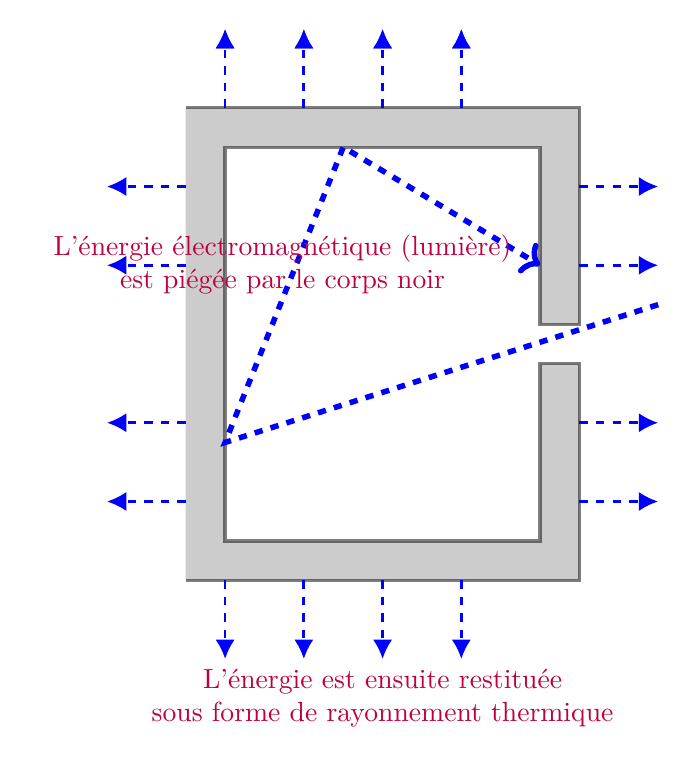
\begin{tikzpicture}[scale=0.5]
  \fill [fill=black!40, draw=black, very thick, semitransparent]  
  (0,0) 
    -- (10,0) 
    -- (10,5.5) 
    -- (9,5.5) 
    -- (9,1)
    -- (1,1)
    -- (1,11)
    -- (9,11)
    -- (9,6.5)
    -- (10,6.5)
    -- (10,12)
    -- (0,12) ;
 \draw[->, magenta,line width=2pt] (12,7) -- (1,3.5) -- (4,11) -- (9,8) [dashed, blue] node[left, purple] {\begin{tabular}{c}L’énergie électromagnétique (lumière) \\ est piégée par le corps noir\end{tabular}};

 \draw [arrows = {-Latex[width=7pt, length=7pt]},dashed, blue,line width=1pt] (10,2) -- (12,2);
 \draw [arrows = {-Latex[width=7pt, length=7pt]},dashed, blue,line width=1pt] (10,4) -- (12,4);
 \draw [arrows = {-Latex[width=7pt, length=7pt]},dashed, blue,line width=1pt] (10,8) -- (12,8);
 \draw [arrows = {-Latex[width=7pt, length=7pt]},dashed, blue,line width=1pt] (10,10) -- (12,10);

\draw [arrows = {-Latex[width=7pt, length=7pt]},dashed, blue,line width=1pt] (0,2) -- (-2,2);
 \draw [arrows = {-Latex[width=7pt, length=7pt]},dashed, blue,line width=1pt] (0,4) -- (-2,4);
 \draw [arrows = {-Latex[width=7pt, length=7pt]},dashed, blue,line width=1pt] (0,8) -- (-2,8);
 \draw [arrows = {-Latex[width=7pt, length=7pt]},dashed, blue,line width=1pt] (0,10) -- (-2,10);

\draw [arrows = {-Latex[width=7pt, length=7pt]},dashed, blue,line width=1pt] (1,12) -- (1,14);
 \draw [arrows = {-Latex[width=7pt, length=7pt]},dashed, blue,line width=1pt] 
 (3,12) -- (3,14);
 \draw [arrows = {-Latex[width=7pt, length=7pt]},dashed, blue,line width=1pt] (5,12) -- (5,14);
 \draw [arrows = {-Latex[width=7pt, length=7pt]},dashed, blue,line width=1pt] (7,12) -- (7,14);

 \draw [arrows = {-Latex[width=7pt, length=7pt]},dashed, blue,line width=1pt] (1,12) -- (1,14);
 \draw [arrows = {-Latex[width=7pt, length=7pt]},dashed, blue,line width=1pt] 
 (3,12) -- (3,14);
 \draw [arrows = {-Latex[width=7pt, length=7pt]},dashed, blue,line width=1pt] (5,12) -- (5,14);
 \draw [arrows = {-Latex[width=7pt, length=7pt]},dashed, blue,line width=1pt] (7,12) -- (7,14);

 \draw [arrows = {-Latex[width=7pt, length=7pt]},dashed, blue,line width=1pt] (1,0) -- (1,-2);
 \draw [arrows = {-Latex[width=7pt, length=7pt]},dashed, blue,line width=1pt] 
 (3,0) -- (3,-2);
 \draw [arrows = {-Latex[width=7pt, length=7pt]},dashed, blue,line width=1pt] (5,0) -- (5,-2);
 \draw [arrows = {-Latex[width=7pt, length=7pt]},dashed, blue,line width=1pt] (7,0) -- (7,-2);
 \draw (5,-3) node [purple] {\begin{tabular}{c}L’énergie est ensuite restituée \\ sous forme de rayonnement thermique\end{tabular}};

       
\end{tikzpicture}
       
 
\caption{Certains objets, comme l'intérieur d'un four chauffé uniformément, peuvent approcher le modèle du corps noir.}
\end{figure}

A un moment Planck eut l'idée d'introduire une constante h qui règle le
problème qui vaut : \(h=6,626.10^{-34}J.s\). Il imaginait que le corps
noir se comportait comme un oscillateur harmonique de fréquence \(\mu\)
mais dont les niveaux énergie sont quantifiés. Il s'agissait d'une
astuce afin de faire coller les résultats avec l'expérience. Planck ne
prévoyait pas un très grand avenir scientifique à la constante \(h\)
qu'il avait introduite. C'est Einstein qui valorisa cette constante en
proposant en 1905 une interprétation simple et efficace de l'effet
photoélectrique en postulant que le rayonnement électromagnétique était
lui même composé de quantas de lumière, appelés plus tard photons
d'énergie \(\epsilon=h\mu\). Ces quantas d' énergie ne furent appelées
photons qu'en 1926.

\begin{figure}[H]

{\centering \includegraphics[width=4.16667in,height=\textheight,keepaspectratio]{Schemas/Corps.png}

}

\caption{Courbes de rayonnement du corps noir à différentes températures
selon l'équation de Planck (courbes en couleur) comparées à une courbe
établie selon la théorie classique de Rayleigh-Jeans (courbe en noir).
Source : wikipedia}

\end{figure}%

Max Planck (Planck 1901) écrit :

\begin{quote}
``si nous appliquons la loi de déplacement de Wien sous sa dernière
forme à l'expression de l'entropie S, nous nous rendons compte que
l'élément d'énergie \(\epsilon\) doit être proportionnel au nombre
d'oscillations \(\mu\) et que donc : \(\epsilon=h\mu\)''
\end{quote}

puis un peu plus loin Planck donne une première estimation pour \(h\) :

\begin{quote}
\(h=6.55.10^{-27} erg.sec\)
\end{quote}

A comparer avec la valeur réelle : \(6,62607015 \times 10^{-34} J.s\)

\(h\) s'exprime en joules secondes : en physique il s'agit d'une action.
Pour cette raison on appelle aussi \(h\) le quantum d'action.

\subsection{2.2 L'effet photoélectrique
:}\label{leffet-photouxe9lectrique}

Albert Einstein écrit : (Einstein 1905)

\begin{quote}
``Il me semble que les observations portant sur le''rayonnement noir''
(\ldots) apparaissent comme plus compréhensibles si on admet que
l'energie de la lumière est distribuée de façon discontinue dans
l'espace. Selon l'hypothèse envisagée ici, lors de la propagation d'un
rayon lumineux émis par une source ponctuelle, l'énergie n'est pas
distribuée de façon continue sur des espaces de plus en plus grands,
mais est constituée d'un nombre fini de quantas d'énergie localises en
des points de l'espace''.
\end{quote}

Einstein pose dans cet article daté du 09 juin 1905 (soit environ 6 mois
avant son célèbre article sur la relation masse énergie) la
discontinuité de l'énergie non plus comme une constatation expérimentale
mais comme un fondement théorique. Cet article lui vaudra le Prix Nobel
de physique en 1921.

\usetikzlibrary {arrows.meta}
\usetikzlibrary {decorations.pathmorphing}
\begin{figure} 
\centering
 
     
 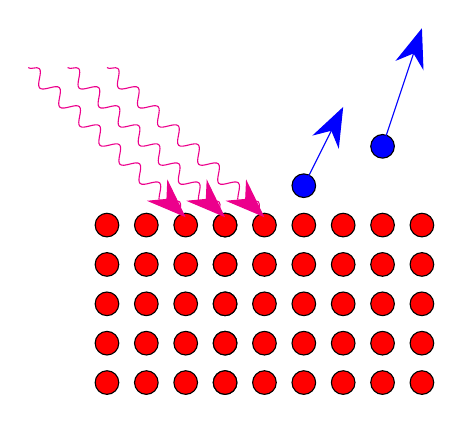
\begin{tikzpicture}[scale=0.5]

 %   \tikzset{shift={(current page.center)},yshift=-1.5cm}
  
  \foreach \x in {-5,-4,-3,-2,-1,-2,0,1,2,3}
    \foreach \y in {-1,0,1,2,3}
      {
        \draw [fill=red] (\x,\y) circle (0.3cm);
      %  \fill (\x,\y) circle (0.1cm);
      }

 %   \draw[decorate,decoration={snake,segment length=2cm},->] (0,0) - - (10,0);
    \draw[decorate,decoration=snake,magenta,-{Stealth[length=5mm]}] (-5,7) - - (-1,3.2) ;
    \draw[decorate,decoration=snake,magenta,-{Stealth[length=5mm]}] (-6,7) - - (-2,3.2) ;
    \draw[decorate,decoration=snake,magenta,-{Stealth[length=5mm]}] (-7,7) - - (-3,3.2) ;

    
    \draw [fill=blue] (2,5) circle (0.3cm);
    \draw[blue,-{Stealth[length=5mm]}] (2,5) -- (3,8);

     \draw [fill=blue] (0,4) circle (0.3cm);
    \draw[blue,-{Stealth[length=5mm]}] (0,4) -- (1,6);
    
   % \draw[decorate,decoration=snake ] (0,0) arc (0:180:3 and 2);

   
   
\end{tikzpicture}

\caption{ L'énergie reçue par le rayonnement électromagnétique va permettre à des électrons de s'éjecter du matériau. On observe une corrélation entre l'énergie reçue (quantifiée) et celle de l'électron}
\end{figure}

L'équation d'Einstein pour l'effet photoélectrique s'écrit :

\[ \boxed{h\nu =W_{S}+{\frac {1}{2}}mv^{2}}\] où :

\(h\nu\) est l'énergie du photon ;

\(W_{S}\) est l'énergie de liaison de l'électron ;

\(\frac {1}{2}mv^{2}\) est l'énergie cinétique finale de l'électron.
L'énergie d'un photon est caractérisée par la formule.

\emph{On considère que l'effet photoélectrique a fait apparaître
l'aspect corpusculaire de la lumière (en plus de ondulatoire). (Greiner
2009)}

\subsection{4. Expérience des fentes d'Young
:}\label{expuxe9rience-des-fentes-dyoung}

\subsubsection{4.1 Fentes d'Young avec la lumière
:}\label{fentes-dyoung-avec-la-lumiuxe8re}

En optique on admet que les trous S1 et S2 se comportent comme des
sources secondaires qui, issues de la même source primaire S, mettent de
sondes sphériques cohérentes entre elles. C'est le principe
d'Huygens-Fresnel.

En tout point P du plan d'observation la fonction d'onde \(\Phi\)
résulte de la superposition linéaire des fonctions d'onde \(\Phi 1\) et
\(\Phi 2\).

\[\Phi=\Phi 1 +\Phi 2\]

\subsubsection{4.2 Fentes d'Young avec des électrons
:}\label{fentes-dyoung-avec-des-uxe9lectrons}

\begin{tikzpicture}
\draw[->] (1,0) -- (3,0);
\draw[->] (3,0) -- (8,0);
\draw (1,0) node[scale=1.2]{$\bullet$} node [left]{$S$};
\draw[{-]}, blue] (3,2) -- (3,4) node[above]{};
\node [red] (A) at (3,1.5) {$S_1$};
\node [red] (B) at (3,-1.5) {$S_2$};
%\node [red] (C) at (3,-5) {Trous d'Young};
\node [red] (D) at (3,4.5) {Feuille de cuivre};
\node [red] (E) at (10,-3) {\begin{tabular}{l}Plan d'observation \\ ou de détection \end{tabular}};
\draw[{-]}, blue] (3,1) -- (3,-1);
\draw[{-]}, blue] (3,-4) -- (3,-2);
\draw[{-]}, red] (8,3) -- (8,-3);
\draw[dashed, <->] (3,-3) -- node[above]{$d$} (8,-3) ;
\draw[dashed, <->] (2,-2) -- node[above, right]{$a$} (2,-4) ;
\draw[->, magenta] (1,0) -- (3,2);
\draw[->, magenta] (1,0) -- (3,1);
\draw[->, magenta] (1,0) -- (3,-1);
\draw[->, magenta] (1,0) -- (3,-2);
%realisation des franges d'interference
\foreach \x in {0,0.1,...,0.8}
{
\draw [magenta] (7.8,\x) -- (8.2,\x+0.2); 
}
\foreach \x in {0,-0.1,...,-0.8}
{
\draw [magenta] (7.8,\x) -- (8.2,\x+0.2); 
}
\node [magenta] (F) at (10,0) {Franges d'interférence};

\end{tikzpicture}

L'expérience pionnière de Faget et Fert a été reproduite avec deux
fentes et plus par le physicien allemand Claus Joösson en 1961. En
envoyant des électrons d'énergie cinétique \(E_{k}=50\) keV sur une
feuille de cuivre percée de deux fentes de largeur \(0,5\mu m\),
distantes de \(0,2\mu m\), Jönsson observa sur une plaque photographique
placée dans le plan d'observation P, des franges d'interférence des
ondes électroniques(Perez, Carles, and Pujol 2013).

Dans l'expérience précédente la source primaire S émet des électrons que
l'on détecte en P dans le plan P, après traversée des trous S1 et S2. En
réduisant le flux d'électrons de telle sorte qu'entre S et P, à tout
instant il n'y ait qu'un seul électron, on observe des points d'impact
discrets dus aux électrons collectés pendant la durée d'exposition.

Si cette durée est faible, les points d'impact semblent se répartir de
manière aléatoire. En revanche, si elle est suffisante, les impacts se
répartissent peu à peu selon la figure d'interférence. \emph{Ceci est
surprenant car à un électron unique on associe bien aussi une onde}.

Ces évènements étant indépendants, on est conduit à admettre que la
fonction d'onde de chaque électron contient toute l'information révélée
par la statistique de l'ensemble des impact, et à avancer avec Born que
dans un volume élémentaire dV entourant le point P, la probabilité
élémentaire de détecter un électron a un instant t pendant la durée
élémentaire dt, est directement reliée a la fonction \(\Phi(r,t)\) par :
\[dP(r,t)=\Phi(r,t)\Phi^*(r,t)dV\] Dans cette interprétation, la
fonction d'onde a la signification d'une amplitude complexe de
probabilité de détecter l'objet physique au point r a l instant t et son
module au carré celle d'une probabilité volumique \(\rho_p\)

\[\rho_p(r,t)=\Phi(r,t)\Phi^*(r,t)=\lvert\Phi(r,t)^2\rvert\] d'où :

\[\int_{espace}^{} \Phi(r,t)\Phi^*(r,t)\,dV=1\]

L'onde considérée en quantique est une onde de probabilité : elle
diffère donc fondamentalement d'une onde physique habituelle, mécanique
ou électromagnétique, puisque elle ne représente pas la variation d'une
grandeur physique.

\emph{Nous reviendrons plus tard dans le cours sur l'approche
statistique de la physique quantique.}

\section{3. Structure mathematique de la physique quantique
:}\label{structure-mathematique-de-la-physique-quantique}

\subsubsection{Definition mathematique de l'espace
vectoriel}\label{definition-mathematique-de-lespace-vectoriel}

\begin{quote}
A vector space denoted v over a field \(\mathcal{F}\) is a set of
elements (the elements are called vectors) on which two operators are
defined : - vector addition : for any \(\psi, \phi \in V\), then
\(\psi+\phi \in V\). - scalar multiplication : for any
\(\alpha \in \mathcal{F}, \phi \in V\), then \(\alpha \psi \in V\)
\(\mathcal{F}\) will be the complex number.(Wiggins 2024)
\end{quote}

\subsubsection{defintion mathematique : Hilbert
space}\label{defintion-mathematique-hilbert-space}

\begin{quote}
A vector space V with an inner product that is ``complete'' (i.e.~every
cauchy sequence converges strongly to a vector in V) is called a hilbert
space. (Wiggins 2024)
\end{quote}

\subsubsection{definition mathematique : State
vector}\label{definition-mathematique-state-vector}

\begin{quote}
The state space of a quantum mechanical system is a (complex) hilbert
space. A state vector of a quantum mechanical system is a vector in the
state space having unit magnitude. (Wiggins 2024)
\end{quote}

\subsection{3.7 Produit scalaire de deux vecteurs
:}\label{produit-scalaire-de-deux-vecteurs}

Le produit scalaire de deux vecteurs et le produit de leurs longueurs et
du cosinus de l'angle qu'ils définissent.

on écrit :
\[\boxed{\vec{V_1} \times \vec{V_2}=V_1 \times V_2 \times cos \theta}\]
\(\theta\) étant l'angle des deux vecteurs \(\vec{V1}\) et \(\vec{V2}\).

Soient \(X_1\) et \(Y_1\) les composantes de \(V_1\), \(X_2\) et \(Y_2\)
les composantes de \(V_2\)

L'expression analytique de leur produit scalaire est :
\[\vec{V_1}\vec{V_2} = X_1X_2 + Y_1Y_2\] pouvant être écrit sous la
forme :

\[\begin{pmatrix}
X_2 & Y_2
\end{pmatrix}\begin{pmatrix}
X_1  \\
Y_1
\end{pmatrix}\]

ou bien :

\[\begin{pmatrix}
X_1 & Y_1
\end{pmatrix}\begin{pmatrix}
X_2  \\
Y_2
\end{pmatrix}\]

Les vecteurs sont orthogonaux lorsque leur produit scalaire est nul.

Voici une definition plus mathematique :

\begin{quote}
An inner product on a vector space V is a map of an ordered pair of
vectors \((\Psi, \phi)\) to the complex numbers that satisfy the
following properties : 1.
\((\Phi, \alpha \phi + \beta \chi)=\alpha(\Psi, \phi)+\beta(\Psi, \chi)\)
2. \((\Phi,\phi)=\overline{(\phi,\Phi)}\) 3. \((\phi, \phi)\geq 0\) and
equality holds if and only if \(\Phi=0\), for any
\(\alpha, \beta \in \mathbb{C}, \Phi, \phi, \chi \in V\).(Wiggins 2024)
\end{quote}

\subsection{3.6 Norme d'un vecteur :}\label{norme-dun-vecteur}

La norme d'un vecteur est une quantité qui caractérise sa longueur ou sa
taille. Elle permet de mesurer la distance entre l'origine du repère et
le point représenté par le vecteur. Mathématiquement, pour un vecteur
\(\vec{v} = (v1, v2, ..., v_n)\) dans un espace de dimension n, la norme
est donnée par la formule :

\[\boxed{|\vec{v}| = \sqrt{v_1^2 + v_2^2 + \dots + v_n^2}}\]

Voici une definition plus mathematique de la norme :

\begin{quote}
For any vector \(\Phi \in V\), we define the norm of \(\Phi\), denoted
\(\lVert \Phi \rVert\), as follow :
\(\lVert \Phi \rVert=\sqrt{(\Phi,\Phi)}\) (Wiggins 2024)
\end{quote}

\subsection{3.8 Equation aux valeurs propres
:}\label{equation-aux-valeurs-propres}

Nous llons commencer par une definition selon (Wiggins 2024) page 12

Eigenvector, eignevalue \(\Psi\) is an eignevector of an operator A with
eignevalue \(\lambda\) if :
\(A\Psi=\lambda\Psi, \lambda \in \mathbf{C}\)

Nous allons généraliser les résultats vu précédemment.

Un vecteur est maintenant représenté par une matrice de rang n
représenté ici par une matrice unicolonne.

\[
\left| V \right\rangle= \begin{pmatrix}
x_1 \\
x_2 \\
. \\
. \\
. \\
x_n
\end{pmatrix}\]

ou par sa matrice uniligne associée :

\[
\left\langle V \right|=\begin{pmatrix}
x_1 & x_2 & . & . & . & x_n
\end{pmatrix} \] Une matrice carrée de rang n peut etre considérée comme
un opérateur linéaire dans un espace à n dimensions.

La loi de transformation s'exprime par l'égalité matricielle qui
transformera un vecteur \(\vec{V}\) en un vecteur \(\vec{V'}\) :

\[
\begin{pmatrix}
x_1' \\
x_2' \\
. \\
. \\
. \\
x_n '
\end{pmatrix} =
 \begin{vmatrix}
a_1¹ & a_1² & . & . & . & a_1^n \\
. & . & . & . & . & . \\
a_n¹ & a_n² & . & . & . & a_n^n 
\end{vmatrix} 
\begin{pmatrix}
x_1 \\
x_2 \\
. \\
. \\
. \\
x_n
\end{pmatrix}\] équivalente au système d'équations linéaires :

\[x_1'=a_1¹x_1 + a_1²x_2 + ... + a_1^nx_n\]

\[x_2'=a_2¹x_1 + a_2²x_2 + ... + a_2^nx_n\]

\[...\] \[x_n'=a_n¹x_1 + a_n²x_2 + ... + a_n^nx_n\]

Un vecteur \(\left| V \right\rangle\) sera dit vecteur propre de la
matrice A si l'opération se réduit à une simple multiplication du
vecteur \(\left| V \right\rangle\) par le scalaire \(\lambda\)

Le transformé V' est alors de la forme :
\(\left| V' \right\rangle=\lambda \left| V \right\rangle\)

Le facteur \(\lambda\) est un nombre réel ou complexe.

Ainsi la relation de définition d'un \emph{vecteur propre} de la matrice
A est :

\[\boxed{A \left| V \right\rangle=\lambda \left| V \right\rangle}\]

\(\lambda\) est appelée valeur propre associée au vecteur propre
\(\left| V \right\rangle\).

\emph{On peut appeler cette équation une équation aux valeurs propres.
Dans notre ``chemin pédagogique'' nous allons voir que c'est une
expression qui va nous intéresser dans la recherche des valeurs
mesurables.}

Nous parlerons plus loin de fonction d'onde \(\Psi\) pour décrire l'état
d'une particule. Nous poserons que si \(|\Psi_n \rangle\) est vecteur
propre de l'opérateur A, avec la valeur propre \(a_n\) alors :
\[\boxed{A|\Psi_n\rangle=a_n|\Psi_n}\]

\subsection{3.9 Produit hermitien :}\label{produit-hermitien}

En anglais complex inner product.

Pour simplifier, le produit hermitien de deux vecteurs dans un espace
vectoriel complexe est une opération qui associe à ces deux vecteurs un
nombre complexe. Il est défini comme le produit du premier vecteur par
le conjugué de l'autre vecteur.

Prenons le cas de vecteurs complexes.

\[\left| V_1 \right\rangle=\begin{pmatrix}
x  \\
-ix
\end{pmatrix}\]

Le BRA correspondant est :

\[\left\langle V_1 \right|=\begin{pmatrix}
x  &
ix \\
\end{pmatrix}\]

La norme de \(\left| V_1 \right\rangle\) est alors par définition :

\[\left\| V_1 \right\|
=\begin{pmatrix}
x  &
ix \\ 
\end{pmatrix}\begin{pmatrix}
x  \\
-ix  
\end{pmatrix}=2x²\]

Pour normer le vecteur \(\left |V_1\right\rangle\) à l'unité il faut
donc donner à x la valeur \(x=\frac{1}{\sqrt{2}}\)

Le vecteur normé est alors :
\[\left| V_1 \right\rangle=\frac{1}{\sqrt{2}}\begin{pmatrix}
1  \\
-i
\end{pmatrix}\]

Si on convient d'appeler vecteurs orthogonaux deux vecteur complexes
\(\left| V_1 \right\rangle\) , \(\left| V_2 \right\rangle\)

pour lesquels on a :
\[\left\langle V_1|V_2 \right\rangle=\left\langle V_2|V_1 \right\rangle=0\]

nous voyons que le produit : \(\left\langle V_1|V_2 \right\rangle\) qui
généralise le produit scalaire de deux vecteurs réels est appelé produit
hermitien de deux vecteurs complexes.

Contrairement au produit scalaire, le produit hermitien n'est pas
commutatif.

\[\left\langle V_1|V_2 \right\rangle\neq\left\langle V_2|V_1 \right\rangle\]

Il est clair que lorsque les vecteurs sont réels, cette définition se
confond avec celle du produit scalaire.

Selon (Wiggins 2024) page 6

\((\Psi,\phi)=\int_D \overline{\Psi(x)}\phi(x)dx\) et \(L^2(D)\) denote
the set of all complex value functions of the real variable x, defined
on some domain \(D\in\mathbb{R}\)

\subsection{3.10 Matrice hermitique :}\label{matrice-hermitique}

Nous serons amenés à représenter les grandeurs physiques par des
matrices, puis à préciser la notion de mesure.

Un postulat raisonnable sera d'admettre que la mesure de la grandeur
envisagée est l'une des valeurs propres de sa matrice représentative.

\begin{enumerate}
\def\labelenumi{\arabic{enumi}.}
\item
  Comme en mécanique classique le résultat d'une mesure est un
  \emph{nombre}.
\item
  Etant donné qu'une matrice possède tout un spectre de valeurs propres
  :
\end{enumerate}

\[\lambda_1 \lambda_2 . . .......\lambda_n\]

La notion d'\emph{indéterminisme} s'introduit : Rien ne permet de savoir
en effet, à priori, quelle est la valeur propre qui sortira du lot
lorsque l'on effectue la mesure.

\begin{enumerate}
\def\labelenumi{\arabic{enumi}.}
\setcounter{enumi}{2}
\tightlist
\item
  Le résultat d'une mesure doit être un \emph{nombre réel}. Or les
  seules matrices dont les valeurs propres sont toutes réelles sont les
  matrices hermitiques.
\end{enumerate}

\emph{Définition : Une matrice hermitique est une matrice carrée à
nombres complexes qui est égale à sa transposée conjuguée. En termes
simples, cela signifie que chaque élément de la matrice est le conjugué
de l'élément symétrique par rapport à la diagonale principale, et que
les éléments sur la diagonale sont des nombres réels.}

Comme la matrice adjointe d'une matrice donnée s'obtient en effectuant
une symétrie par rapport à la diagonale principale, puis en prenant les
conjugués des éléments, on voit qu'une matrice hermitique se caractérise
par la propriété suivante :

\begin{enumerate}
\def\labelenumi{\arabic{enumi}.}
\item
  Les éléments de la diagonale principale sont des nombres réels.
\item
  Les éléments non diagonaux symétriques par rapport à la diagonale
  principale sont des nombres complexes conjugués. Par exemple la
  matrice de Pauli est une matrice hermitique :
\end{enumerate}

\[\begin{vmatrix}
0 & i \\
-i & 0 
\end{vmatrix}\]

\subsection{3.12 Valeurs propres et vecteurs propres des matrices
hermitiques
:}\label{valeurs-propres-et-vecteurs-propres-des-matrices-hermitiques}

\emph{Théorème 1} : les valeurs propres d'une matrice hermitique sont
toutes réelles

\emph{Théorème 2} : les vecteurs propres d'une matrice hermitique
associée à des valeurs propres distinctes sont orthogonaux.

\emph{Ainsi nous voyons que nous avons intérêt à nous ramener dans la
situation d'une matrice hermitique.}

\section{Comment representer un operateur par une matrice et probleme de
la mesure
?}\label{comment-representer-un-operateur-par-une-matrice-et-probleme-de-la-mesure}

\subsection{3.13 Décomposition d'un vecteur sur la base des vecteurs
propres d'une matrice hermitique
:}\label{duxe9composition-dun-vecteur-sur-la-base-des-vecteurs-propres-dune-matrice-hermitique}

Les vecteurs propres d'une matrice hermitique forment un \emph{système
orthogonal} c'est-à-dire un système dont les vecteurs sont orthogonaux
deux à deux.

Cet ensemble de n vecteurs propres peut être choisi comme base d'un
espace à n dimensions.

Tout vecteur \(\left| V \right\rangle\) peut être décomposé de façon
unique sur cette base orthogonale.

Soient :
\[\left| V_1 \right\rangle \left| V_2 \right\rangle ............\left| V_n \right\rangle\]

l'ensemble des n vecteurs propres.

Tout vecteur \(\left| V \right\rangle\) peut être mis sous la forme :
\[\left| V \right\rangle=  x_1\left| V_1 \right\rangle +  x_2\left| V_2 \right\rangle  + ...........   + x_n\left| V_n \right\rangle\]

Nous supposerons de plus que les vecteurs propres sont normés à l'unité,
moyennant quoi les composantes \(x_1\), \(x_2\), \ldots\ldots, \(x_n\)
s'écrivent :

\[x_1=\left\langle V_1|V\right\rangle\]

\[x_2=\left\langle V_2|V \right\rangle\]

\[......\]

\[x_n=\left\langle V_n|V \right\rangle\]

\subsection{3.14 Représentation d'un opérateur sur la base des vecteurs
propres d'une matrice hermitique
:}\label{repruxe9sentation-dun-opuxe9rateur-sur-la-base-des-vecteurs-propres-dune-matrice-hermitique}

Nous nous intéressons ici à la représentation d'un opérateur linéaire
donné B en adoptant pour vecteurs de base les n vecteurs propres
orthogonaux et normés d'un opérateur hermitique A.

Un vecteur quelconque \(\left\langle V \right|\) étant décomposé sur la
base de ces n vecteurs propres faisons lui subir l'opération B. Il vient
:

\[B\left| V \right\rangle=x_1B\left| V_1 \right\rangle + x_2B\left| V2 \right\rangle + ... + x_nB\left| V_n \right\rangle\]

Le transformé \(B\left|V\right\rangle\) se trouve ainsi exprimé à partir
des n transformés des vecteurs de base :

\[B\left| V_1 \right\rangle, B\left| V_2 \right\rangle, ......., B\left| V_n \right\rangle\]

vecteurs que nous pouvons décomposer à leur tour sur la base choisie :

\[B\left| V_1 \right\rangle=B_1¹\left| V1 \right\rangle + B_2¹\left| V2 \right\rangle + ... +B_n¹\left| Vn \right\rangle\]

\[B\left| V_2 \right\rangle=B_1²\left| V1 \right\rangle + B_2²\left| V2 \right\rangle + ... +B_n²\left| Vn \right\rangle\]

\[....\]

\begin{figure}
\centering
\begin{tikzpicture}
\draw (0,0) [label=lettre1] node (a) {};
\draw (1,3) [label=lettre2] node (b) {$B\ket{V}=x_1B\ket{V_1} + x_2B\ket{V_2}$};
\draw[->] (a) -- (b);
\draw (3,2) [label=lettre2] node (e) {$\ket{V}=x_1\ket{V_1} + x_2\ket{V_2}$};
\draw[dashed, ->] (a) -- (e);
\draw[->] (-1,0) -- (5,0) node[right] {$x$}; 
\draw[->] (0,-1.5) -- (0,3.5) node[above] {$y$}; 
\end{tikzpicture}
\end{figure}

\(\left\langle V_1 \right| \left\langle V_2 \right|\) : vecteurs propres
d'une matrice hermitique A

\(\left\langle V \right|\) vecteur quelconque du plan, décomposé sur la
base \(\left\langle V_1 \right|\) \(\left\langle V_2 \right|\)

L'opérateur B se trouve ainsi représenté par la matrice :

\[\begin{pmatrix}
B_1¹ & B_1² &.... &   B_1^n \\
B_2¹ & B_2² &.....&   B_2^n \\
.... & .... & ..... & ....\\
B_n¹ & B_n² & .... & B_n^n
\end{pmatrix}\]

\subsection{3.15 Quelle est la représentation de la matrice hermitique A
dans cette base particulière ?
:}\label{quelle-est-la-repruxe9sentation-de-la-matrice-hermitique-a-dans-cette-base-particuliuxe8re}

Appliquons à l'opérateur A un vecteur \(\left| V \right\rangle\)
quelconque.

On obtient :

\[A\left| V \right\rangle = x_1A\left| V_1 \right\rangle + x_2A\left| V_2 \right\rangle + .... + x_nA\left| V_n \right\rangle\]

Comme \(\left| V_1 \right\rangle\), \(\left| V_2 \right\rangle\),
\ldots{} \(\left| V_n \right\rangle\) sont vecteurs propres de A avec
valeurs propres : \(\lambda_1\), \(\lambda_2\), \ldots., \(\lambda_n\)

Cette loi de transformation s'écrit :
\[A\left| V \right\rangle = \lambda_1x_1\left| V_1 \right\rangle + \lambda_2x_2\left| V_2 \right\rangle + .... + \lambda_n x_n\left| V_n \right\rangle\]

On voit que la matrice qui représente l'opérateur A est de la forme :

\[A=
\begin{pmatrix}
\lambda_1 & 0 & 0 & ... \\
0 & \lambda_2 & 0 & ... \\
0 & 0 & \lambda_3 & ....\\
... & ... & .... & ....
\end{pmatrix}\]

C'est une matrice diagonale dont les élèments sont les valeurs propres
de l'opérateur A.

\subsection{3.16 Opérations sur des fonctions et opérations sur des
vecteurs
:}\label{opuxe9rations-sur-des-fonctions-et-opuxe9rations-sur-des-vecteurs}

Nous avons vu jusqu'ici qu'une opération linéaire portant sur un
vecteur, c'est à dire une transformation linéaire qui fait passer d'un
vecteur quelconque \(\vec{V_1}\) à un vecteur \(\vec{V_2}\) est
représentable par une matrice M.

Dans le cas des fonctions, nous connaissons des transformations
linéaires simples qui au premier abord ne semblent pas nécessiter
l'utilisation de matrices. Ainsi l'opération de dérivation d/dx fait
passer de toute fonction dérivable f(x) à une autre fonction g(x) :
\(g(x)=\frac{\partial f(x)}{\partial x}\)

Cette opération est linéaire, car \(f_{1}(x)\) et \(f_{2}(x)\) étant
deux fonctions dérivables quelconques, on a :
\[\frac{d}{dx}[f_1(x) + f_2(x)]=\frac{d}{dx}f_1(x) + \frac{d}{dx}f_2(x)\]

De plus si \(\alpha\) est un scalaire et f(x) une fonction dérivable
quelconque :

\[\frac{d}{dx}\alpha f(x)=\alpha\frac{d}{dx}f(x)\]

Si f(x) est considéré comme un vecteur et g(x) comme le vecteur
transformé l'opérateur \(\frac{d}{dx}\) doit être représentable par une
matrice.

Tout opérateur linéaire qu'il porte sur un vecteur classique ou une
fonction (vecteur généralisé) peut être représenté par une matrice.

Les deux aspects de la mécanique quantique, celui où les phénomènes sont
décrits par une fonction d'onde et des opérateurs différentiels qui en
régissent l'évolution, et celui ou les états du système étudié sont
représentés par des vecteurs régis par des matrices, apparaitrons alors
comme parfaitement équivalents.

Les fondateurs de la mécanique quantique ont abordé les problèmes sous
deux angles différents : Louis de Broglie, Schrödinger adoptaient pour
point de départ les opérateurs différentiels tandis que Heisenberg
utilisait la description matricielle, reprise sous une forme plus
élaborée par Dirac.

\subsection{3.17 Opérateurs fonctionnels, fonctions propres, valeurs
propres
:}\label{opuxe9rateurs-fonctionnels-fonctions-propres-valeurs-propres}

On appelle opérateur fonctionnel un symbole qui exprime certaines
transformations fonctionnelles.

Dans le cas des fonctions continues d'une variable \(x\), on peut
prendre par exemple les opérations de dérivation :

\[\frac{d}{dx}\]

\[\frac{d^2f}{dx^2}\]

ou bien l'opérateur laplacien :

\[\nabla^2 f = \frac{\partial^2 f}{\partial x^2} + \frac{\partial^2 f}{\partial y^2} + \frac{\partial^2 f}{\partial z^2}\]

\emph{Le symbole du laplacien est :} \(\Delta\). Toutefois on peut
trouver aussi \(\nabla^2\), \(\nabla\) représentant un gradient.

On peut aussi imaginer des opérations qui ne font pas intervenir des
symboles de dérivation. Par exemple à toute fonction f(x) d'une variable
x on pourra faire correspondre la fonction transformée : \(g(x)=xf(x)\)

L'opérateur sera noté ici \(x \times\)

\subsection{3.18 Produit d'opérateurs fonctionnels
:}\label{produit-dopuxe9rateurs-fonctionnels}

Considérons une fonction d'une variable x; un opérateur A transforme
toute fonction f(x) en une autre fonction g(x).

On écrira : \[g(x)=Af(x)\]

On peut ensuite transformer g(x) en une nouvelle fonction h(x) en
utilisant un opérateur B

\[h(x)=Bg(x)\]

On définit ainsi un opérateur produit C, puisque on a :
\(h(x)=B[Af(x)]=Cf(x)\)

En général AB et BA définissent deux opérateurs différents. On dit que A
et B ne sont pas commutables. Mais ce n'est pas toujours le cas.

\subsection{3.19 Fonction propres et valeurs propres d'un opérateur
fonctionnel
:}\label{fonction-propres-et-valeurs-propres-dun-opuxe9rateur-fonctionnel}

\begin{quote}
\textbf{Rappel :} méthode générale de résolution d'une équation
différentielle du second ordre à coefficients constants : (Delbarre and
Warembourg 2022) \[ay''+ by' + cy = 0\] On considère l'équation
caractéristique : \[ar² + br + c = 0\] Soit \(\Delta\) le discriminant
de cette équation.
\end{quote}

\begin{quote}
\begin{enumerate}
\def\labelenumi{\arabic{enumi}.}
\tightlist
\item
  Si \(\Delta > 0\) on note r1 et r2 les deux solutions. Les solutions
  sont des fonctions du type \[y=A_1e^{r_1x} + A_2e^{r_2x}\] avec
  \(A_1\) et \(A_2\) appartenant à \(\mathbb{R}\)
\end{enumerate}
\end{quote}

\begin{quote}
\begin{enumerate}
\def\labelenumi{\arabic{enumi}.}
\setcounter{enumi}{1}
\tightlist
\item
  Si \(\Delta = 0\) on note r la solution. Les solutions sont des
  fonctions du type \[y=A_1e^{rx} + A_2e^{rx}\] avec \(A_1\) et \(A_2\)
  appartenant à \(\mathbb{R}\)
\end{enumerate}
\end{quote}

\begin{quote}
\begin{enumerate}
\def\labelenumi{\arabic{enumi}.}
\setcounter{enumi}{2}
\tightlist
\item
  Si \(\Delta < 0\) on note \(r_1\) et \(r_2\) les deux solutions
  complexes conjuguées de R avec \[r_1=\Re{r_1} + i\Im{r_1}\] et
  \[r_2=\Re{r_2} + i\Im{r_2}\]
\end{enumerate}
\end{quote}

On dit qu'une fonction f est fonction propre de l'opérateur A avec la
valeur propre a, nombre indépendant des variables, si on a :

\[Af=af\]

L'opération se réduit dans ce cas à une simple multiplication de la
fonction f par le nombre a.

Exemple 1 :

Cherchons les fonctions propres de l'opérateur \[A=\frac{d}{dx}\].

Si la fonction f(x) répond à la question on doit avoir :

\[\frac{d}{dx}{f(x)}=af(x)\]

a étant un nombre indépendant de x.

Cette équation différentielle s'intègre rapidement. On en tire :

\[\frac{1}{f}\frac{df}{dx}=a\]

puis :

\[\log|f|=ax + C^{te}\]

et enfin :

\[f=ke^{\alpha x}\]

Ainsi les fonctions propres de l'opérateur \[\frac{d}{dx}\]

sont de la forme : \[e^{ax}\]

\(a\) est la valeur propre associée.

\emph{Intuitivement, la fonction exponentielle est la seule à être aussi
sa dérivée d'où la solution à l'équation aux valeurs propres est une
fonction exponentielle. Toutefois je vous laisse appliquer la méthode
générale de résolution d'une équation différentielle du premier ordre.}

Comme \(a\) peut être quelconque, nous dirons que l'ensemble des
fonctions propres forme un \emph{spectre continu}.

Nous rencontrerons des cas où les valeurs propres d'un opérateur sont
une suite de nombres \(a_1, a_2, ..., a_n, ...\) une fonction propre
\(f_n(x)\) étant attachée à chacun d'eux.

Dans ce cas la suite des fonctions propres
\(f_1(x), f_2(x),..., f_n(x)\) forme un \emph{spectre discret}, appelé
aussi pour des raisons physiques \emph{spectre de raies}.

Exemple 2

Cherchons les fonctions propres de l'opérateur \(B=\frac{d²}{dx^2}\).

Si f(x) est une fonction propre de B, on doit avoir :

\[\frac{d²}{dx^2}f(x)=bf(x)\]

On est conduit à la résolution de l'équation différentielle :

\[\frac{d²}{dx^2}f - bf = 0\] Son équation résolvante est :
\[m² - b = 0\]

D'où les solutions :

\[f = k_1e^{\sqrt b\times x}\]

et

\[f = k_2e^{-\sqrt b\times x}\]

Si nous posons \(k_1=k_2=1\), ceci nous conduit aux types de fonctions
suivantes :

\[f = e^{\sqrt b\times x}\]

et

\[f = e^{-\sqrt b\times x}\]

Les valeurs de b étant quelconques, nous obtenons encore un spectre
continu de fonctions propres.

Mais ici il y a dégénérescence car chaque couple de fonction propre
correspond à la \emph{même valeur b}.

\begin{quote}
Il est aise de vérifier cela sachant que avec \(ar^2 + br + c=0\) on a :
\(a=1\), \(b=0\) et \(c=-b\). Le déterminant
\(\Delta = b^2 -4ac =0-4.1.-b=4b\). Ainsi
\[x_1=\frac{0+\sqrt{4.b}}{2}=\frac{2\sqrt{b}}{2}=\sqrt{b}\] et
\[x_2=\frac{0-\sqrt{4.b}}{2}=-\sqrt{b}\]
\end{quote}

\begin{quote}
On vérifie aisément que \(\sqrt{b}\) est solution en rentrant la valeur
dans l'équation initiale. Ainsi
\[\frac{d^2}{dx^2}.exp{\sqrt{b}x -b.exp{\sqrt{b}x}}=\sqrt{b}^2.exp{\sqrt{b}x}-b.exp{\sqrt{b}.x}=0\]
\end{quote}

De plus toute combinaisons linéaire de fonction propres est aussi
fonction propre avec la même valeur b.

\subsection{3.20 Conditions aux limites :}\label{conditions-aux-limites}

On peut imposer aux fonctions propres une condition aux limites ce qui
conduira à remplacer un spectre continu par un spectre discret.

\begin{figure}
    
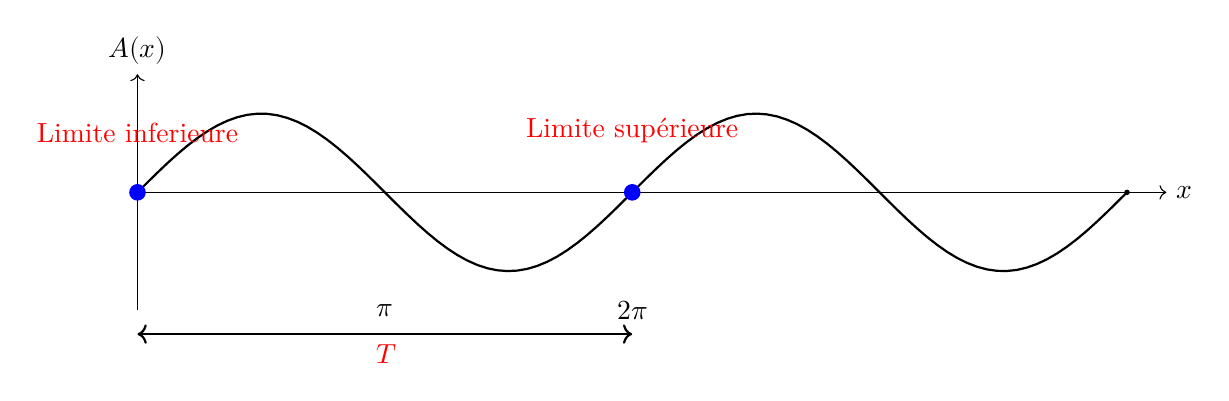
\begin{tikzpicture}[scale=1]
  % Tracé de la courbe sinusoïdale
  \draw[thick, domain=0:4*pi, samples=100] plot (\x, {sin(\x r)});

  % Axe horizontal
  \draw[->] (0,0) -- (4*pi + 0.5, 0) node[right] {$x$};

  % Axe vertical
  \draw[->] (0,-1.5) -- (0,1.5) node[above] {$A(x)$};

  % Indication de la période
  \draw[<->, thick] (0, -1.8) -- (2*pi, -1.8) node[midway, below, red] {$T$};

  % Marquage de la période
  \node at (pi, -1.5) {$\pi$};
  \node at (2*pi, -1.5) {$2\pi$};

  % Points clés pour la période
  \fill[blue] (0,0) circle (3pt);
  \node[above, red] at (0,0.5) {Limite inferieure};
  \fill[blue] (2*pi,0) circle (3pt) ; 
  \node[above, red] at (2*pi,0.5) {Limite supérieure};
  \fill (4*pi,0) circle (1pt);
\end{tikzpicture}
\caption{l'application des conditions au limites donne $A(0)=0$ et $A(2\pi)=0$}
 
\end{figure}

Par exemple, fixons nous un intervalle de définition 0, T et cherchons
les fonctions propres de B qui vérifient la condition : \(f(0)=f(T0)\)

d'oú pour \(\omega\) la suite de valeurs :

\[\omega=0,\frac{2\pi}{T}, \frac{4\pi}{T}...\frac{k2\pi}{T}...\]

Les fonctions propres de l'opérateur \[B=\frac{d^2}{dx^2}\] qui
vérifient la condition de périodicité aux limites sur l'intervalle (O,
T) sont donc de la forme :

\[e^{\frac{ik2\pi x}{T}}\] et \[e^{\frac{-ik2\pi x}{T}}\]

Nous pouvons considérer ces fonctions comme des vecteurs généralisés
complexes.

Il nous faut étendre à ces vecteurs fonctionnels complexes la définition
du produit scalaire rencontrée dans le cas des vecteurs fonctionnels
réels : il s'agira du \emph{produit hermitien}.

\subsection{3.21 Produit scalaire hermitien de deux vecteurs
fonctionnels complexes
:}\label{produit-scalaire-hermitien-de-deux-vecteurs-fonctionnels-complexes}

Soient \(f(x)\) et \(g(x)\) deux fonctions complexes d'une variable
réelle \(x\), définies sur l'intervalle O, T et \(\overline{f(x)}\) et
\(\overline{g(x)}\) leurs conjuguées.

A ces fonctions correspondent les vecteurs :

\[\left| f \right\rangle, \left| g \right\rangle\]

et

\[\left\langle f \right|, \left\langle g \right|\]

Le produit hermitien :

\[\boxed{\left\langle f|g \right\rangle=\frac{1}{T}\int_{0}^{T} \overline{f(x)} g(x)\,dx}\]

\subsection{3.22 Propriété d'orthogonalité
:}\label{propriuxe9tuxe9-dorthogonalituxe9}

Les vecteurs fonctionnels complexes \(\left|f\right\rangle\) et
\(\left| g \right\rangle\) sont dit ``orthogonaux'' si le produit
hermitique est nul. On a alors :

\[\left\langle f|g \right\rangle = \left\langle g|f \right\rangle = 0\]

Les fonctions propres de l'opérateur \[\frac{d^2}{dx^2}\] sont
orthogonales.

\emph{Il revient au même de parler de ``fonctions orthogonales'' ou de
``vecteurs orthogonaux'' puisque nous avons montré que les fonctions
envisagées sont assimilables à des vecteurs.}

\subsection{3.23 Norme :}\label{norme}

On appelle norme du vecteur fonctionnel complexe :
\(\left|f\right\rangle\) le produit hermétique de ce vecteur par
lui-même soit :

\[N \left| f \right\rangle = \left\langle f \right| \left| f \right\rangle = \frac{1}{T} \int_{0}^{T} \overline{f(x)} f(x)\,dx=\frac{1}{T} \int_{0}^{T} |f(x)|^2dx\]
Lorsque nous parlerons plus tard de la fonction d'onde représentée par
le vecteur \(\Psi\), nous dirons que la norme au carre de \(\Psi\) est :
\[\langle \Psi | \Psi \rangle=|||\Psi\rangle||^2=\sum_{i}c_i^*c_i=\sum_{i}|c_i|^2\]

\subsection{\texorpdfstring{3.24 Norme des fonctions propres de
\(\frac{d^2}{dx^2}\)
:}{3.24 Norme des fonctions propres de \textbackslash frac\{d\^{}2\}\{dx\^{}2\} :}}\label{norme-des-fonctions-propres-de-fracd2dx2}

La norme des vecteurs de la suite \(\left| f_k \right\rangle\) c'est à
dire la norme des fonctions propres \[e^{ik\frac{2\pi}{T}x}\] de
l'opérateur \[\frac{d^2}{dx^2}\] a pour valeur :

\[|\vec{f}| = \left\langle f \right| \left| f \right\rangle = \frac{1}{T} \int_{0}^{T} e^{-ik\frac{2\pi}{T}x} e^{ik\frac{2\pi}{T}x} \,dx=\frac{1}{T} \int_{0}^{T}dx=1\]
Les vecteurs de la suite \(\left| f_k \right\rangle\) ont donc pour
norme l'unité.

L'ensemble des vecteurs propres de l'opérateur \(\frac{d^2}{dx^2}\)
orthogonaux et normés à l'unité forment un système orthonormé. On
établit qu'ils peuvent être utilisés comme vecteurs de base et ainsi
servir à la décomposition de n'importe quel autre vecteur.

On exprime cette propriété en disant que la suite des vecteurs propres
est complète.

\subsection{3.25 Développement complexe de fourier
:}\label{duxe9veloppement-complexe-de-fourier}

\begin{quote}
\textbf{Rappel de traitement du signal :}
\end{quote}

\begin{quote}
Séries de fourier :
\[f(x)=\sum _{n=-\infty }^{+\infty }c_{n}(f){e}^{{i}2\pi {\tfrac {n}{T}}x}\]
Coefficients de fourrier
\[c_{n}(f)={\frac {1}{T}}\int _{T}f(t){e}^{-{i}2\pi {\tfrac {n}{T}}t}\mathrm {d} t.\]
\end{quote}

\begin{quote}
Transformée de fourier appliquée à la quantique : (Najib 2022)
\end{quote}

\begin{quote}
TF de f(x) périodique de période T :
\[g(k)=\frac{1}{\sqrt{2\pi}}\int_{-\infty}^{+infty}f(x)e^{-ikx}dx\] La
transformation inverse est donnée par :
\[f(x)= \frac{1}{\sqrt{2\pi}}\int_{-\infty}^{+infty}g(k)e^{ikx}dk\] La
valeur du paramètre \(k\) sera vu un peu plus loin dans un exercice.
\end{quote}

Sous forme algébrique, la décomposition d'un vecteur fonctionnel sur la
base des vecteurs propres de l'opérateur \[\frac{d^2}{dx^2}\] se traduit
par l'identité :

\[f(x)=\sum _{n=-\infty }^{+\infty }C_{n}{e}^{{i}2\pi {\tfrac {n}{T}}x}\]
dans laquelle nous supposerons que f(x) est une fonction réelle de la
variable réelle x définie sur l'intervalle O,T. On reconnait sous cette
forme le développement de f(x) en série complexe de fourier. Les
coefficients C\_n se calculent par la formule de fourier :

\[c_{n}(f)={\frac {1}{T}}\int _{T}f(t){e}^{-{i}2\pi {\tfrac {n}{T}}t}\mathrm {d} t.\]

\subsubsection{Théorème de Dirac :}\label{thuxe9oruxe8me-de-dirac}

Si f(x) est fonction propre de A avec la valeur propre associé a, f(x)
est également fonction propre de \(A^2\) avec la valeur propre associé
\(a^2\) carré de la précédente.

Après avoir fait le choix d'un intervalle de définition avec des
conditions aux limites, nous appellerons \emph{opérateur fonctionnel
hermétique} un opérateur qui admet un système orthogonal complet de
fonctions propres et dont les valeurs propres associées sont toutes
réelles. C'est le cas de l'opérateur \[\frac{d^2}{dx^2}\] qui est donc
un opérateur hermitique.

L'importance de opérateurs hermitiques provient de ce que tous les
opérateurs de la mécanique quantique qui représentent des grandeurs
physiques sont des opérateurs hermitiques.

L'opérateur \[\frac{d^2}{dx^2}\] est un opérateur réel car il ne
contient pas le symbole ``i'' mais la théorie s'applique plus
généralement au cas d'opérateurs complexes tels que par exemple les
opérateurs que nous rencontrerons en mécanique quantique :

\[\frac{h}{i2\pi}\frac{d}{dx}\] \[\frac{h}{i2\pi}\frac{d}{dy}\]
\[\frac{h}{i2\pi}\frac{d}{dz}\] \[-\frac{h}{i2\pi}\frac{d}{dt}\]

\subsection{3.26 Base des fonctions propres d'un opérateur fonctionnel
hermitique
:}\label{base-des-fonctions-propres-dun-opuxe9rateur-fonctionnel-hermitique}

Pour les opérateurs que nous aurons à utiliser, les n fonctions propres
forment un système \emph{complet} ce qui permet de mettre toute fonction
f(x) sous la forme d'un développement qui généralise le développement de
fourier soit :

\[f(x)=a_1f_1(x) + a_2 f_2(x) + ... + a_n f_n(x)\] Dans ce
développement, \(f(x)\) peut être une fonction réelle ou complexe, comme
les fonctions propres \(f_1(x), f_2(x)...\) elles-mêmes.
\(a_1, a_2, ... a_n\) sont des nombres complexes dans le cas général.

Ainsi sur la base des fonctions propres de l'opérateur hermitique A, le
vecteur fonctionnel \[\left| f \right\rangle\] représentatif de la
fonction \(f(x)\) peut être mis sous la forme matricielle unicolonne :

\[\left| f \right\rangle=\begin{pmatrix}
a_1 \\
a_2 \\
. \\
. \\
. \\
a_n \\
\end{pmatrix}\]

De même prenant les conjugués des deux membres du développement,

\[\overline{f(x)}=\overline{a_1}\overline{f_1(x)} + \overline{a_2}\overline{f_2(x)} + ... + \overline{a_n} \overline{f_n(x)}\]

On voit que l'on peut écrire le vecteur fonctionnel
\(\left\langle f \right|\) représentatif de la fonction conjuguée
\(\overline{f(x)}\) sous la forme uniligne :

\[\left\langle f \right|=\begin{pmatrix}
a_1 & a_2 & . & . & . a_n \\
\end{pmatrix}\]

Les fonctions propres et leurs complexes conjugués se comportent comme
des vecteurs de base.

Nous verrons plus loin lorsque nous parlerons de la fonction d'onde
\(\psi\) la définition suivante :

Si on appelle \(\psi(\vec(r))\) la fonction d'onde représentée par le
ket \(|\psi\rangle\) dans une base donnée :

\[|\psi\rangle=\sum_{i} c_i|u_i\rangle\] l'ensemble des vecteurs
\({|u_i|}\) constituant une base de l'espace des états quantiques.

\subsection{3.27 Représentation d'un opérateur fonctionnel par une
matrice
:}\label{repruxe9sentation-dun-opuxe9rateur-fonctionnel-par-une-matrice}

Considérons maintenant un opérateur fonctionnel B, hermitique ou non,
distinct de A. Toute fonction f(x) est transformée par B en une autre
fonction g(x) suivant :

\[g(x)=Bf(x)\]

Remplacons dans cette egalite fonctionnelle la fonction f(x) par son
développement, il vient :

\[g(x)=a_1Bf_1(x) + a_2Bf_2(x) + ... + a_nBf_n(x)\]

et chacune des fonctions transformées

\(Bf_1(x)\) \(Bf_2(x)\) \(...\) \(Bf_n(x)\)

est elle même développable dans le cas général su la base des fonctions
propres :

\(f_1(x)\) \(f_2(x)\) \(f_n(x)\)

suivant :

\(Bf_1(x)=B_1^1f_1(x) + B_2^1f_2(x) + ... + B_n^1f_n(x)\)
\(Bf_2(x)=B_1^2f_1(x) + B_2^2f_2(x) + ... + B_n^2f_n(x)\)

\(Bf_n(x)=B_1^nf_1(x) + B_2^nf_2(x) + ... + B_n^nf_n(x)\)

Ainsi aur la base des fonctions propres de A, l'opérateur fonctionnel B
est représentable par la matrice :

\[|B|=\begin{pmatrix}
B_1^1  & B_1^2 & ... & B_1^n \\
B_2^1  & B_2^2  & .... & B_2^n \\
.....  & .....& ....& ....\\
B_n^1 & B_n^2 & ... & B_n^n \\ 
\end{pmatrix}\]

On reconnait les relations qui ont servi à définir une transformation
matricielle. Elles font passer des composantes du vecteur \(|f\rangle\)
aux composantes du vecteur \(|g\rangle\) suivant :

\[\begin{pmatrix}
a_1'  \\
a_2'  \\
.....  \\
a_n'  \\ 
\end{pmatrix}= \begin{pmatrix}
B_1^1  & B_1^2 & ... & B_1^n \\
B_2^1  & B_2^2  & .... & B_2^n \\
.....  & .....& ....& ....\\
B_n^1 & B_n^2 & ... & B_n^n \\ 
\end{pmatrix}.\begin{pmatrix}
a_1  \\
a_2  \\
.....  \\
a_1  \\ 
\end{pmatrix}\]

Pour plus d'élégance on peut écrire les intégrales sous forme
vectorielle puisqu'elles représentent des produits hermitiques.

Par exemple on notera \(B_2^1=\left\langle f_2\right|B|f_1\rangle\)

La matrice représentative de l'opérateur B s'écrit alors :

\[|B|=\begin{pmatrix}
 \left\langle f_1 \right|B|f_1\rangle & \left\langle f_1 \right|B|f_2\rangle & ... & \left\langle f_1 \right|B|f_n\rangle \\
\left\langle f_2 \right|B|f_1\rangle  & \left\langle f_2 \right|B|f_2\rangle  & .... & \left\langle f_2 \right|B|f_n\rangle \\
.....  & .....& ....& ....\\
\left\langle f_n \right|B|f_1\rangle & \left\langle f_n \right|B|f_2\rangle & ... & \left\langle f_n \right|B|f_n\rangle \\ 
\end{pmatrix}\]

Ce sont les notations utilisées par Dirac.

\subsection{3.28 Calcul pratique des éléments de la matrice
B}\label{calcul-pratique-des-uxe9luxe9ments-de-la-matrice-b}

(Wiggins 2024) page 21

\begin{quote}
Projection operator Let \(P : V \to V\) be a linear operator on a vector
space V. Then P is said to be a projection operator if \(P^2=P\).
\end{quote}

\begin{quote}
Spectral theorem for finite dimentional self-adjoint operators : Let A :
V \to V be a self adjoint linear operator on a finite dimentionnal
complex inner product space. Then : - A has real eignevalues, and the
eignevectors of A corresponding to distincts eignevalues are orthogonal.
- the eigenvectors of A span V.
\end{quote}

\subsubsection{3.28.1 Exemple 1 : opérateur
dérivée.}\label{exemple-1-opuxe9rateur-duxe9rivuxe9e.}

Si B est l'opérateur \[\frac{d}{dx}\], et si nous adoptons pour base
orthonormée les fonctions propres de l'opérateur \[\frac{d^2}{dx^2}\]
déterminées précédemment : \[e^{in\frac{2\pi}{T}x}\]

nous trouvons :

\[B_2^1=\frac{1}{T}\int_{0}^{T}e^{-2i\frac{2\pi}{T}x} \frac{d}{dx} e^{i\frac{2\pi}{T}x},dx\]
\[=\frac{1}{T}i\frac{2\pi}{T}\int_{0}^{T}e^{-2i\frac{2\pi}{T}x} e^{i\frac{2\pi}{T}x},dx\]
\[=i\frac{2\pi}{T^2}\int_{0}^{T}e^{-i\frac{2\pi}{T}x}dx=0\] Plus
généralement on vérifierait que les éléments non diagonaux de la matrice
représentative \(\frac{d}{dx}\) sont tous nuls.

Calculons de la même façon les éléments diagonaux de la matrice.

On obtient :

\[B_n^n=\frac{1}{T}\int_{0}^{T}e^{-ni\frac{2\pi}{T}x} \frac{d}{dx} e^{ni\frac{2\pi}{T}x},dx\]

\[=\frac{in2\pi}{T^2}\int_{0}^{T}dx=\frac{in2\pi}{T}\]

Sur cette base la matrice représentative de \[\frac{d}{dx}\] est donc de
la forme:

\[B=\begin{pmatrix}
-ni\omega  & 0 & 0 & 0 & 0 & 0 & 0 & 0 & 0 & 0 \\
....  & ....  & .... & .....& ... & ... & ... & ... & ... & ... \\
0  & 0 & -3i\omega & 0 & 0 & 0 & 0 & 0 & 0 & 0 \\
0 & 0 & 0 & -2i\omega & 0 & 0 & 0 & 0 & 0 & 0 \\
0 & 0 & 0 & 0 & -i\omega  & 0 & 0 & 0 & 0 & 0 \\
  0  & 0  & 0  & 0 & 0 &  0 & 0 & 0 & 0 & 0 \\
   0    & 0  & 0 & 0 & 0 & 0 & iw & 0 & 0 & 0 \\
    0   & 0  & 0  & 0 & 0 & 0 & 0 & 2i\omega & 0 & 0 \\
     0 & 0  & 0  & 0 & 0 & 0 & 0 & 0 & 3i\omega  & 0 \\
     ..    & ..  & ..  &.. & .. &...  & ... & .... & .....& ...  \\
      ..    & ..  & ..  &.. & .. &...  & ... & .... & ..... & ni\omega \\
\end{pmatrix}\]

Les termes diagonaux de la forme ni \(\frac{2\pi}{T}\) ne sont pas réels
donc la matrice n'est pas hermitienne. Mais on obtiendrait une matrice
hermitienne en considérant l'opérateur : \[\frac{1}{i}.\frac{d}{dx}\]

Le raisonnement se généralise et permet de représenter sous forme
matricielle les opérateurs de dérivation successives
\(\frac{d^n}{dt^n}\).

Ces matrices sont toutes diagonales car elles ont le même système de
vecteurs propres. Les valeurs propres sont les termes diagonaux, ce sont
:

Pour l'opérateur \(\frac{d}{dt}\) :

\(-2i\omega_0\) \(-i\omega_0\) \(0\) \(i\omega_0\) \(2i\omega_0\)

Pour l'opérateur \(\frac{d^2}{dt}^2\)

\(-4\omega_0^2\) \(-\omega_0^2\) 0 \(-\omega_0^2\) \(-4\omega_0^2\)

Selon (Wiggins 2024) : Consider an approximately defined vector space of
complex valued differentiable functions of a real scalar variable x.
Then a liear operator on this vector space can be defind by
differentiation as follows : \((A\Phi)(x)=-i\frac{d\Phi}{dx}(x)\)

\subsubsection{\texorpdfstring{3.28.2 Exemple 2 : matrice non diagonale.
Opérateur
\(x*\)}{3.28.2 Exemple 2 : matrice non diagonale. Opérateur x*}}\label{exemple-2-matrice-non-diagonale.-opuxe9rateur-x}

Adoptons maintenant pour l opérateur B l'opérateur de multiplication x *

Le terme général \(B_p^q\) est :

\(B_p^q=\frac{1}{T}\int_{0}^{T}e^{-pi\frac{2\pi}{T}x}xe^{qi\frac{2\pi}{T}x}dx\)

avec \(p\) et \(q\) entier, et \(p\neq q\)

\section{Mesure quantique}\label{mesure-quantique}

\subsection{3.29 Représentation d'une grandeur physique par un
opérateur}\label{repruxe9sentation-dune-grandeur-physique-par-un-opuxe9rateur}

Un système physique en mouvement étant décrit par une fonction d'onde
\(\phi(x,y,z,t)\) on convient de faire correspondre des opérateurs aux
grandeurs physiques qui lui sont attachées.

Ainsi à la fonction \(g(x,y,z,p_x,p_y,p_z,E)\) on associera l'opérateur
:
\[g[x,y,z,\frac{h}{i2\pi}\frac{d}{dx},\frac{h}{i2\pi}\frac{d}{dy},\frac{h}{i2\pi}\frac{d}{dz},-\frac{h}{i2\pi}\frac{d}{dt}]\]L'opérateur
agit sur une fonction : la fonction \(\phi\) du système.

\subsection{3.30 Nouvelle notion de mesure
:}\label{nouvelle-notion-de-mesure}

Comme nous le savons, étant donné un opérateur A, il possède un spectre
de fonctions propres et de valeurs propres définies par l'égalité :
\(A\Psi=a\Psi\)

Le système étant décrit par la fonction d'onde \(\Psi\), et la grandeur
étudiée par l'opérateur A :

\begin{enumerate}
\def\labelenumi{\arabic{enumi}.}
\tightlist
\item
  Si \(\Psi\) n'est pas fonction propre de A, la grandeur est
  inobservable, aucune mesure précise n'est possible.
\item
  Si \(\Psi\) est fonction propre de A, la mesure de la grandeur, qui
  doit être un nombre, est la valeur propre \(a\) associée.
\end{enumerate}

\subsection{8.2 Mesure quantique}\label{mesure-quantique-1}

Dans certaines sciences, comme l'électronique, effectuer une mesure d'un
système influe sur ce dernier. Il est possible de dire que : « j'observe
donc je perturbe. ». En effet, lorsque l'on effectue une mesure sur un
circuit électronique, il faut prendre en compte le fait que l'appareil
de mesure est également un élément du circuit. Il peut disposer de sa
propre résistance par exemple. Ainsi, effectuer une mesure revient à
interagir avec le système. (Cluzel, Mazel, and Hill 2020) .

il y a une notion irréversibilité associée à la mesure quantique comme
pour la blockchain.

Bohr (BOHR 1928) écrit :

\begin{quote}
Des lignes spectrales qui selon la théorie classique devraient provenir
d'un même état de l'atome sont attribuées, d'après le postulat
quantique, a différents processus de transition entre lesquels l'atome a
le choix.
\end{quote}

Par exemple en théorie classique ma voix est la somme de toutes mes
fréquences alors qu'en quantique un état correspond a un niveau parmi
plusieurs possibles.

\begin{quote}
Selon (Wiggins 2024) page 67 : Measurement :
\end{quote}

\begin{itemize}
\item
  the state of a physical system is described by a normalized ket,
  \(|\Psi \rangle\), in a hilbert space \(\mathcal{H}\).
\item
  every measurable physical quantity of a physical system is described
  by a self adjoint operator A acting on the Hilbert space
  \(\mathcal{H}\). We now give a brief description of the three
  ``rules'' or postulates of measurement (..) formulated in a paper of
  Max Born published in 1926 : Zur Quantenmechanik der Stoßvorgänge
\item
  outcome of a measurement : the only possible outcome of the
  measurement of a physical observable A is an eignevalue of A,
  \(\lambda\).
\item
  Probability for a particular outcome of a measurement : suppose the
  system is in the state \(|\Psi \rangle\) and the observable A is
  measured. When the eigenvalue of A, \(\lambda\), occurs with the
  probability :
  \[prob_{\Psi}(\lambda)\equiv\langle\Psi|P_{\lambda}|\Psi\rangle=||P_{\lambda}|\Psi\rangle||^2\]
  where \(P_{\lambda}\) is the orthogonal projection onto the subspace
  spanned by the eignevectors corresponding to \(\lambda\).
\item
  State of the system after measurement : If the measurement of A on the
  system that is in the state \(|\Psi\rangle\) gives the outcome
  \lambda, when the state of the system after the measurement is given
  by :
  \[\frac{P_{\lambda}|\Psi\rangle}{\sqrt{\langle{\Psi|P_{\lambda|\Psi\rangle}}}}\]
\end{itemize}

\subsection{9.1 Historique de l'interpretation statistique
:}\label{historique-de-linterpretation-statistique}

En 1939, Fritz London et Edmond Bauer ont écrit : (London and Bauer
1939)

\begin{quote}
L'interprétation statistique de la mécanique ondulatoire peut être
considérée comme une tentative particulièrement conservatrice pour
maintenir l'image de Bohr et d'Einstein et l'encadrer en un système
théorique cohérent.
\end{quote}

Einstein avait du mal à accepter que les lois de la physique ``se jouent
aux dés''. Malgré tout, le formalisme mathématique statistique appliqué
à la physique quantique a formé un cadre acceptable. A noter que la
physique statistique ne concerne pas que la quantique mais par exemple
la thermodynamique comme présenté dans le cours de François Chevoir
(Chevoir 2013).

\subsection{9.2 Précisions concernant le symbolisme matriciel
:}\label{pruxe9cisions-concernant-le-symbolisme-matriciel}

A la fonction \(\phi\) correspond le KET : \(|\phi \rangle\) A la
fonction conjuguée \(\bar \phi\) le BRA : \(\langle\phi|\)

La décomposition de la fonction \(\phi\) sur un système orthonormal
complet de fonctions propres sera symbolise vectoriellement par :

\[|\phi\rangle=c_1|\phi_1\rangle + c_2|\phi-@\rangle + ... + c_3|\phi_n\rangle\]
Il faut relier le formalisme mathematique et les faits physiques.

Nous associerons la décomposition du suivant :
\[\langle\phi|=\bar c_1 \langle \phi_1 | + \bar c_2 \langle \phi_2 | + ... + \bar c_n \langle \phi_n |\]

En tenant compte des lois d'orthogonalité :

\[\langle \phi_i | \phi_j \rangle>=0\]

Ainsi en posant :

\[\bar c_1 c_1 = |c_1|^2\]

\[\bar c_2 c_2 = |c_2|^2\]

\[\bar c_n c_n = |c_n|^2\]

On obtiendra :

\[\langle \phi | \phi \rangle = |c_1|^2 \langle \phi | \phi \rangle + |c_2|^2 \langle \phi | \phi \rangle + ... + |c_n|^2 \langle \phi | \phi \rangle\]

\(|c_1|^2\) est la probabilité que le système saute dans l'état
\(\phi_1\), \(|c_2|^2\) est la probabilité que le système saute dans
l'état \(\phi_2\)

Si on utilise la condition de normalisation :

\[\langle \phi_i | \phi_i \rangle>=1\]

On obtient :

\[\langle \phi_i | \phi_i \rangle=|c_1|^2 + |c_2|^2 + ... + |c_n|^2\]

On a deux conceptions :

\begin{enumerate}
\def\labelenumi{\arabic{enumi}.}
\item
  présence simultanée de divers états selon des taux définis ou
\item
  passage du système de l état \(|\phi\rangle\) à l'un ou l'autre des
  états propres de A.
\end{enumerate}

Adoptons la seconde interprétation. Nous supposons qu'à l'instant de
l'observation le système soit dans l état propre \[|\phi\rangle\].

La signification physique de l'expression :
\[\langle \phi_n | A | \phi_n \rangle\] est donc simple : c'est la
mesure exacte de A lorsque le système est dans l'état \(\phi_n\)

Essayons de comprendre le sens plus général de l'expression :
\[\langle\phi|A| \phi\rangle\] (première interprétation).

\[\langle\phi|A| \phi\rangle=|c_1|^2 a_1 + |c_2|^2 a_2  + ... +  |c_n|^2 a_n\]
La signification de cette expression est celle d'une moyenne prise sur
tous les états propres possibles, chaque état étant pondéré par une
coefficient égal à sa probabilité d'existence.

Examinons un autre cas ou le système est dans un état propre
\(|\phi_{n}\rangle\) de l'opérateur A et ou on tente de mesurer une
autre grandeur représenté par un opérateur B non commutable avec A. Si
nous exigeons des mesures précises, cette tentative est vouée à l'échec.

Nous pouvons former les expressions :

\[\langle\phi_n|A|\phi_n\rangle\] \[\langle\phi_n|B|\phi_n\rangle\] La
première est la mesure exacte de A, la seconde est une valeur moyenne de
B.

Je vous renvoi vers le livre d'Augustin Blaquiere (Blaquière 1960) pour
ces développements.

Selon (Wiggins 2024) page 17 :

\begin{quote}
Let A be a linear operator on \(\mathbb{C}^2\) We consider
\(A|\Psi \rangle\) and the inner product of this vector with another
vector \(|\phi\rangle\)
\((|\phi\rangle,A|\Psi \rangle)=\langle\phi|A|\Psi\rangle\) This is
referred to the expectation value of A in the state \(|\Psi\rangle\)
\(A_{ij}=\langle e_{i}|A|e_{j}\rangle\)
\end{quote}

\subsection{9.3 Récapitulatif :}\label{ruxe9capitulatif}

La valeur moyenne de A dans l'état \(\phi\) est définie par :

\[\langle A\rangle _{\psi }=\langle \psi |A|\psi \rangle\]

Ne pas confondre \(A_{ij}=<u_{i}|A|u_{j}>\) qui donne la valeur des
éléments matriciels dans la base discrète \({|u_{i}|}\) et
\(\langle A\rangle=\langle\Psi|A|\Psi\rangle\) qui est la valeur moyenne
de l'opérateur A dans l'état \(|\Psi\rangle\).

Ainsi la valeur moyenne de l'observable position \(X\) et l'impulsion
\(P_{x}\) dans la representation \({|x\rangle}\) s'ecrivent :

\[\langle X \rangle=\langle \Psi | X | \Psi \rangle=\int_{+\infty}^{-\infty}\Psi^*(x)x\Psi(x)dx\]
\[\langle P_{x} \rangle=\langle \Psi | P_x | \Psi \rangle=-i\hbar\int_{+\infty}^{-\infty}\Psi^*(x)\frac{d\Psi(x)}{dx}dx\]

\section{5. L'onde de Louis De Broglie
:}\label{londe-de-louis-de-broglie}

\subsection{5.1 Equation des ondes ou de d'Alembert
:}\label{equation-des-ondes-ou-de-dalembert}

Le scientifique français Jean le Rond d'Alembert, qui a établi
l'équation des ondes en une dimension d'espace en 1746.
\[\frac {\partial ^{2}{\vec {\mathrm {E} }}}{{\partial x^{2}}} + \frac {\partial ^{2}\vec {\mathrm {E} }}{\partial y^{2}} + {\frac {\partial ^{2}{\vec {\mathrm {E} }}}{\partial z^{2}}}={\frac {1}{c^{2}}}{\frac {\partial ^{2}{\vec {\mathrm {E} }}}{\partial t^{2}}}\]
On remarque que le terme qui représente l'énergie est en dérivée
seconde.

\subsection{5.2 La thèse de De Broglie de 1924
:}\label{la-thuxe8se-de-de-broglie-de-1924}

Dans sa thèse de 1924, Louis de Broglie écrit : (Broglie 1924)

\begin{quote}
``L'électron est pour nous le type du morceau isolé celui que nous
croyons, peut-être à tort, le mieux connaître ; or d'après les
conceptions reçues, l'énergie de l'électron est répandue dans tout
l'espace avec une très forte condensation dans une région de très
petites dimensions dont les propriétés nous sont d'ailleurs fort mal
connues. Ce qui caractérise l'électron comme atome d'énergie, ce n'est
pas la petite place qu'il occupe dans l'espace, je répète qu'il l'occupe
tout entier, c'est le fait qu'il est insécable, non sula- divisible,
qu'il forme une unité. Ayant admis l'existence d'une fréquence liée au
morceau d'énergie, cherchons comment cette fréquence se manifeste a
l'observateur fixe dont il fut question plus haut.''
\end{quote}

On lit que Louis de Broglie admet une fréquence liée : c'est le début de
la relation onde-corpuscule.

\subsection{5.3 Concept d'onde de matière
:}\label{concept-donde-de-matiuxe8re}

L'électron étant une particule matérielle on appelle par extension onde
matérielle l'onde associée à une particule.

On représente cette onde par la fonction d'onde complexe :
\[\boxed{\Psi(\vec{r},t)=ae^{-i(wt-k\vec{r})}}\] avec :

\begin{itemize}
\tightlist
\item
  \(a\) étant l'amplitude,
\item
  \(k\) le vecteur d'onde,
\item
  \(\omega\) la pulsation,
\item
  \(\nu\) etant la fréquence.
\item
  \(\vec{p}=\hbar \vec{k}\) le vecteur impulsion
\end{itemize}

On peut ainsi trouver la forme suivante :

\[\Psi(\vec{r},t)=ae^{-i(Et-\vec{p}\vec{r})/\hbar^2}\]

Dans sa forme cette onde ressemble à une onde plane monochromatique que
l'on utilise en optique,

Voici la \emph{relation de de Broglie ou relation de la longueur d'onde
de de Broglie} :

\[\boxed{p=\frac {h}{\lambda}}\] \(\lambda\) étant la longueur d'onde de
l'onde de De Broglie.

Elle traduit la dualité onde-corpuscule en associant la longueur d'onde
\(\lambda\) d'un rayonnement à la quantité de mouvement \(p\) d'une
particule.

On trouve la forme suivante : \[\lambda=\frac{2\pi}{k}\].

Ces relations sont également valables pour les photons.

Toutefois la vitesse de phase de l'onde de De Broglie n'est pas la
vitesse de la particule mais une valeur approchée. Ainsi De Broglie
envisage qu'une particule n'est pas représentée par une onde sinusoïdale
pure mais par une superposition de plusieurs ondes sinusoïdales appelées
paquet d'ondes.

La relation \(\lambda=\frac{h}{p}\) ne joue pas le rôle de postulat de
base. Toutefois elle a permis d'arriver à la conclusion qu'il faut voir
un lien entre la position de la particule et celle de l'amplitude du
paquet d'ondes.

Une onde plane n'étant pas de carré sommable, ce n est pas véritablement
une fonction d' onde. Toutefois une onde plane peut être une première
approximation d' une fonction d' onde. La fonction d'onde est une
superposition linéaire d'ondes planes.

\section{6. Principe d'incertitude d'Heisenberg
:}\label{principe-dincertitude-dheisenberg}

\subsection{6.1 Expérience courante du principe d'incertitude
:}\label{expuxe9rience-courante-du-principe-dincertitude}

\emph{Quand un objet va vite, sa trajectoire est plus difficile à
décrire (je perds sa position) comme s'il fallait choisir entre vitesse
et position.} \emph{Par exemple, pour suivre la trajectoire d'un oiseau,
je suis obligé de le suivre du regard pour identifier sa trajectoire :
je compense l'incertitude par la multiplicité des mesures.}

La vitesse de l'oiseau n'apparaît comme n'étant rien d'autre que le
résultat d'un changement de position : il semble y avoir un lien de
causalité entre vitesse et position dans le sens ou tout changement de
position de l'oiseau se fait à une certaine vitesse.

A Nice sur la promenade des anglais il y a des petites chaises bleues
sur le front de mer ou les passants s'assoient. Un jour dans le vieux
Nice j'ai vu un magasin de souvenirs qui vendaient les mêmes chaises
bleues mais en miniature. Si j'en achete une et que le vendeur l'emballe
dans une petite boite, quelle est l'incertitude sur la position de la
chaise dans la boite ?

\begin{center}
\includegraphics[width=1.04167in,height=\textheight,keepaspectratio]{chaise.png}
\end{center}

Ainsi Niels Bohr (BOHR 1928) dit, en citant Heisenberg :

\begin{quote}
``On peut même dire, remarque-t-il à ce sujet, que les phénomènes
ordinaires (macroscopiques) sont en quelque sorte engendrés par des
observations répétées.''
\end{quote}

Cette approche accorde de importance à l'expérience. Pour Heisenberg si
l'expérience montre une impossibilité a déterminer avec précision une
position alors il faut l'admettre comme fondement et faire avec.

Concernant une position, par exemple, je regarde la feuille d'un arbre
qui fait 5 cm de long. Elle est localisable devant moi. Imaginons que la
feuille ait une longueur infiniment grande. Dans ce cas quelle est
l'incertitude sur la position de cette feuille géante \(\Delta x\), est
ce \(0\) ou \(+\infty\)

Conclusion : ce paragraphe introductif pour but de vous faire vous poser
des questions à partir constations simples de la vie courante.

\subsection{6.2 Principe d'incertitude des radioelectriciens
:}\label{principe-dincertitude-des-radioelectriciens}

En principe le terme de principe d'incertitude des radioelectriciens
n'est pas l'objet d'un usage. Il est toutefois cité par Augustin
Blaquiere (Blaquière 1960). Je choisis de le mettre en valeur dans ce
cours car il a un intérêt pédagogique : en effet il fait le pont entre
une notion classique et une notion quantique. Dans le cas classique nous
sommes tous familiarisés avec le fait par exemple que le son de la voix
peut être représentée par son spectre.

Le principe d'incertitude est une propriété \emph{mathématique des
séries de fourier}. Il n'est pas spécifique à la physique quantique.
Ainsi on le retrouve en électronique lorsqu'on on associe à un signal
temporel un spectre en fréquence. Toutefois il existe des différences
entre les deux :

En électronique on raisonne systématiquement sur une amplitude (tension
ou intensité) en fonction du temps, en physique quantique on parle le
plus souvent d'une amplitude fonction de x.

Pour l'électronicien le principe d'incertitude prendra la forme
\(\Delta t \times \Delta f \approx 1\)

Lorsque le signal est une impulsion brève dans le temps, la gamme de
fréquence est très étendue mais les fréquences sont très serrées.
Lorsque \(\Delta t\) tend vers 0 (impulsion breve) le spectre devient
continu.

Avec le principe d'incertitude de radioelectriciens on ne prend pas en
compte la condition de quantification présente dans la relation :
\(E=h\mu\)

Il est intéressant de remarquer que dans un cas classique (électronique
ou acoustique) si il est possible d'avoir une bande de fréquence très
étirée (voir infinie) ce n'est pas en général la bande de fréquence
``utile''. Par exemple :

\begin{enumerate}
\def\labelenumi{\arabic{enumi}.}
\item
  En électronique on a l'habitude de fabriquer des filtres passe haut,
  passe bas ou passe bande afin d'éliminer les fréquences excentrées qui
  constituent du bruit.
\item
  En acoustique, le timbre d'une voix humaine est un mélange de
  différentes fréquences. Personne n'a une voix ``monocorde''. Toutefois
  ici encore le message utile à la compréhension d'une voix humaine est
  regroupé sur une bande de fréquence limitée. On peut remarquer que en
  cas de bruit de fond, dans une salle très bruyante par exemple, à
  condition de se concentrer il est possible d'isoler la conversation
  qui nous intéresse comme si le cerveau avait une capacité de filtrage
  sélective. De même l'oreille réussit à isoler des sons isolés. Autre
  exemple : dans une salle de restaurant bruyante, si une cuillerée
  tombe par terre, on isole très bien cet ``évènement'' du bruit de fond
  constitué des autres sons.
\end{enumerate}

\subsection{6.3 Transposition au domaine électromagnétique
:}\label{transposition-au-domaine-uxe9lectromagnuxe9tique}

Toutefois on peut se demander si un principe équivalent au principe
d'incertitude des radioelectriciens existe dans le cas d'ondes
électromagnétiques c'est à dire d'ondes lumineuses.

Nous savons qu'en quantique il y a une condition de quantification
(\(E=h\nu\)). nous savons depuis l'expérience du corps noir que cette
condition s'applique aux ondes lumineuses. Mais que se passe t il si on
applique pas la condition de quantification et qu'on en reste a \(\nu\)
et pas à \(E\).

Bohr était un bon pédagogue et des 1928 il a pu communiquer une synthèse
assez aboutie. Rappelez vous de la photo de la page 5 qui correspond au
congre Solvay de 1927. Celui-ci a permis les discussions que l'on
appelle quelquefois par abus de langage le ``consensus de Copenhague''.

Ainsi Bohr (BOHR 1928) décrit cette forme première du principe
d'incertitude avant quantification en prenant l'exemple d'une onde plane
élémentaire ayant la forme :
\[A\cos 2 \pi(\nu t -\sigma x -\sigma y -\sigma z + \delta)\] ou \(A\)
et \(\delta\) sont des constantes désignant l'amplitude et la phase ;
\(\mu\) est la fréquence ; \(\sigma x\), \(\sigma y\) et \(\sigma z\)
sont les nombres d'onde dans les directions des axes.

Alors selon Bohr, stricto sensu la représentation d'un champ d'ondes
limite exige une multiplicité d'ondes élémentaires correspondant à
toutes les valeurs possibles de \(\nu\) e de \(\sigma\). Cependant
\emph{dans les cas les plus favorables} les valeurs moyennes des
différentes grandeurs (\ldots) seront données par la relation :
\[\Delta t \Delta \nu = \Delta x \Delta \sigma x =  \Delta y \Delta \sigma y =  \Delta z \Delta \sigma z =1\]

\subsection{6.4 La publication de 1925 d'Heisenberg : vers un nouveau
formalisme
:}\label{la-publication-de-1925-dheisenberg-vers-un-nouveau-formalisme}

Revenons un peu en arriere. En 1924 alors qu'il n'est age que de 24 ans
et qu'il n'a pas encore sa thèse, Heisenberg écrit : (Heisenberg 1925)

\begin{quote}
``Dans cette situation, il paraît judicieux d'abandonner tout espoir
d'observer des grandeurs jusqu'ici inobservables, comme la position et
la période d'un électron, et d'admettre que l'accord partiel entre les
règles quantiques et l'expérience est plus ou moins fortuit. Au lieu de
cela, il semble plus raisonnable de tenter d'établir une mécanique de la
théorie quantique analogue a la mécanique classique, mais dans laquelle
seules apparaissent des relations entre des grandeurs observables.''
\end{quote}

On voit dans l'extrait ci-dessus que l'objectif d'Heisenberg est de ne
baser l'interprétation que sur des résultats observables. Ainsi il
s'agit de ``renoncer'' à une interprétation au delà de ce que la mesure
peut nous donner.

Ceci est la première publication d'Heisenberg. Elle pose un formalisme
base sur des tableaux. Heisenberg parlera de matrices un peu plus tard.
Il posera le principe d'incertitude qui porte son nom en 1927.

Ainsi Andre Coret (Coret 2001) écrit : ``En s'appuyant sur l'expérience
c'est a dire sur la nécessite de considérer l émission lumineuse comme
issue d'un changement d'état de l electron et non de son mouvement,
Heisenberg se permet une opération qu'il qualifie lui-même d'arbitraire
(willkur).''

\subsection{6.5 Apport du formalisme hamiltonien
:}\label{apport-du-formalisme-hamiltonien}

Sir William Rowan Hamilton était un physicien irlandais du 19 eme
siècle.

Fritz London et Edmond Bauer écrivent : (London and Bauer 1939)

\begin{quote}
L'évolution du système dans le temps est réglée en mécanique classique
par une ``fonction hamiltonienne'' H(p,q) caractéristique du système en
question. Cette fonction de coordonnées q1,q2,\ldots,qf et des
impulsions p1,p2,pf (..) permet d'écrire les fonctions hamiltoniennes du
mouvement. C'est cette même fonction H(q,p) qui en mécanique quantique
aussi donne la loi d'évolution du représentant \phi de l'état du système
: on forme l'opérateur \(H(q,\frac{h}{2\pi i\frac{\delta}{\delta q}})\)
en remplaçant p dans l'hamiltonien par l'opérateur de différentiation :
\(\frac{h}{2\pi i\frac{\delta}{\delta q}}\)
\end{quote}

On voit qu'en formalisme hamiltonien le paramètre t n'est plus visible.
Le temps passe, t est sous entendu mais ce n'est pas lui qui apparaît
dans la formule mais q la position et p la quantité de mouvement. On va
par exemple décrire le diagramme de phase d'un oscillateur harmonique
classique en fonction de p et de q. (et non pas par exemple de q et de
t). \emph{On prend l'habitude ``en douceur'' de lier les variables de
position et de quantité de mouvement.} Ce formalisme hamiltonien est
lui-même une branche de ce que l'on appelle la physique analytique.

\subsection{6.6 Approche intuitive de la non commutation des fonctions
:}\label{approche-intuitive-de-la-non-commutation-des-fonctions}

Il s'agit ici, à titre préparatoire au principe d'incertitude lui-même,
d'aborder les choses sous un angle différent. Il existe bien un lien la
notion de commutation et le principe d'incertitude. Lorsque l'on parle
de commutation on pense d,abord a des matrices. Par exemple si A et B
sont des matrices, si le produit : \(AB-BA=0\) on dit que les matrices
commutent. On sait aussi que la plupart du temps le produit de 2
matrices n'est pas commutatif.

Toutefois Augustin Blaquiere (Blaquière and Jean 1960) présente une
approche basée sur les fonctions :

Nous allons voir que \(x \times\) et \(\frac{d}{dx}\) ne sont pas
commutables lorsqu'on les applique à une fonction f(x).

On a en effet : \[\frac{d}{dx}[xf(x)]=x\frac{d}{dx}f(x) + f(x)\]

en effet : \((uv)'=u'v+uv'\)

d'ou

\[\frac{d}{dx}[xf(x)] -x\frac{d}{dx}f(x)=f(x)\]

que l'on traduit symboliquement par :

\[(\frac{d}{dx}x -x\frac{d}{dx})f(x)=f(x)\]

ou sous une forme plus condensée, par :

\[\frac{d}{dx}x -x\frac{d}{dx}=1\]

\subsection{6.7 Cas limites du principe d'incertitude
:}\label{cas-limites-du-principe-dincertitude}

J'appelle cas limites les situations ou soit l'incertitude sur la
position est tres elevee, soit l'incertitude sur la vitesse est tres
elevee, mais pas les deux en meme temps ou aucun des deux.

(Wichmann, Lallemand, and Ostrowsky 1974)

Ces cas sont ceux pour lesquels :

\(\Delta x \Delta p \approx 1\)

Au contraite nous verrons que la forme la plus generale du principe
d'inceertitude sera celle d'une inegalité

\begin{center}
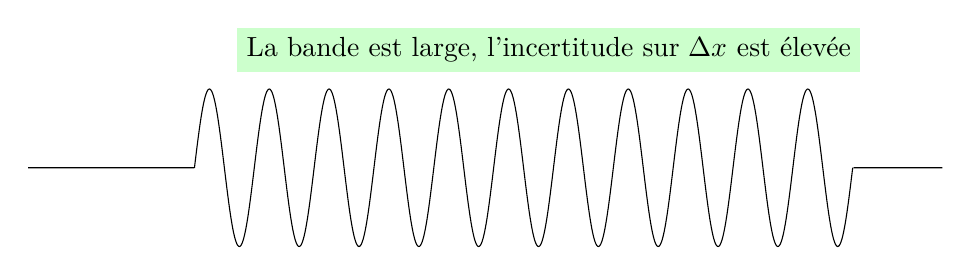
\begin{tikzpicture}[x=3.8cm/360]
  \pgfplothandlerlineto
\pgfplotfunction{\x}{-200,-199,...,0}{\pgfpointxy{\x}{0}}
\pgfplotfunction{\x}{0,1,...,792}{\pgfpointxy{\x}{sin(5*\x)}}
 
\pgfplotfunction{\x}{793,794,...,900}{\pgfpointxy{\x}{0}}
  \pgfusepath{stroke}
\draw (4.5cm,1.5cm)  node [fill=green!20] {La bande est large, l'incertitude sur $\Delta x$ est élevée};
\end{tikzpicture}
\end{center}

Par exemple dans le cours de Berkeley (Wichmann, Lallemand, and
Ostrowsky 1974) il est donné en exemple les cas ou une des 2 formes
d'incertitude est franche dans le cas d'un electron en ``orbite'' autour
d'un noyau :

\begin{enumerate}
\def\labelenumi{\arabic{enumi}.}
\item
  Si l'électron est confine dans une très petite région autour du noyau,
  l'incertitude sur sa position est faible. l'incertitude sur sa
  quantité de mouvement doit être grande, ce qui signifie que son
  énergie cinétique doit être grande.
\item
  Si vous voulons que l'énergie cinétique soit très petite nous devons
  accorde assez de place a l'électron : l'incertitude sur sa position
  doit être grande, sa distance moyenne au noyau doit alors être grande.
\end{enumerate}

\begin{center}
 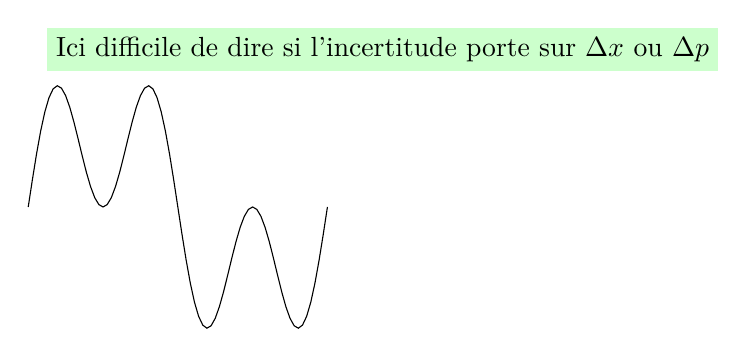
\begin{tikzpicture}[x=3.8cm/360]
  \pgfplothandlerlineto
  \pgfplotfunction{\x}{0,5,...,360}{\pgfpointxy{\x}{sin(\x)+sin(3*\x)}}
  \pgfusepath{stroke}
  \draw (4.5cm,2cm)  node [fill=green!20] {Ici difficile de dire si l'incertitude porte sur $\Delta x$ ou $\Delta p$};
\end{tikzpicture}
\end{center}

\subsection{6.8 Premier principe d'incertitude d'Heisenberg
:}\label{premier-principe-dincertitude-dheisenberg}

La relation suivante limite les precisions avec lesquelles on peut
mesurer la position et l'impulsion :

\[\boxed{\Delta x \times \Delta p \geq \frac{\hbar}{2\pi}}\] C'est le
premier principe d'incertitude d'Heisenberg.

Avec :

\(\Delta x\) indétermination sur la position

\(\Delta p\) indétermination sur la quantité de mouvement de la
particule

\(\hbar\) est le symbole utilisé en physique pour représenter la
constante de Planck réduite. Elle est une version simplifiée de la
constante de Planck, notée généralement \(h\), divisée par \(2\pi\).

Attention à la portée de ce principe : il ne s'agit pas d'une contrainte
expérimentale liée par exemple aux instruments du laboratoire mais de
plus que cela. Nous pouvons le considérer comme un fondement
théorique.\emph{C'est independant des instruments utilisés.}

\subsection{6.10 Principe d'incertitude temps energie
:}\label{principe-dincertitude-temps-energie}

On l'appelle aussi second principe d'incertitude d'Heisenberg.

Ce n'est pas la traduction du premier principe en d'autres termes mais
quelaue chose de different.

On a parlé du principe d'incertitude des radioelectriciens :
\[\Delta t \times \Delta f \approx 1\]

On peut l'utiliser par exemple en acoustique dans l'analyse
fréquentielle d'un son.

Appliquons lui maintenant la condition de quantification :

\(E=h\mu\)

La relation d'incertitude des radioelectriciens devient :

\[\Delta t \times \Delta \frac{E}{h} \approx 1\]

\[\Delta t \times \Delta E \approx h\]

Ce qui donne lorsqu'on le généralise :

\[\boxed{\Delta E \times \Delta t \geq \frac{\hbar}{2}}\]

Il s'agit du second principe d'incertitude d'Heisenberg ou inégalité
d'Heisenberg énergie-temps.

Avec :

\(\Delta E\) l'incertitude sur énergie du système. \(\Delta t\)
l'intervalle de temps pendant lequel le système reste dans un état
énergétique.

Par exemple plus la durée de vie d'un état quantique est courte, plus
l'incertitude sur son énergie est grande.

On voit ici que c'est la condition de quantification qui fait que ce
second principe existe. Cela traduit le fait que quand la fequence est
elevee l'energie associee est importante. Ce fait qui fut decouvert par
planck n'est pas intuitif du tout.

\subsection{6.12 Base en représentation par t
:}\label{base-en-repruxe9sentation-par-t}

La problématique de départ est plus compliquée ici. Une derivee
représente un intervalle entre 2 positions. Pour être dans une
représentation en position on s'intéresse a un simple point dans
l'espace. Toutefois dans notre démarche nous allons commencer par poser
les choses en t et non pas en x comme si le point auquel on s'interesse
mais pas un point dans l'espace mais dans le temps. Nous nous
intéressons donc a un intervalle très court sur la ligne du temps et
nous l'assimilons a une impulsion de Dirac.

Physiquement parlant, une impulsion de Dirac peut se comparer en terme
temporel a une timbale qui émet un son fort mais très bref. On va ainsi
filtrer le signal sur un intervalle temporel très petit.

\begin{figure}
\centering
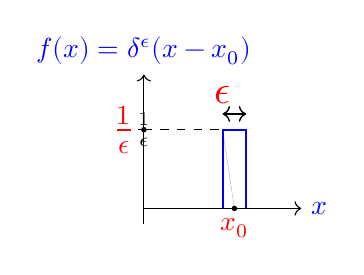
\begin{tikzpicture}
  % Définir la largeur epsilon
 % \def\epsilon{0.2}
  
  % Tracer l'axe horizontal
  \draw[->] (0,0) -- (2,0) node[right, blue] {$x$};
  \draw[->] (0,-0.2) -- (0,1.7) node[above, blue] {$f(x)=\delta^{\epsilon}(x-x_{0})$};
  
  % Tracer la fonction créneau
  \draw[thick, blue] 
    (1,0) -- (1,1) -- (1.3,1) -- (1.3,0);
  
  % Optionnel : ajouter des points ou des annotations
  \fill (0,1) circle (1pt);
  \fill (1.15,0) circle (1pt) node[below, red] {$x_{0}$} -- (1,1);
%  \fill (0.5+\epsilon,1) circle (1pt);
%  \fill (1,0) circle (1pt);

\draw[dashed] (0,1) node[left, red] {\Large $\frac{1}{\epsilon}$} -- (1,1) ;
  
  % Ajouter des labels
 \node at (0, 1) {$\frac{1}{\epsilon}$};

 \draw[<->,line width=0.5pt] (1,1.2) node[above, red] {\Large $\epsilon$} -- (1.3,1.2) ;

\end{tikzpicture}
\end{figure}

\begin{quote}
\textbf{Rappel} (Najib 2022) La distribution de dirac appelée par abus
de language fonction \(\delta\) de dirac est informellement considérée
comme une fonction \(\delta(x-x_{0})\) qui n'a de valeur qu'au voisinage
de \(x_{0}\) et qui prend une valeur infinie en ce point et la valeur 0
partout ailleurs, et dont l'intégrale sur tout l'espace est égale à 1.
Considérons \(\delta^{\epsilon}(x-x_{0})=1\), alors
\(\int_{-\infty}^{+\infty}\delta^{\epsilon}(x-x_{0})=1\). La fonction de
dirac est definie par :
\(\delta(x-x_{0})=\lim_{x \to 0}\delta^{\epsilon}(x-x_{0})\)
\end{quote}

Nous raisonnons en t. Une impulsion peut être un signal très bref en
termes temporels. Toutefois en termes spatiaux cela peut se représenter
par une distance très courte. Ici encore la fonction impulsion
\(\delta x\) s'applique

\subsection{6.13 Utilité de la fonction porte
:}\label{utilituxe9-de-la-fonction-porte}

\(\delta x\) est une vue théorique car sa largeur est nulle. En pratique
nous allons utiliser la fonction échelon mais sur une distance très
courte : c'est la fonction porte.

\begin{figure}
\centering
  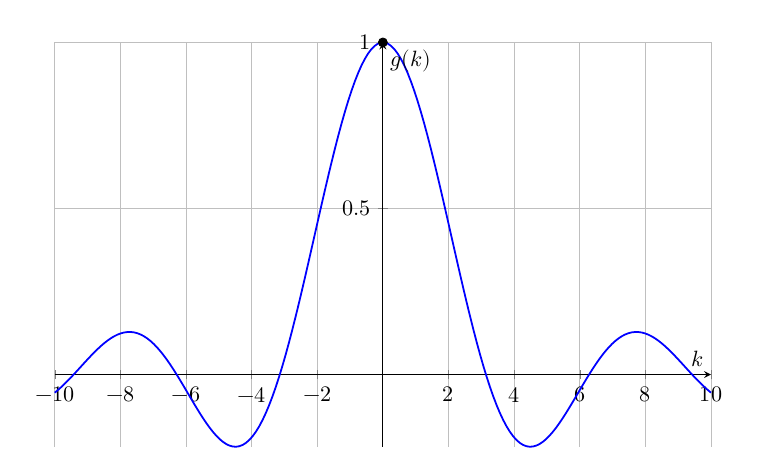
\begin{tikzpicture}[scale=0.8]
  \begin{axis}[
    domain=-10:10,
    samples=200,
    axis lines=middle,
    xlabel=$k$,
    ylabel=$g(k)$,
    xtick={-10,-8,...,10},
    ytick={-0.5,0,0.5,1},
    height=8cm,
    width=12cm,
    grid=both,
    clip=false
  ]
    \addplot [blue, thick] {sin(deg(x))/x};
    \addplot [mark=*, only marks] coordinates {(0,1)};
  \end{axis}
\end{tikzpicture}
\caption{La fonction sinus cardinal qui est la TF de la fonction porte ici prise en exemple sur l'intervel [-10,10]}
\end{figure}

Attention :

\begin{enumerate}
\def\labelenumi{\arabic{enumi}.}
\item
  La solution de l'équation de Schrödinger est une gaussienne dans le
  cas d'une particule libre. Dans le cas d'une particule confinée dans
  un puits de potentiel on se ramène à une onde stationnaire.
\item
  Contrairement au cas de la lumière, pour le particule le milieu est
  dit dispersif, ce qui signifie que la gaussienne (c'est a dire la
  densité de probabilité) va s'étaler (s'aplatir) sur une surface de
  plus en plus grande au cours du temps.
\end{enumerate}

\subsection{6.15 Conséquence : concept de paquet d'onde
:}\label{consuxe9quence-concept-de-paquet-donde}

Nous devons parler ici du cas de la particule libre qui n'est pas
confinée dans un espace comme c'est le cas dans un puits de potentiel.

La longueur d'onde de de Broglie implique du fait du principe
d'incertitude que \(\Delta x=+\infty\). Dans ce cas, on ne sait pas où
chercher ce qui rend la mesure impossible.

On dit que la particule n'est pas normalisable.

Physiquement, on est pas dans le cas de figure d'un électron qui gravite
autour d'un atome mais dans celui d'une particule qui évolue librement
dans un espace très grand. Du fait qu'elle est soumise a peu
d'interactions d'origine électromagnétique on peut imaginer que sa
vitesse est faible. Dans un cas idéal, déterminer sa position de façon
très précise revient à comparer \(\delta x\) une impulsion de Dirac.

On va remplacer l'impulsion de Dirac par une fonction porte, ce qui va
agir comme un filtre sur les fréquences. La bande infinie des fréquences
va se retrouvée ramenée à une bande constituée d'ondes de fréquences
très proches.

Par addition ces fréquences vont former une gaussienne, le paquet
d'ondes.

Par principe de superposition, toutes ondes étant la somme d'ondes
solutions de l'équation de Schrödinger est elle-même solution de
l'équation de Schrödinger.

\subsection{6.16 Vitesse de phase et vitesse de groupe
:}\label{vitesse-de-phase-et-vitesse-de-groupe}

Nous continuons à parler d'une particule libre qui n'est pas soumise a
un potentiel.

On s'attend à ce que la vitesse de la particule soit celle de l'onde de
De Broglie, c'est à dire l'onde individuelle. On peut en effet associer
une vitesse \emph{de phase} à l'onde de De Broglie. Toutefois ce n'est
pas la vitesse de la particule mais une valeur approchée. C'est la
\emph{vitesse de groupe} qui constitue la vitesse de la particule.

Plus précisément :

Vitesse de phase : \[v_{phi}=\frac{w}{k}\]

Vitesse de groupe : \[v_{g}=\frac{dw}{dk|k=k_{0}}\]

\section{7. Équation de Schrödinger
:}\label{uxe9quation-de-schruxf6dinger}

\subsection{7.1 Rappel de physique des ondes
:}\label{rappel-de-physique-des-ondes}

Il s'agit simplement de faire quelques rappels terminologiques pour
éviter toutes confusions dans les termes.

\emph{Onde progressive :} une onde progressive ``progresse', par exemple
le son se propage dans l'air.

\emph{Onde stationnaire :} C'est une onde qui apparaît immobile.
Idéalement elle est la conséquences de deux ondes progressives qui
arrivent en sens opposées et interfèrent. ``Naturellement'' il faut des
conditions très précises pour s'en approcher. On peut aussi penser a la
corde d'une guitare classique qui va vibrer sur elle-même.

\emph{Onde plane :} il s'agit d'un concept plus que un onde que l'on
rencontre reelement. Toutefois c'est une modélisation suffisamment
approchée dans certains milieux comme les milieux homogènes. Il s'agit
bien d'une sinusoïde mais qui dépend d'une seule variable spatiale.

\emph{Équation d'onde :} Posée la première fois par Jean Le Rond
d'Alembert en 1747 elle s'applique en toutes les ondes en physique
classique. En physique quantique elle sera remplacée par équation de
Schrödinger.

Voici la formule de l'équation d'onde en une dimension :

\[\boxed{\frac{\partial^2 u}{\partial t^2} - c^2 \frac{\partial^2 u}{\partial x^2} = 0}\]

\subsection{7.2 Exemple tiré des télécommunications
:}\label{exemple-tiruxe9-des-tuxe9luxe9communications}

Voici l'exemple d'un circuit RLC (filtre passe bande).

Les paramètres L, C et R sont appelés des impédances.

\begin{center}
\begin{circuitikz}
    \draw (0,0) to [short] ++(0,1) node [right] {$-$}
    to [open, v^>=$E(t)$, o-o] ++(0,1) node [right] {$+$}
    to [short] ++(0,1)
    to [R=$R$, i>^=$I$, resistors/zigs=6] ++(4,0)
    to [curved capacitor, l_=$C$, capacitors/thickness=8] ++(0,-3)
    to [cute inductor, l_=$L$, mirror] ++(-4,0);
\end{circuitikz}
\end{center}

La tension et l'intensite sont des grandeurs electriques que l'on peut
representer par des sinusoides. Le comportement du circuit est decrit
par une equation differentielle :

\[
 \left\{
    \begin{array}{ll}
        L\frac{di(t)}{dt} =-Ri(t) -V_{c}(t) -e(t) \\
        i(t)=C\frac{dv_{c}(t)}{dt}
    \end{array}
\right.
\]

Notez qu'il s'agit d'une représentation fonctionnelle et on est tenté de
remplacer les variables par des matrices. Ce n'est toutefois pas
possible de façon directe.

Pour utiliser des matrices, l'équation doit être modifiée de la façon
suivante :(Dixneuf and Bellouvet 2007)
\[\frac{dX(t)}{dt}=\begin{bmatrix}
-R/L & -1/L \\
1/C & 0 
\end{bmatrix}X(t)+\begin{bmatrix}
-1/L  \\
0 
\end{bmatrix}U(t)\]\\
Dans ce cas X(t) est un vecteur d'état qui représente par exemple le
courant. C'est une ``vision moderne'' ou on introduit la notion d'état
en électronique.

En physique quantique on aussi besoin d'une équation différentielle pour
décrire évolution de l'état d'un corpuscule.

C'est l'équation de Schrödinger.

\emph{Elle est régi par des opérateurs qui sont l'équivalent des
impédances.}

La solution de l'équation de Schrödinger est la fonction d'onde.

\subsection{7.3 Extrait de la publication de Schrödinger de
1926}\label{extrait-de-la-publication-de-schruxf6dinger-de-1926}

Erwin Schrödinger écrit : (Schrödinger 1926)

\begin{quote}
Je ne saurais passer sous silence que je dois l'impulsion première qui a
fait éclore ce travail pour la plus grande part a la remarquable thèse
de Louis de Broglie. (\ldots) la principale différence entre ses
résultats et les nôtres consiste en ce que monsieur de Broglie imagine
de sondes progressives tandis que si on interprète nos formules au
moyens d'une hypothèse ondulatoire on est conduit a des vibrations
d'ondes stationnaires.
\end{quote}

Cet extrait exprime la différence entre l'onde de De Broglie et la
fonction d'onde solution de l'équation de Schrödinger.

\subsection{7.4 Equation de Schrödinger dépendante du temps
:}\label{equation-de-schruxf6dinger-duxe9pendante-du-temps}

\subsubsection{7.4.1 Principe de conservation de l'énergie
:}\label{principe-de-conservation-de-luxe9nergie}

Exprimons que pour une particule en mouvement dans un champ de force l'
énergie totale est la somme de l' énergie cinétique et de l' énergie
potentielle. Nous supposons le système isolé.

Soit en adoptant l'approximation non relativiste si la particule est
animée d'une assez faible vitesse (devant la vitesse de la lumière) :
\[E=\frac{p^2}{2m} + V(x,y,z)\] \(E\) est l'énergie totale de la
particule

\(V(x,y,z)\) son énergie potentielle qui ne dépend que des coordonnées
de position.

Ainsi :

\[p_x^2 + p_y^2 + p_z^2 -2m(E-V)=0\]

\subsubsection{7.4.2 Principe de correspondance
:}\label{principe-de-correspondance}

Poser une équation même si elle est juste nous conserve dans le cas de
la mécanique classique.

Toutefois nous avons vu qu'en quantique il n'existe pas une expression
d'un paramètre physique mais plusieurs qui dépendent de la base
utilisée. C'est la raison pour laquelle l'équation de Schrödinger
apparaît contre intuitive quand on la voit pour la première fois.

Voici la correspondance entre grandeurs classiques et grandeurs
quantiques :

\begin{longtable}[]{@{}lc@{}}
\toprule\noalign{}
Classique & Quantique \\
\midrule\noalign{}
\endhead
\bottomrule\noalign{}
\endlastfoot
\(E\) & \(i\hbar\frac{d}{dt}\) \\
\(p\) & \(-i\hbar\nabla\) \\
\(x\) & \(x\) \\
\end{longtable}

Ceci correspond à une représentation en position. Si nous utilisons une
représentation en impulsion, la base est différente et les valeurs
associées aux grandeurs seront différentes.

A titre d'illustration dans le cas classique p correspond a une grandeur
physique et dans le cas quantique à un opérateur.

Un opérateur agit sur une fonction : la fonction d'onde \(\Psi\)
solution de l'équation de Schrödinger.

\subsubsection{7.4.3 Expression de l'équation de Schrodinger dépendante
du temps
:}\label{expression-de-luxe9quation-de-schrodinger-duxe9pendante-du-temps}

Remplaçons les termes par les opérateurs qui leurs sont associés.

Nous obtenons :
\[\frac{h^2}{8\pi^2m}[\frac{d^2\Psi}{dx^2}+\frac{d^2\Psi}{dy^2}+\frac{d^2\Psi}{dz^2}]-\frac{h}{i2\pi}\frac{d\Psi}{dt} -V(x,y,z)\Psi=0\]
\emph{C'est l'équation de Schrödinger.}

On pose habituellement :

\[\nabla^2 f = \frac{\partial^2 f}{\partial x^2} + \frac{\partial^2 f}{\partial y^2} + \frac{\partial^2 f}{\partial z^2}\]

Et en remplacant \(\frac{h}{2\pi}\) par \(\hbar\)

on obtient :

\(\boxed{-\frac{\hbar}{2m}\nabla^2\Psi(r,t)+V(r,t)\Psi(r,t)=i\hbar\frac{\partial}{\partial t}\Psi(r,t)}\)

Attention à l' expression de l' énergie cinétique : il ne s'agit pas
d'une dérivée en t mais en x. Ce n' est donc pas la représentation
classique de la vitesse mais l'expression de p exprimée dans une base en
x. Ainsi l' équation de Schrödinger est une représentation en x. Si on
voulait une représentation en p, il s'agit d'une autre formulation de
l'équation.

Il faut remarquer que l'énergie totale du système est bien elle une
fonction du temps mais il s'agit d'une dérivée première et pas d'une
dérivée seconde. En cela elle se différencie de l'équation d'onde.

\subsubsection{7.4.4 Formulation moderne de l'équation de Schrödinger
dépendante du temps
:}\label{formulation-moderne-de-luxe9quation-de-schruxf6dinger-duxe9pendante-du-temps}

Nous utilisons le formalisme posé par Dirac dont nous avons longuement
parlé dans ce cours avec l'utilisation des BRA et des KETS :

\[\boxed{{i}\hbar {{\textrm {d}} \over {\textrm {d}}t}|\Psi (t)\rangle ={\frac {{\hat {\vec {P}}}^{2}}{2m}}|\Psi (t)\rangle +V{\Bigl (}{\hat {\vec {R}}},t{\Bigr )}|\Psi (t)\rangle}\]

\subsubsection{7.4.5 Fonction d'onde solution de l'équation de
Schrodinger dépendante du temps
:}\label{fonction-donde-solution-de-luxe9quation-de-schrodinger-duxe9pendante-du-temps}

Nous savons que l'onde de De Broglie est une solution de l'équation de
Schrodinger et représente une onde plane. La fonction d'onde représente
une somme d'ondes de De Broglie et il est normal qu'elle ait la forme
d'une onde plane.

\[\boxed{\psi(\vec{r},t)=ae^{-i\frac{(Et-\vec{p}\vec{r}}{\hbar}}}\]

\subsection{7.5 Equation de Schrodinger indépendante du temps
:}\label{equation-de-schrodinger-induxe9pendante-du-temps}

On se ramene ici dans le cas ou le potentiel est independant du temps :
\(V(r,t)=V(r)\)

Le terme etat stationnaire provient de l'interpretation de la norme au
carre de la fonction d'onde en tant que densite d eprobabilite (la norme
au carre est independante du temps).

On utilise une methode de separation de variables :

\(\Psi(r,t)=\phi(r)f(t)\)

L'équation de Schrödinger indépendante du temps s'écrit sous la forme
suivante :

\[ \boxed{ \left[ -\dfrac{\hbar^2}{2m} \nabla^2 + U(r) \right] \phi(r) = E \phi(r) } \]

où :

\begin{itemize}
\tightlist
\item
  \(\hbar\) est la constante de Planck réduite,
\item
  \(m\) est la masse de la particule,
\item
  \(\nabla^2\) est l'opérateur Laplacien (en coordonnées cartésiennes :
  \(\frac{\partial^2}{\partial x^2} + \frac{\partial^2}{\partial y^2} + \frac{\partial^2}{\partial z^2})\),
\item
  \(U(r)\) est l'énergie potentielle en fonction de la position \(r\),
\item
  \(\phi(r)\) est la fonction d'onde indépendante du temps,
\item
  \(E\) est l'énergie totale de la particule (valeur propre associée à
  la fonction d'onde).
\end{itemize}

Dans ce cas, \(\phi(\vec{r})\) est la composante position de
\(\Psi(\vec{r},t)\)

\[\Psi(\vec{r},t)=\phi(\vec{r}).\underbrace{e^\frac{-iEt}{\hbar}}_{\text{Composante dependante du temps}}\]\\
Ceci ne constitue pas une solution générale mais particulière.

Voici la solution générale :

\[\Psi(r,t)=\Sigma c_{k}(0)e^\frac{-iEt}{\hbar}\phi_{k}(r)\]

\subsection{Application : etats propres de l'opérateur d'énergie pour le
puit de potentiel
infini:}\label{application-etats-propres-de-lopuxe9rateur-duxe9nergie-pour-le-puit-de-potentiel-infini}

Selon (Wiggins 2024) un etat staionnaire peut decrire une particule
libre a partir du moment ou elle n'est soumise a aucun potentiel. Ainsi.
page 32 : We consider the general case where the potential energy is
independant of time, i e : V(r,t)=V(r). The schrodinger equation can be
solved using the method of separation of variables. We assume a solution
on the form : \(\phi(r,t)=\Phi(r)f(t)\) The time independant state
equation : \(\frac{-\hbar^2}{2m}\nabla^2\Phi(r) + V(r)\Phi(r)=E\Phi(r)\)
A solution is given by :
\(\Psi(r,t)=\Phi(r)f(t)=\Phi(r)f(0)e^{\frac{-i}{h}Et}\) (2.8) f(0) is a
constant : an arbitrary constant can be dealt with through normalization
and the choice of initial conditions. The origin of the term stationnary
state comes from the interpretation of the magnitude squared of the wave
function as a probability density (the magnitude squared is independant
of time). (2.8) is not the general solution. It is merely a paerticular
solution : General solution :
\(\Psi(r,t)=\Sigma c_{k}(0) e^{\frac{-iE_{k}}{\hbar}t}\Psi_k(r)\)

Niels Bohr décrit (BOHR 1928) ainsi l'état stationnaire :

\begin{quote}
La réalité des états stationnaires : le concept d'état stationnaire
résulte, on l'a déjà dit, d'une application caractéristique du postulat
quantique au système considéré. Par sa nature, ce concept exige que l'on
fasse complètement abstraction d'une description temporelle (\ldots)
Strictement parlant, le concept d'état stationnaire implique l'exclusion
de toute interaction avec des ``individus'' qui n'appartienne pas au
système.
\end{quote}

On peut interpréter ce que dit Bohr comme la constatation de la
fragilité de l'état stationnaire par rapport aux perturbations
extérieurs.

L'énergie d'un système est mesurable s'il se trouve dans un état propre
de cet opérateur. Ces états privilégiés sont appelés états
stationnaires.

Les fonctions propres de l'opérateur énergie sont définies par
l'équation :

\[-\frac{h}{2i\pi}\frac{d\phi}{dt}=E\phi\]

E étant la valeur propre associée à la fonction propre
\[\phi{x,y,z,t}\].

Les fonctions \phi{x,y,z,t} qui vérifient l'équation sont de la forme :
\[\phi=u(x,y,z)e^{-i2\pi\frac{E}{h}t}\] u étant une fonction qui ne
dépend \textbf{que des variables d'espace}

La fonction u apparaît comme une fonction propre de l'opérateur :
\[H=-\frac{h^2}{8\pi^2m}\nabla^2 + V\] avec la valeur propre associée E.
On appelle H l'opérateur Hamiltonien.

On trouve la forme symbolique : \[H\phi(x)=E\phi(x)\]

qui représente l'équation de Schrödinger indépendante du temps. On peut
l'interpréter comme le fait que les valeurs propres H sont les valeurs
de E pour lesquelles l'équation admet une solution physiquement
acceptable. Une condition d'acceptabilité physique est que la fonction
d'onde soit de carré sommable. Dans le cas d'un puits de potentiel
infiniment profond cette condition conduit à la condition que la
fonction d'onde s'annule en dehors du puits.

Certains opérateurs privilégiés commutent avec le Hamiltonien. Par
exemple si NB-BH=0 la grandeur B est exactement mesurable en même temps
que l'énergie, quelle que soit l'état stationnaire, c'est a dire quelque
soit l' énergie du système. Les grandeurs physiques qui jouissent de
cette propriété sont appelées constantes du mouvement.

L'équation d'onde a dans des conditions convenables des solutions
décrivant les ondes stationnaires. Les solutions en ondes stationnaires
sont caractérisées par une dépendance temporelle de la forme
\[exp(-i\omega t)\] ou toutes les fréquences possibles forment un
ensemble discret \(\omega1\), \(\omega2\), \(\omega3\). L'énergie du n
eme état stationnaire étant donne par \(E_n=\hbar\omega_n\).

Étudions le comportement d'une particule mobile dans une direction x'x
soumise à aucune force. Le potentiel V est alors nul mais nous
supposerons que le domaine d'évolution de la particule est limité par
deux positions extrêmes P et Q qu'elle ne peut franchir. Le segment PQ a
pour longueur L. Ces conditions aux limites peuvent être traduites en
admettant que le potentiel devient infini aux points P et Q. La loi des
potentiels affecte donc la forme d'un puits rectangulaire à une
dimension aux parois impénétrables. Elles se traduisent par la nullité
de la fonction d'onde aux points P et Q.

Le hamiltonien prend la forme :
\[H=-\frac{h^2}{8\pi^2m}\frac{d^2}{dx}^2\] (V=0)

On appelle ceci l'équation de Schrödinger indépendante du temps qui
correspond à un état stationnaire. On peut le voir comme une équation
aux valeurs propres.

On trouve aussi la formulation suivante, exactement identique :

\[-{\frac{\hbar^2}{2m}\frac{d^2}{dx}^2\phi(x)}=[E-V(x)\phi{x}]\]

Ses états propres sont aussi ceux de l opérateur \[\frac{d}{dx}\]

dans le cas d'un état stationnaire la solution de l'équation de de
Schrödinger prend une forme particulière avec une composante en t et une
composante en x :

\[\Phi(x,t)=\phi(x)exp(\frac{-itE}{\hbar})\] avec
\(\hbar = \frac{h}{2\pi}\).

Les exponentielles complexes sont \[e^{in\frac{\pi}{L}x}\]

Il y a deux conditions aux limites.

1.Pour \(x=0\) alors \(\phi=0\) Le cas \(x=0\) impose comme solution
acceptable \[\phi(x)=Csin(xk)\].

\emph{En effet pour x=0 la forme la composante en cosinus ne s'annule
pas. Par contre} \(\sin(0)=0\)

2.Pour \(x=a\) alors \(\phi=0\)

\emph{On se positionne dans le cas classique de la corde vibrante.
Attention la comparaison entre classique et quantique possède ses
limites mais nous l'utilisons ici.}

pour x=L on obtient : \(\sin n\pi=1\)

Les valeurs propres de l'opérateur \[\frac{d}{dx}\] sont donc de la
forme : \[in\frac{\pi}{L}\]

et celles de l'opérateur H, compte tenu du facteur
\[-\frac{h^2}{8\pi^2m}\] sont :

\[-\frac{h^2}{8\pi^2m}{(in\frac{\pi}{L})}^2\]

Forme matricielle du hamiltonien :

\[H=\frac{h^2}{8mL^2}=\begin{pmatrix}
+\infty  & 0 & 0 & 0 & 0 & 0 & 0 & 0 & 0 & 0 \\
....  & ....  & .... & .....& ... & ... & ... & ... & ... & ... \\
0  & 0 & ... & 0 & 0 & 0 & 0 & 0 & 0 & 0 \\
0 & 0 & 0 & 4 & 0 & 0 & 0 & 0 & 0 & 0 \\
0 & 0 & 0 & 0 & 1  & 0 & 0 & 0 & 0 & 0 \\
  0  & 0  & 0  & 0 & 0 &  0 & 0 & 0 & 0 & 0 \\
   0    & 0  & 0 & 0 & 0 & 0 & 1 & 0 & 0 & 0 \\
    0   & 0  & 0  & 0 & 0 & 0 & 0 & 4 & 0 & 0 \\
     0 & 0  & 0  & 0 & 0 & 0 & 0 & 0 & ...  & 0 \\
     ..    & ..  & ..  &.. & .. & ... & ... & .... & .....&....  \\
      ..    & ..  & ..  &.. & .. & ... & ... & .... & ..... & +\infty \\
\end{pmatrix}\]

\emph{Pour les états stationnaires la densité de probabilité est
indépendante du temps. Pour les états non stationnaires elle présente
une dépendance temporelle oscillante.} Cf cours de Berkeley. (Wichmann,
Lallemand, and Ostrowsky 1974)

\section{10. Intrication quantique :}\label{intrication-quantique}

Selon (Degiovanni et al. 2020) page 168 : la notion de système
\emph{composé} suppose que l'on peut bien séparer le système complet en
deux sous systèmes sur lesquels on peut en principe faire des mesures
sans que les appareils puissent mutuellement s'influencer.

Lorsque Alain Aspect effectua ses premières expériences sur les paires
de photons intriqués à l'université d'Orsay il veilla à ce que les
mesures effectuées sur une photo ne puissent pas influencer celles
effectuées sur l'autre.

selon (Wiggins 2024) p146

\begin{quote}
Tensor product : Let \(\mathcal{H}_{A}\) and \(\mathcal{H}_{B}\) denote
finite dimensional complex linear vector spaces. each equipped with an
inner product. (i.e.~finite dimensional Hilbert Spaces). The tensor
product of \(\mathcal{H}_{A}\) and \(\mathcal{H}_{B}\) denoted
\(\mathcal{H}_{A} \otimes \mathcal{H}_{B}\) is a finite dimensional
complex linear vector space equipped with an inner product.
\end{quote}

We turn to the important issue of a basis for the tensor product space.

\begin{quote}
Orthonormal basis for the tensor product space : Let
\({|a_{i}>}, i=1,...,N_{A}\) be an orthonormal basis in
\(\mathcal{H}_{A}\) and let \({|b_{i}>}, i=1,...,N_{B}\) be an
orthonormal basis in \(\mathcal{H}_{B}\). then
\(|a_{i}\rangle \otimes |b_{j}\rangle, i=1,...,N_{A}, j=1,...,N_{B}\) is
an orthonormal basis in \(\mathcal{H}_{A} \otimes \mathcal{H}_{B}\).
Note that it follows immediately from this result that the dimension of
\(\mathcal{H}_{A} \otimes \mathcal{H}_{B}\) is \(N_{A}N_{B}\)
\end{quote}

\begin{quote}
Product state : any state
\(|\phi\rangle \in \mathcal{H}_{A} \otimes \mathcal{H}_{B}\) that can be
written on the form
\(|\phi\rangle=|\phi_{A}\rangle \otimes |\phi_{B}\rangle\) for some
\(|\phi_{A} \rangle \in \mathcal{H}_{A}\),
\(|\phi_{B} \rangle \in \mathcal{H}_{B}\) is said to be a product state
\end{quote}

\begin{quote}
Entangled state : any state
\(|\phi\rangle \in \mathcal{H}_{A} \otimes \mathcal{H}_{B}\) that cannot
be written on the form
\(|\phi\rangle=|\phi_{A}\rangle \otimes |\phi_{B}\rangle\) for some
\(|\phi_{A} \rangle \in \mathcal{H}_{A}\),
\(|\phi_{B} \rangle \in \mathcal{H}_{B}\) is said to be a entangled
state
\end{quote}

(Wiggins 2024) page 148 :

\begin{quote}
Linear operator and tensor product spaces : - Suppose A :
\(\mathcal{H}_{A} \to \mathcal{H}_{A}\) and B :
\(\mathcal{H}_{B} \to \mathcal{H}_{B}\) are linear operator. We
construct a linear operator on
\(\mathcal{H}_{A} \otimes \mathcal{H}_{B}\) using A and B. - Suppose the
linear operators \(A\) has eigenvalues \(\lambda i\) and eigenvectors
\(|a_{i} \rangle\) and suppose the linear operator B has eignevalues
\(\mu_{i}\) and eigenvectors \(|b_{i} \rangle\). Then the linear
operator \(A \otimes B\) has eignevalues \(\lambda_{i}\mu_{j}\) and
eigenvectors \(|a_{i}\rangle|b_{j}\rangle\).
\end{quote}

Un état quelconque \(|\Phi\rangle\) peut être décompose sur une base de
\(\mathcal{H}\) = \(\mathcal{H}_{A} \otimes \mathcal{H}_{B}\) comme :

\[|\Psi\rangle=\Large{\sum}_{i,j\in I_{A} \times I_{B}}^{} a_{ij} |\phi^{A}_{i}\rangle \otimes |\phi^{B}_{j}\rangle \]

ou les amplitudes a\_\{ij\} sont des nombres complexes.

Dans le cas général où plusieurs amplitudes sont non nulles l'état est
dit intriqué.

Ainsi selon Selon (Degiovanni et al. 2020) on a la figure suivante :

\usetikzlibrary {arrows.meta}
\begin{figure}
\centering
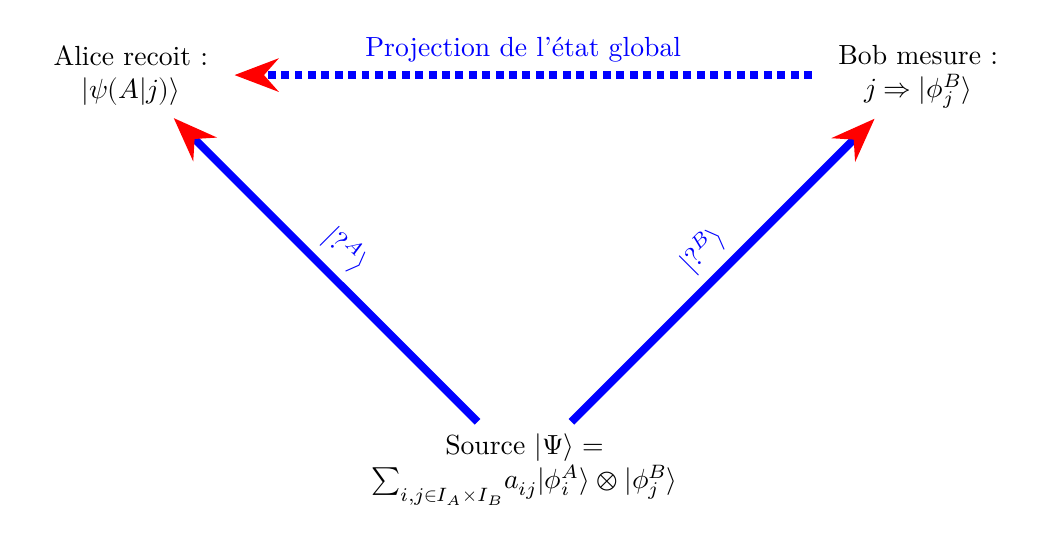
\begin{tikzpicture}
 
 \node (A) at (0,0) {\begin{tabular}{c} Source $|\Psi\rangle=$ \\ $\Large{\sum}_{i,j\in I_{A} \times I_{B}}^{} a_{ij} |\phi^{A}_{i}\rangle \otimes |\phi^{B}_{j}\rangle $ \end{tabular}};
 \node (B) at (-5,5) {\begin{tabular}{c} Alice recoit : \\ $ |\psi(A|j)\rangle$ \end{tabular}};
 \node (C) at (5,5) {\begin{tabular}{c} Bob mesure : \\ $ j \Rightarrow |\phi_{j}^{B}\rangle$ \end{tabular}};
    \draw[-{Stealth[red]},line width=1mm,blue] (A) -- (C) node[midway,sloped,above] {$|?^B\rangle$};
     \draw[-{Stealth[red]},line width=1mm,blue] (A) -- (B) node[midway,sloped,above] {$|?^A\rangle$};
      \draw[-{Stealth[red]}, dotted,line width=1mm,blue] (C) -- (B) node[midway,sloped,above] {Projection de l'état global};
\end{tikzpicture}
\caption{Une source émet un état intriqué de deux systèmes dont l'un est envoyé à Alice et l'autre a Bob. Si on considère les expériences dans lesquelles bob effectue une mesure et qu'il trouve le résultat correspondant à l'état $|\phi_{j}^B\rangle$ alors le système d'Alice est dans l'état relatif $|\psi(A|j)\rangle$.}
\end{figure}

(Wiggins 2024) page 153 : The Einstein-Podolsky-Rosen paradox

\begin{quote}
Suppose that we have a source that creates two quantum particules of
spin \(\frac{1}{2}\) One is sent to Alice and one is sent to Bob
\end{quote}

(Wiggins 2024) page 156 :

\begin{quote}
In summary, the postulate of measurement in quantum mechanics says that
if Alice measures a quantity when the state collapses to the state
corresponding to the Eigenstate of the outcome of Alice's measurement.
Therefore if Bob measure the same quantity he will obtain exactly the
same value as Alice. The result of this experience seems contrary to
common experience in two ways : - locality - reality
\end{quote}

\section{11. Informatique et information quantique
:}\label{informatique-et-information-quantique}

\subsection{11.1 Introduction :}\label{introduction}

Entre les fondements théoriques datant des années 1920-1930 abondamment
développés dans ce cours, et la période actuelle a on l'impression que
les choses ont peu avancées. En réalité, il a fallu du temps pour
réaliser les vérifications expérimentales des prédictions théoriques.
Ainsi le mécanisme de l'intrication a été vérifié seulement avec la
thèse d'Alain Aspect soutenue le 1er février 1983 au centre d'Orsay de
l'université Paris-Sud. (Aspect 1983) C'est ce décalage entre les
prédictions théoriques et les vérifications expérimentales qui
expliquent que les investissements industriels mettent beaucoup de temps
à se faire. On entend quelquefois le terme ``d'hiver quantique'' pour
qualifier cette période qui est située entre les deux révolutions
quantiques, la première étant celle qui a permis le développement de
l'électronique, et la seconde celle qui concerne l'ordinateur quantique.
En annonçant en 2019 avoir atteint la suprématie quantique, Google a
attiré l'attention du grand public. Ce terme de suprématie signifie
simplement que l'ordinateur quantique a dépassé l'ordinateur classique
en termes de performances.

En informatique classique on a longtemps parié sur la loi de Moore pour
prédire l'amélioration des capacités classiques des processeurs. Ce sont
les limites atteintes aujourd'hui qui renforcent le besoin pour la
quantique.

\subsection{11.3 Qbit - porte logique :}\label{qbit---porte-logique}

Une autre approche qui ressemble à celle de l'électronique consiste à
créer des portes logiques quantiques qui serviront de briques de base.
Par exemple en électronique le transistor est un composant qui est un
assemblage de portes logiques élémentaires. Une porte logique possède
une fonction logique.

Un qbit est une unité d'information dont l'état peut être une
superposition des états de base \(|0\rangle\) et \(|1\rangle\),
représentant simultanément 0 et 1, jusqu'à ce qu'une mesure l'effondre
vers un de ces deux états.

Mathématiquement un qbit est représenté par un vecteur colonne de
dimension 2, et une porte par une matrice \(2 \times 2\) (ou plus)

Du fait du principe de superposition, un qbit peut être dans une
infinité d'états combinaison linéaire tels que
\(\alpha |0\rangle +\beta |1\rangle\) avec
\(\left|\alpha \right|^{2}+\left|\beta \right|^{2}=1\)

Un exemple courant de porte est la fonction NOT (inversion logique)
représentable par la matrice :

\[
\begin{pmatrix}
0 & 1 \\
1 & 0 
\end{pmatrix}\]

Veuillez noter que contrairement au bit, le qubit n'a pas de valeur mais
un état. (Cluzel, Mazel, and Hill 2020). De même on pouvait voir une
porte logique comme une fonction qui calcule et retourne un résultat et
on peut voir une porte quantique comme une procédure qui effectue un
traitement et modifie ses entrées.

\subsection{11.4 Le réseau pour la quantique
:}\label{le-ruxe9seau-pour-la-quantique}

La question du consensus est un angle de vue spécifique pour aborder la
question.

A l'horizon 5 ans il faudra adapter les infrastructures actuelles pour
permettre l'émergence de l'internet quantique : à quoi ressemblera le
réseau d'interconnexion des QPUs (distributed quantum computing)?

Dans ce cas, le domaine des réseaux informatiques n'est pas une
application de la quantique mais une infrastructure réseau adaptée aux
ordinateurs quantiques constitue un besoin.

Prenons la question en sens inverse dans le paragraphe suivant.

\subsection{11.5 La quantique pour la securité réseau : le consensus
quantique
?}\label{la-quantique-pour-la-securituxe9-ruxe9seau-le-consensus-quantique}

Comme le souligne Stéphane Bortzmeyer (Bortzmeyer) dans son article de
blog le protocole TCP est la pierre angulaire du réseau internet depuis
30 ans. Le couple TCP/IP est toutefois sensible de base au
man-in-the-middle : il est possible par exemple avec une sonde réseau
d'interférer avec une trame de donnée, que ce soit dans le sens IP ou
bien TCP.

Il est tentant de remplacer la validation par TCP par une validation
décentralisée : dans le cas ou l'un des validateurs est corrompu cela
est composé par l'honnêteté des autres. Il faut toutefois avoir
confiance dans le consensus obtenu par les validateurs. \emph{Le
problème du consensus est né}.

La notion d'\emph{algorithme de consensus} quantique existe. Il s'agit
toutefois d'un thème de recherche à l'intersection de la blockchain (et
plus largement des systèmes distribués) et de la quantique. En quantique
il s'agit d'une autre façon de désigner le mécanisme de l'intrication.
Toutefois la finalité est celle d'obtenir un consensus.

Citons comme techniques d'intrication :

\begin{itemize}
\tightlist
\item
  Intrication spatiale
\item
  Intrication temporelle
\end{itemize}

Toutefois en matière de blockchain il existe deux grandes tendance de
gouvernance :

\begin{enumerate}
\def\labelenumi{\arabic{enumi}.}
\tightlist
\item
  On-chain
\item
  Off-chain
\end{enumerate}

Par on chain je veux dire : qui est situé dans le code informatique.

Dans le premier cas (off-chain) les parties prenantes vont se mettre
d'accord sur quelque chose qui sera dans un second temps intégré dans le
code par exemple sous forme d'une règle dans un smart contract.

Dans le second cas (on-chain) un consensus peut se faire sans
intervention humaine. Toutefois on peut imaginer qu'ensuite des
méchanismes de contrôle off-chain interviendront. L'algorithme de
consensus quantique etant base sur les lois de la physique (puis traduit
sous forme de code informatique) est on chain.

La dynamique on-chain / off-chain est avant tout celle d'une interaction
entre ces deux facettes de la gouvernance.

\begin{longtable}[]{@{}lc@{}}
\toprule\noalign{}
Type de consensus & Caractéristique \\
\midrule\noalign{}
\endhead
\bottomrule\noalign{}
\endlastfoot
Agrement byzantin & deterministe \\
Nakamoto consensus & probabiliste \\
Algorithme de consensus quantique & probabiliste \\
\end{longtable}

La problématique du consensus est fondamentale en matière de réseau car
elle rejoint celle de la validation en environnement décentralisé :
comment mettre d'accord des entités indépendantes.

Lorsque deux particules sont intriquées, l'information va pouvoir être
communiquée de façon instantanée entre les deux. Les deux particules
sont donc d'accord. Quelle est l'utilité de ce consensus en matière de
réseau ? Où se trouve l'intervention humaine dans ce cas ? Ce ne sont
que quelques pistes.

Le seminaire poincare (Seminar et al. 2021) met en valeur (Gheorghiu,
Kapourniotis, and Kashefi 2019) pour qui la question est :

\begin{quote}
if a quatum experiment solves a problem which is proven to be
intractable for classical computers, how caon one verify the outcome of
the experiment ?
\end{quote}

il y a plusieurs oistes possibles et les protocoles bases sur
l'intrication en est une. a ce sujet l'experience du consensus pour la
blockchain peut servir d'inspiration.

\subsection{11.6 Exercice 7 : porte quantique
:}\label{exercice-7-porte-quantique}

\emph{Source : Carpentier, Renaud, and Benoı̂t Depret. 2022.La Physique
En Applications: 140 Problèmes Corrigés Contemporains PC-MP-PMI-PSI-PT
(Carpentier and Depret 2022)}

On considère une particule se déplaçant selon les Oz croissants.
L'environnement de la particule entraîne un confinement spatial de
celle-ci de sorte qu'il existe dans le plan z=0 deux états quantiques
différents de la particule : l'état ``0'' décrit la fonction d'onde de
dépendance spatiale normalisée \(\phi_{0}(x)\) et l'etat ``1'' décrit
par la fonction d'onde de dépendance spatiale normalisée
\(\phi_{1}(x)\). On suppose aue ces deux etats sont orthogonaux c'est a
dire que : \(\int_{-\infty}^{+\infty} \phi_{0}(x) \phi_{1}(x)^* dx\) ou
l'astérisque désigne le complexe conjugué. En plus des deux états ``0''
et ``1'' qui forment un bit ``classique'' la mécanique quantique prévoit
par linéarité de l'équation de Schrodinger l'existence d'une infinité
d'états quantiques de la particule dans le plan z=0 formés par la
superposition des états ``0'' et ``1'' c'est à dire décrits par une
fonction d'onde de la forme :
\(\phi_{\alpha}(x)=\alpha\phi{0}(x) + \beta\phi_{1}(x)\) ou \(\alpha\)
et \(\beta\) sont des nombres complexes. Il est possible de choisir
\(\beta\) réel positif compris entre 0 et 1. L'etat ``\(\alpha\)''
représenté par \(\phi_{\alpha}(x)\) est appelé un ``qubit''.

\textbf{1.Qu'appelle-t-on une fonction d'onde normalisée ? Quelle est la
signification physique de la normalisation ?}

La normalisation de la fonction d'onde \(\phi(x)\) signifie que :
\[\int_{-\infty}^{+\infty} |\phi(x)|^2\ \mathrm{d}x=1\]

Solution : Or la quantite \(|\phi(x)|^2\) represente la densite de
probabilite de presence le long de l'axe Ox. La normalisation de la
fonction d'onde ets liee au fait que lorsque l'on mesure la position de
la particule, celle ci doit se trouver a un et un seul endroit.

\textbf{2. Montrer que la normalisation de l'état} \(\alpha\)'' fixe la
valeur de \(\beta\) que l'on déterminera en fonction de \(\alpha\).

Solution : La normalisarion de l'etat ``\(\alpha\)'' s'ecrit :
\[\int_{-\infty}^{+\infty} |\phi(x)|^2\ \mathrm{d}x = \int_{-\infty}^{+\infty} |\alpha\phi_{0}(x)+\beta\phi_{1}(x)|^2 dx=1)\]

\emph{Methode de résolution de l'intégrale :}

L'intégrale à résoudre est :
\[\int_{-\infty}^{+\infty} |\alpha \phi_{0}(x) + \beta \phi_{1}(x)|^2 dx\]

où \(\phi_{0}(x)\) et \(\phi_{1}(x)\) sont probablement des fonctions
orthogonales, souvent des fonctions propres dans un contexte quantique
ou mathématique, et \(\alpha, \beta\) sont des coefficients complexes ou
réels.

\emph{Développement de l'intégrale :}

En utilisant la propriété que
\[|A + B|^2 = |A|^2 + |B|^2 + 2 \Re(A \overline{B})\], l'intégrale
devient :
\[\int_{-\infty}^{+\infty} |\alpha \phi_{0}(x)|^2 dx + \int_{-\infty}^{+\infty} |\beta \phi_{1}(x)|^2 dx + 2 \Re \left( \alpha \overline{\beta} \int_{-\infty}^{+\infty} \phi_{0}(x) \overline{\phi_1(x)} dx \right)\]

\emph{Utilisation de l'orthogonalité :}

Si \(\phi0\) et \(\phi1\) sont orthogonales, alors :
\(\int_{-\infty}^{+\infty} \phi0(x) \overline{\phi_1(x)} dx = 0\)

De plus, si elles sont normalisées :
\[\int_{-\infty}^{+\infty} |\phi_{0}(x)|^2 dx = 1\]

et

\[\int_{-\infty}^{+\infty} |\phi_{1}(x)|^2 dx = 1\]

\emph{Résultat final :} Ainsi, l'intégrale se simplifie en :
\(|\alpha|^2 \times 1 + |\beta|^2 \times 1 + 0 = |\alpha|^2 + |\beta|^2\)

\emph{Conclusion :} L'intégrale est :
\[ \boxed{ \int_{-\infty}^{+\infty} |\alpha \phi_{0}(x) + \beta \phi_{1}(x)|^2 dx = |\alpha|^2 + |\beta|^2 } \]

Ce résultat est valable sous l'hypothèse que \(\phi0\) et \(\phi1\) sont
orthogonales et normalisées.

\emph{Rappel :} Propriété liée à l'identité de l'expansion du carré
d'une somme complexe La propriété
\(|a + b|^2 = |a|^2 + |b|^2 + 2 \Re(a \overline{b})\) exprime une
identité fondamentale en analyse complexe et en géométrie vectorielle.

Explication :

\(a\) et \(b\) sont des nombres complexes. \(|a|\) désigne la norme (ou
module) de \(a\), c'est-à-dire la distance de \(a\) à l'origine dans le
plan complexe. \(\overline{b}\) est le conjugué de \(b\). \(\Re(z)\)
représente la partie réelle du nombre complexe \(z\). Signification :

Cette identité montre comment le carré de la norme de la somme de deux
nombres complexes peut être décomposé en la somme des carrés de leurs
normes respectives, plus deux fois la partie réelle du produit
\(a \overline{b}\). Elle est une version complexe de la formule du carré
d'une somme en algèbre, adaptée à l'espace complexe.

Propriété associée :

Elle reflète la propriété d'expansion du carré d'une somme, qui en
géométrie vectorielle correspond à la formule du parallélogramme, et en
analyse complexe, elle permet d'établir des relations entre modules et
produits scalaires.

En résumé :

Cette formule est une propriété fondamentale de l'algèbre complexe et de
la géométrie dans le plan, souvent utilisée pour calculer la norme d'une
somme complexe ou pour analyser la relation entre deux vecteurs dans un
espace vectoriel complexe.

\emph{Propriété d'expansion du carré d'une somme} La propriété
d'expansion du carré d'une somme est une identité remarquable en algèbre
qui permet de développer rapidement l'expression ((a + b)\^{}2) en une
somme de termes plus simples.

Formule : \[(a + b)^2 = a^2 + 2ab + b^2 \]

\emph{Explication :}

Le carré de la somme d deux termes (a) et (b) est égal à : Le carré du
premier terme ((a\^{}2)), Plus deux fois le produit des deux termes
((2ab)), Plus le carré du second terme ((b\^{}2)). Propriété clé : Cette
expansion montre que le carré d'une somme n'est pas simplement la somme
des carrés, mais qu'il inclut également un terme croisé (2ab) qui
représente l'interaction entre (a) et (b).

\emph{Utilité :} Elle permet de développer rapidement des expressions
algébriques, de factoriser des trinômes ou de simplifier des calculs en
évitant de faire une multiplication complète.

\textbf{3. Le système passe à travers un système appelé opérateur
logique qui a la propriété de modifier sa fonction d'onde. La dépendance
spatiale de celle-ci s'écrit alors dans le plan de sortie} \(z=L\).

\(\phi(s.0)(x)=\epsilon_{00}\phi_{0}(x) + \epsilon_{10}\phi_{1}(x)\)
\(\phi(s.1)(x)=\epsilon_{01}\phi_{0}(x) + \epsilon_{11}\phi_{1}(x)\)

Les coefficients \(\epsilon_{ij}\) sont des nombres complexes dans le
cas general.

On appelle opeateur logique NON l'operateur lineaire qui transforme
l'etat 0 et etat 1 et reciproquement. Cet operateur existe en logiaue
quantique mais aussi en logiaue classique.

Determiner les valeurs des coefficients
\(\epsilon _{00},\epsilon _{01},\epsilon _{10},\epsilon _{11}\) de
l'operateur NON en supposant que l'operateur logique n'induit aucun
dephasage sur les fonctions d'ondes. En deduire la representation
matricielle de NON dans la base des etats \(("0","1")\) sous forme d'une
matrice \(2 \times 2\)

\emph{Solution :}

Par definition l'operateur NON n'induisant aucun dephsage \$
\phi*\{s,0\}(x)=*\phi{1}(x)\$ et \(\phi_{s,1}(x)=\phi_{0}(x)\) d'ou
\(\boxed{\epsilon_{00}=0, \epsilon_{01}=1, \epsilon_{10}=1, \epsilon_{11}=0}\)

Dans la base \(("0","1")\) on peut donc ecrire : \[NON=\begin{pmatrix}
0 & 1 \\
1 & 0 
\end{pmatrix}\]

\section{12. L'écosystème de la quantique
:}\label{luxe9cosystuxe8me-de-la-quantique}

\subsection{12.1 Les acteurs en présence
:}\label{les-acteurs-en-pruxe9sence}

Le 10 juin 2025, Station F a accueilli la 4ᵉ édition de la conférence
France Quantum (\textbf{FranceQuantum2025?}) Voici les priorités
technologiques presentee lors du salon :

\begin{enumerate}
\def\labelenumi{\arabic{enumi}.}
\item
  Intégration des processeurs quantiques dans les super ordinateurs
  exemple : Pasqal a délivré un processeur de 100 qbits au CEA.
\item
  Développer des ordinateurs quantiques tolérants aux fautes :
\end{enumerate}

\begin{itemize}
\item
  Leadé par le CEA et l'Inria à Grenoble.
\item
  Engagement sur 15 ans du ministère de la défense avec 5 starts up :
  Alice \& Bob, C12, Pasqal, Quandela, et Quobly
\end{itemize}

\begin{enumerate}
\def\labelenumi{\arabic{enumi}.}
\setcounter{enumi}{2}
\item
  Quantum sensor
\item
  Post quantum cryptographie
\item
  Quantum communication (secure quantum communication networks)
\end{enumerate}

\begin{figure}[H]

{\centering \includegraphics[width=4.16667in,height=\textheight,keepaspectratio]{ESRF.jpg}

}

\caption{L'European Synchrotron Radiation Facility sur la presqu'île
scientifique de Grenoble. Source : Wikipedia}

\end{figure}%

Il n'y a pas véritablement un géant europeen de la quantique, toutefois
il y a pas mal de start up engagées ainsi qu'un fort soutien de la
commission européenne.

En France on compte Atos, Thales et EDF et des starts up.

Au niveau universitaire en Ile-de-France on peut citer entre autres
Sorbonne Université, Paris Saclay, Telecom Paris notamment qui font de
la recherche mais aussi des enseignements de longue date.

La Commission européenne a officialisé, le 2 juillet 2025, sa Stratégie
Quantique Européenne. Cette initiative vise à positionner l'Europe comme
un leader mondial des technologies quantiques d'ici 2030. Un « Quantum
Act » est également en préparation, avec une proposition législative
attendue pour 2026.

Au niveau américain Google, IBM et Microsoft sont très engagés sur le
quantique.

Les chinois sont également très en pointe.

\section{Exercices :}\label{exercices}

\subsection{5.4 Exercice 1 : relation de dispersion des ondes de De
Broglie}\label{exercice-1-relation-de-dispersion-des-ondes-de-de-broglie}

Source : (Najib 2022)

\textbf{Questions :}

On considère une particule libre, de masse m et d'énergie E, dont l'état
dynamique est représenté, à l'instant t, par la fonction d'onde
\(\Phi_{LB}(x,t)\) :

\[\Phi_{LB}(x,t)=a \times e^{i(kx-\omega t)}\]

\begin{enumerate}
\def\labelenumi{\arabic{enumi}.}
\item
  Donnez la relation qui relie \(\omega\) et \(k\) pour que la fonction
  \(\Phi_{LB}(x,t)\) soit solution de l'équation de Schrödinger.
\item
  L'état quantique de la particule peut-il être décrit par cette
  fonction ?
\item
  Calculez les incertitudes sur la position x et l'impulsion
  p.~Conclure.
\end{enumerate}

\textbf{Réponses :}

\begin{enumerate}
\def\labelenumi{\arabic{enumi}.}
\tightlist
\item
  L'equation de Schrödinger s'écrit :
\end{enumerate}

\[-\frac{h^2}{2m}\frac{\delta^2_{LB}(x,t)}{\delta x^2}=i\hbar\frac{\delta \Phi(x,t)}{\delta t}\]

On en déduit :

\[\omega(k)=\frac{\hbar}{2m}k^2\] C'est la relation de dispersion des
ondes de Louis De Broglie.

\begin{enumerate}
\def\labelenumi{\arabic{enumi}.}
\setcounter{enumi}{1}
\tightlist
\item
  La probabilité de trouver la particule le long de l'axe Ox :
\end{enumerate}

\[\int_{-\infty}^{+\infty} |\Phi_{LB}(x,t)|^2 dx=a^2 \int dx\] diverge

La fonction d'onde de Louis De Broglie n'est pas de carre sommable. Elle
ne peut donc pas représenter l'état quantique de la particule.

\begin{enumerate}
\def\labelenumi{\arabic{enumi}.}
\setcounter{enumi}{2}
\tightlist
\item
  Le mouvement se fait selon l'axe Ox, le vecteur d'onde a un sens fixe,
  ce qui donne : \(\Delta k=0\) ou \(\Delta p=0\)
\end{enumerate}

La relation d'incertitude de Heisenberg donne : \(\Delta x=+\infty\)

Conclusion : pour avoir \(\Delta p=0\) la particule doit occuper tout
l'espace \(x \in ]-\infty, +\infty[\)

\subsection{6.9 Exercice 2 : interprétation de la diffraction avec le
principe d'incertitude d'Heisenberg
:}\label{exercice-2-interpruxe9tation-de-la-diffraction-avec-le-principe-dincertitude-dheisenberg}

\textbf{Questions :}

\begin{enumerate}
\def\labelenumi{\arabic{enumi}.}
\item
  Rappeler la relation d'Heisenberg liant la quantité de mouvement à la
  position. Quelle information véhicule-t-elle ?
\item
  Dans le cas de la diffraction d'une onde de longueur \(\lambda\) par
  une fente de largeur \(a\), donner une estimation de l'incertitude
  \(\delta x\) observée sur l'écran.
\end{enumerate}

\begin{center}
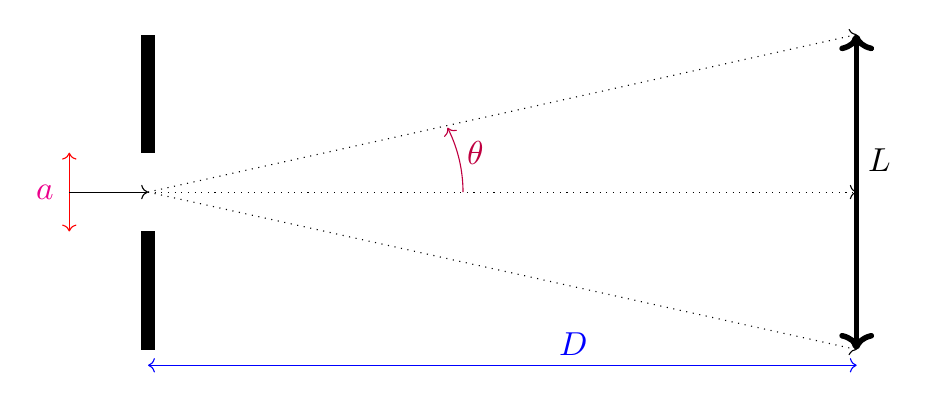
\begin{tikzpicture}
    \draw[black,line width=5pt] (1,-0.5) -- (1,1);
     \draw[black,line width=5pt] (1,-1.5) -- (1,-3);
      \draw[<->, red] (0,-1.5) -- (0,-0.5);
      \node [magenta] (F) at (-0.3,-1) {\large{$a$}};
      \draw[->, black] (0,-1) -- (1,-1);
      \draw[->, black, dotted] (1,-1) -- (10,-1);
      \draw[->, black, dotted] (1,-1) -- (10,1);
       \draw[->, black, dotted] (1,-1) -- (10,-3);
       \draw[<->, black,line width=2pt] (10,-3) -- (10,1) node[right,pos=0.6] {\large{$L$}};;
       \draw[<->, blue] (1,-3.2) -- (10,-3.2) node[above,pos=0.6] {\large{$D$}};
  %    \draw (0,-1) grid  [step=1] (8,5);
  \draw [->,purple] (5,-1) arc (0:27:1.8) node[right,pos=0.6] {\large{$\theta$}};
\end{tikzpicture}
\end{center}

\begin{enumerate}
\def\labelenumi{\arabic{enumi}.}
\setcounter{enumi}{2}
\tightlist
\item
  A la sortie de la fente, estimer l'incertitude \(\delta p_x\) de la
  quantité de mouvement suivant l'axe horizontal de l'onde en fonction
  de la quantité de mouvement \(p\).
\end{enumerate}

\begin{center}
\begin{tikzpicture}

 \draw[black, dashed] (1,0) -- (8,0);
 \draw[->, black, dashed] (1,0) -- (8,5);
 \draw [->,purple] (4,0) arc (0:40:2.5) node[right,pos=0.6] {\large{$\theta$}};
  \draw[->,red] (3,1.4) -- (3,4) node[right=0.18cm,pos=0.6] {\large{$\vec{p_{x}}$}};;;
  \draw[->,red] (3,1.4) -- (6.5,4) node[right=0.3cm,pos=0.6] {\large{$\vec{p}$}};;;
  \draw[->,red, dotted] (3,4) -- (6.5,4) ;
    
\end{tikzpicture}
\end{center}

\begin{enumerate}
\def\labelenumi{\arabic{enumi}.}
\setcounter{enumi}{3}
\tightlist
\item
  Qu'en concluez vous concernant le phénomène de la diffraction ?
\end{enumerate}

\textbf{Solutions :}

\begin{enumerate}
\def\labelenumi{\arabic{enumi}.}
\tightlist
\item
\end{enumerate}

Chaque photon du faisceau laser doit obéir aux règles de la mécanique
quantique, notamment au principe d'incertitude de Heisenberg, qui
stipule qu'il est impossible de connaître à la fois la position et
l'impulsion d'un photon

\[\Delta p_{x} \times \Delta x \geq \frac{\hbar}{2\pi}\]

avec \(\hbar=\frac{h}{2\pi}\)

Si la position est connue avec précision la quantité de mouvement ne
peut être connue de façon précise (et inversement).

\begin{enumerate}
\def\labelenumi{\arabic{enumi}.}
\setcounter{enumi}{1}
\item
  L'incertitude \(\Delta x\) est comparable à la largeur de la fente (la
  fente n'étant pas ponctuelle mais étendue) : \[\Delta x \approx a\]
\item
  Après la fente :
\end{enumerate}

Le sinus d'un angle est le côté opposé sur l'hypoténuse.

\[\sin \theta=\frac {p_{x}}{p}\] La quantite de mouvement avant la fente
était horizontale, l'incertitude sur la quantité de mouvement est
comparable à :

\[\Delta p_{x} = p\ sin \theta -0=p \sin \theta\] 4.
\[\theta \ll 1  \Rightarrow \sin \theta \approx \theta \Rightarrow \Delta p_{x} \approx p \times \Delta \theta\]

En utilisant la relation de De Broglie :

\(p= \frac{h}{\lambda}\Rightarrow \Delta p_{x} \approx \frac {h}{\lambda} \times \Delta \theta\)
(1) si \(\Delta \theta\) indique la gamme des directions

De plus selon le principe d'incertitude :
\(\Delta p_{x} \approx \frac{\hbar}{\Delta x} \approx \frac{\hbar}{a}\)
(2)

De (1) et (2) on tire :

\[\Delta \theta \approx \frac{\lambda}{a}\] Ainsi un faisceau de lumière
parallèle de longueur \(\lambda\) atteingnant une ouverture de taille
caractéristique \(a\) diffracte dans un cone de demi angle au sommet de
l'ordre de \(\frac{\lambda}{a}\), \(\Delta \theta\) indiquant la gamme
de direction empruntée par les photons.

\subsection{6.11 Exercice 3 : Incertitude de
Heisenberg}\label{exercice-3-incertitude-de-heisenberg}

\emph{Source : exercices et problemes resolus de mecaniques quantiques,
Hamid Najib. Exercice 2.4}

\textbf{Questions :}

\begin{enumerate}
\def\labelenumi{\arabic{enumi}.}
\item
  Quelle est l'ordre de grandeur de l'incertitude minimale sur la
  vitesse d'un electron dont la position est déterminée à 0.05
  \(\text{Å}\) près ?
\item
  Dans un état excite l'électron a une durée moyenne de vie de
  \(10^{-8}\) s. Il retourne à son état fondamental en émettant un
  quantum \(h\nu\)
\end{enumerate}

\begin{enumerate}
\def\labelenumi{\alph{enumi}.}
\tightlist
\item
  Calculez l'incertitude minimale sur l'énergie de ce niveau.
\item
  en déduire l'incertitude sur la fréquence et sur la longueur d'onde de
  la radiation émise.
\end{enumerate}

\textbf{Réponses :}

\begin{enumerate}
\def\labelenumi{\arabic{enumi}.}
\tightlist
\item
  1 \(\text{Å}\) = 10\^{}\{-10\} metres.
\end{enumerate}

\Delta x=5.10\^{}\{-12\} metres.

L'incertitude minimale est telle que :

\[\Delta p=\frac{\hbar}{2}\frac{1}{\Delta x}=1.54\times 10^{-23}\]

\(\Delta p=m \times \Delta v\)

\(m_{electron}=9.1.10^{-31}kg\)

\[\Delta v=\frac{1.054.10^{-23}}{9.11.10^{-34}}\]
\(\Delta v=1.16.10^{7} m.s^{-1}\)

\begin{enumerate}
\def\labelenumi{\arabic{enumi}.}
\setcounter{enumi}{1}
\tightlist
\item
  a \[\boxed{\Delta E \times \Delta t \geq \frac{\hbar}{2}}\]
\end{enumerate}

d'ou :

\[\Delta E = \frac{\hbar}{2}\frac{1}{\Delta t}
=\frac{1.05\times10^{-34}}{2}\frac{1}{10^{-8}}=5.2\times 10^{-27} J\]

B. Incertitude sur la frequence :

\[\Delta E=h\Delta \nu\]

\[\Delta \nu=\frac{\Delta E}{h}=\frac{5.2 \times 10^{-27}}{6.6 \times 10^{-34}}=0.78 \times 10^{7} s^{-1}\]
\[\lambda=\frac{c}{\nu}\]

\[\frac{d \lambda}{d \nu}=\frac{d\frac{c}{\nu}}{d\nu}\]

or \[(\frac{1}{x})'=-\frac{1}{x^2}\]

d'ou :

\[d\lambda=\frac{c}{-\nu^2}d\nu\] Toutefois pour faire le calcul il faut
connaitre la valeur de \(\nu\) ?

\subsection{6.14 Exercice 4 : calcul de la TF de la fonction porte
:}\label{exercice-4-calcul-de-la-tf-de-la-fonction-porte}

\emph{Source : Exercices et problèmes résolus de mécanique quantique
Exercice 9.3 page 403} (Najib 2022)

\textbf{Questions :}

Calculer la transformée de Fourier de la fonction porte suivante :

\[\Pi_{a}(x)=\left\{
    \begin{array}{ll}
        1/a & \mbox{pour } |x|<a/2 \\
        0 & \mbox{pour} |x|>a/2
    \end{array}
\right.\]

\begin{figure}
\centering
 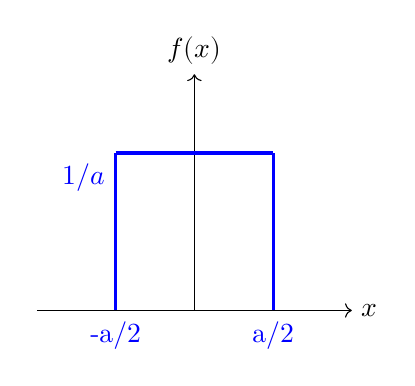
\begin{tikzpicture}
  \draw[->]  (-2,0) node {} -- (2,0)  node[right] {$x$};;
  \draw[->]  (0,0) node {} -- (0,3)  node[above] {$f(x)$};
  \draw[blue, line width=0.04cm]  (-1,0) node[below] {-a/2} -- (-1,2)  node[below left] {$1/a$};
  \draw[blue, line width=0.04cm]  (1,0) node[below] {a/2} -- (1,2)  node[below] {};
   \draw[blue, line width=0.04cm]  (-1,2) node[below] {} -- (1,2)  node[below] {};
\end{tikzpicture}
\end{figure}

\textbf{Solution :}

Tout d'abord partons de la formule de la transformée de fourier :

\[g(k)=\frac{1}{\sqrt{2\pi}} \int_{+\infty}^{-\infty} f(x)e^{-ikx}dx\]
\[g(k)=\frac{1}{\sqrt{2\pi}}\frac{1}{a} \int_{+\infty}^{-\infty} e^{-ikx}dx\]
\[g(k)=\frac{1}{\sqrt{2\pi}}\frac{1}{a} \left[ e^{-ikx}dx \right] _\frac{-a}{2}^\frac{a}{2}  \]
\[g(k)=\frac{1}{\sqrt{2\pi}}\frac{1}{a} ( \frac{1}{- ik}e^{-ik\frac{a}{2}} -\frac{1}{-ik}e^{ik\frac{a}{2}}) \]
\[g(k)=\frac{1}{\sqrt{2\pi}}\frac{1}{a}  \frac{1}{-ik}(e^{-ik\frac{a}{2}} -e^{ik\frac{a}{2}})\]

Valeur de \(e^{-i\theta} - e^{i\theta}\)

Selon les formules d'Euler, on a
\[e^{i\theta} = \cos \theta + i \sin \theta\] et
\[e^{-i\theta} = \cos \theta - i \sin \theta\]. En soustrayant, on
obtient
\[e^{-i\theta} - e^{i\theta} = (\cos \theta - i \sin \theta) - (\cos \theta + i \sin \theta) = -2i \sin \theta\].
Donc, \[e^{-i\theta} - e^{i\theta} = -2i \sin \theta\].

On obtient donc :

\[\frac{1}{\sqrt{2\pi}}\frac{1}{a}  \frac{1}{-ik} -2i\sin(k\frac{a}{2})\]

En simplifiant par i et le 2 passe en desous on obtient :

\[g(k)=\frac{1}{\sqrt{2\pi}}\frac{1}{\frac{ka}{2}} \sin(\frac{ka}{2})\]
C'est une fonction sinus cardinal de type
\(sinc(x) = (\frac{\sin x}{x})\)

\subsection{6.17 Exercice 5 : paquet d'onde Gaussien
:}\label{exercice-5-paquet-donde-gaussien}

\emph{Source : Exercices et problèmes résolus de mécanique quantique:
Avec rappels de cours} (Najib 2022)

On donne a l'instant t=0 le paquet d'onde représentant le mouvement
d'une particule libre, de masse m :

\[\Phi(x,0)=\frac{1}{\sqrt{2\pi}}\int_{-\infty}^{+\infty} g(k)e^{ikx}dk\]
avec
\[g(k)=\frac{\sqrt{a}}{(2\pi)^\frac{1}{4}}e^{\frac{{{-a^2}(k-k_(0))^2}}{4}}\]

et :

\(k_{0}=\frac{2\pi}{\lambda_{0}}\);\(k=\frac{2\pi}{\lambda}\)

\(a\) est une constante réelle; \(\lambda_{0}\) est la longueur d'onde
autour de laquelle se repartissent les différentes longueurs d'onde
\(\lambda\) du paquet.

\begin{center}
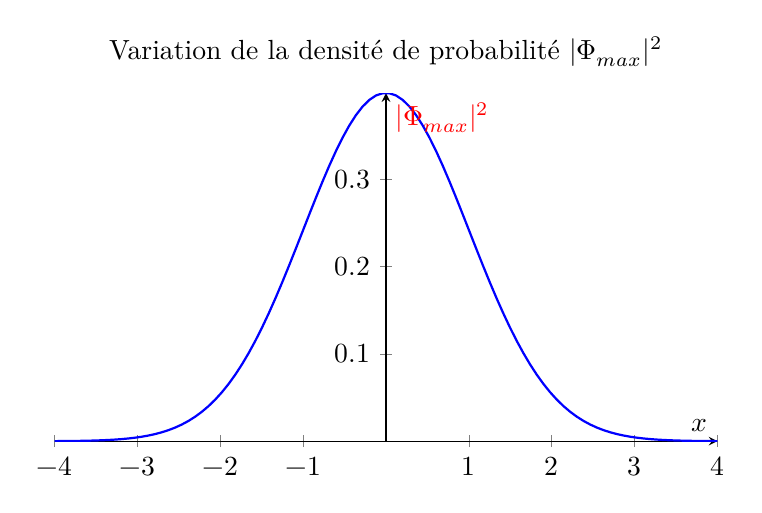
\begin{tikzpicture}
  \begin{axis}[
    domain=-4:4,
    samples=100,
    axis lines=middle,
    xlabel=$x$,
    ylabel={\textcolor{red}{$|\Phi_{max}|^2$}},
    height=6cm,
    width=10cm,
    title={Variation de la densité de probabilité $|\Phi_{max}|^2$}
  ]
    \addplot [
      thick,
      blue
    ] {1/sqrt(2*pi) * exp(-x^2/2)};
  \end{axis}
\end{tikzpicture}
\end{center}

\begin{enumerate}
\def\labelenumi{\arabic{enumi}.}
\tightlist
\item
\end{enumerate}

\begin{enumerate}
\def\labelenumi{\alph{enumi}.}
\tightlist
\item
  Calculer \(\Phi(x,0)\) en fonction de a, k\_\{0\} et x.
\end{enumerate}

Définition de la fonction \(\phi(x,0)\) pour une onde de Fourier d'un
état initial La fonction donnée est :
\[ \phi(x,0) = \frac{1}{\sqrt{2\pi}} \int_{-\infty}^{+\infty} \frac{\sqrt{a}}{(2\pi)^{1/4}} e^{-\frac{a^2 (k - k0)^2}{4}} e^{i k x} , dk \]

Analyse de la forme de \(\phi(x,0)\) Il s'agit d'une transformée de
Fourier de la fonction :
\[ \hat{\phi}(k) = g(k)= \frac{\sqrt{a}}{(2\pi)^{1/4}} e^{-\frac{a^2 (k - k_0)^2}{4}} \]

Origine de \[\hat{\phi}(k)\]

La fonction \(\hat{\phi}(k)\) est une gaussienne centrée en \(k_{0}\),
de largeur proportionnelle à \(1/a\). La transformée de Fourier d'une
gaussienne est une autre gaussienne, ce qui explique la forme de
\(\hat{\phi}(k)\). 2. Expression de \(\phi(x,0)\) La fonction
\(\phi(x,0)\) est la transformée inverse de \(\hat{\phi}(k))\), ce qui
donne :
\[\phi(x,0) = \frac{1}{\sqrt{2\pi}} \int_{-\infty}^{+\infty} \hat{\phi}(k) e^{i k x} , dk\]
Ici, \(\hat{\phi}(k))\) est une gaussienne centrée en \(k_{0}\).

\emph{Calcul explicite}

La transformée inverse d'une gaussienne est une autre gaussienne :
\[\phi(x,0) = \frac{1}{\sqrt{2\pi}} \times \frac{\sqrt{a}}{(2\pi)^{1/4}} \int_{-\infty}^{+\infty}e^{-\frac{a^2 (k - k0)^2}{4}} e^{i k x} , dk\]
En effectuant le changement de variable \(k' = k - k_{0}\), on obtient :
\[ \phi(x,0) = \frac{1}{\sqrt{2\pi}} \times \frac{\sqrt{a}}{(2\pi)^{1/4}} e^{ik_{0}x} \int_{-\infty}^{+\infty} e^{-\frac{a^2 k'^2}{4}} e^{i k' x} , dk'\]

La transformée de Fourier d'une gaussienne est une autre gaussienne :

\[ \int_{-\infty}^{+\infty} e^{-\alpha k'^2} e^{i \beta k'} , dk' = \sqrt{\frac{\pi}{\alpha}} e^{-\frac{\beta^2}{4 \alpha}} \]

Ici, \(\alpha = \frac{a^2}{4}\) et \(\beta = x\). Donc :
\[ \int_{-\infty}^{+\infty} e^{-\frac{a^2}{4} k'^2} e^{i k' x} , dk' = \sqrt{\frac{\pi}{a^2/4}} e^{-\frac{x^2}{a^2}} = \frac{2 \sqrt{\pi}}{a} e^{-\frac{x^2}{a^2}} \]
\emph{Resultat final:} En rassemblant tous les termes, on obtient :
\[\phi(x,0) = \frac{1}{\sqrt{2\pi}} \times \frac{\sqrt{a}}{(2\pi)^{1/4}} e^{i k_0 x} \times \frac{2 \sqrt{\pi}}{a} e^{-\frac{x^2}{a^2}}\]
\emph{Simplifions le facteur numérique :}

\[\phi(x,0) = \left( \frac{1}{\sqrt{2\pi}} \times \frac{\sqrt{a}}{(2\pi)^{1/4}} \times \frac{2 \sqrt{\pi}}{a} \right) e^{i k_0 x} e^{-\frac{x^2}{a^2}}\]

\emph{Calculons le coefficient :}

\[ \frac{1}{\sqrt{2\pi}} \times \frac{\sqrt{a}}{(2\pi)^{1/4}} \times \frac{2 \sqrt{\pi}}{a} \]

\emph{Conclusion}
\[ \boxed{ \phi(x,0) = {\frac{2}{\pi \times a^2} ^{1/4}} e^{i k_0 x} e^{-\frac{x^2}{a^2}} } \]

Ce résultat montre que l'état initial est une gaussienne centrée en
(x=0), modulée par une phase oscillante \(e^{i k_{0} x}\), avec une
largeur contrôlée par \(a\).

Résumé : La fonction \(\phi(x,0)\) est la transformée inverse de la
gaussienne \(\hat{\phi}(k)\), qui est une distribution de Fourier d'une
gaussienne centrée en \(k_{0}\). La forme finale est une gaussienne en
\(x\), avec une phase oscillante, et un facteur numérique dépendant de
\(a\).

\emph{Rappel :}

Une phase oscillante \(e^{i k_{0}x}\) est une expression mathématique
utilisée pour représenter une onde ou une perturbation qui se propage
dans l'espace. Elle décrit une variation harmonique de la phase de
l'onde en fonction de la position \(x\).

\emph{Explication :}

\(e^{i k_0 x}\) est une fonction complexe, où :

\(i\) est l'unité imaginaire \(i^2 = -1\), \(k_0\) est la constante de
propagation ou nombre d'onde, qui indique la fréquence spatiale de
l'oscillation (en radian par mètre, \(x\) est la position dans l'espace.
La partie réelle de cette expression, généralement \(\cos(k_{0}x\),
représente une onde sinusoïdale en termes de phase, tandis que la partie
imaginaire \(\sin(k_{0}x)\) représente la composante sinusoïdale
déphasée.

\emph{Interprétation physique :}

La phase de l'onde à une position \(x\) est donnée par
\(\phi(x) = k_{0} x\). Cela signifie que la phase de l'oscillation varie
linéairement avec la position. La propagation de l'onde se traduit par
une variation de cette phase, permettant de décrire la direction et la
vitesse de déplacement de l'onde dans l'espace.

\begin{enumerate}
\def\labelenumi{\alph{enumi}.}
\setcounter{enumi}{1}
\tightlist
\item
  Représenter à \(t=0\) la forme du paquet d'onde c'est a dire la
  variation de la densité de probabilité de localisation de la
  particule; On montrera que c est une gaussienne.
\end{enumerate}

La fonction donnée est :
\[\phi(x,0) = \left( \frac{2}{\pi \times a^2} \right)^{1/4} e^{i k_0 x} e^{-\frac{x^2}{a^2} } \]

Interprétation Cette expression correspond à une fonction d'onde en
mécanique quantique, souvent utilisée pour représenter l'état initial
d'une particule. Elle combine une composante gaussienne, caractéristique
d'une distribution de position, avec une phase oscillante, liée à la
quantité de mouvement.

Analyse de la densité de probabilité La densité de probabilité associée
à une fonction d'onde \(\phi(x,0)\) est donnée par le module au carré de
cette fonction :

\[|\phi(x,0)|^2 = \phi(x,0) \times \phi^*(x,0)\]

où \(\phi^*(x,0)\) est le complexe conjugué de \(\phi(x,0)\).

La phase \(e^{i k_0 x}\) disparaît lors du calcul du module au carré,
car :

\[|e^{i k_0 x}|^2 = e^{i k0 x} \times e^{-i k0 x} = 1\]

La densité de probabilité devient alors :

\[
|\phi(x,0)|^2 = \left( \frac{2}{\pi a^2} \right)^{1/2} e^{-\frac{2 x^2}{a^2}}\]

Conclusion La densité de probabilité de la particule à l'instant initial
est une distribution gaussienne centrée en \(x=0\), avec une largeur
caractérisée par le paramètre \(a\). Elle s'exprime donc comme :
\[ \boxed{ |\phi(x,0)|^2 = \left( \frac{2}{\pi a^2} \right)^{1/2} e^{-\frac{2 x^2}{a^2}}
} \]

Ce résultat indique que la probabilité de trouver la particule en un
point \(x\) est donnée par une distribution normale avec une moyenne
nulle et une variance \[\sigma^2 = \frac{a^2}{4}\].

Remarque : La phase \(e^{i k0 x}\) ne modifie pas la densité de
probabilité, mais elle indique une impulsion moyenne non nulle,
correspondant à une quantité de mouvement moyenne \(p0 = \hbar k_0\).

\begin{enumerate}
\def\labelenumi{\alph{enumi}.}
\setcounter{enumi}{2}
\tightlist
\item
  Déterminer la largueur a mi-hauteur \(\Delta x\) du paquet d'onde dans
  l'espace des configurations \{x\}.
\end{enumerate}

La fonction donnée est une distribution gaussienne de la forme :
\[ |\phi(x,0)|^2 = \left( \frac{2}{\pi a^2} \right)^{1/2} e^{-\frac{2 x^2}{a^2}} \]

En comparant, on peut supposer que la fonction est une gaussienne
centrée en 0 avec une largeur caractéristique liée à \(a\).

Relation entre largeur à mi-hauteur et écart-type pour une gaussienne
Pour une distribution gaussienne de la forme :
\[ f(x) = A e^{-\frac{x^2}{2\sigma^2}} \]

La largeur à mi-hauteur (FWHM) est donnée par :
\[ \text{FWHM} = 2 \sqrt{2 \ln 2} \times  \sigma \]

Application à la fonction donnée Dans l'expression fournie,
l'exponentielle est : \[ e^{-\frac{2 x^2}{a^2}} \]

Elle peut être réécrite sous la forme : \[ e^{-\frac{x^2}{2\sigma^2}} \]

en identifiant :
\[ \frac{1}{2\sigma^2} = \frac{2}{a^2} \Rightarrow \sigma^2 = \frac{a^2}{4} \Rightarrow \sigma = \frac{a}{2} \]

Calcul de la largeur à mi-hauteur Donc, la FWHM est :
\[ \text{FWHM} = 2 \sqrt{2 \ln 2} \times \frac{a}{2} = \sqrt{2 \ln 2} \times a \]

Résultat final La largeur à mi-hauteur de la fonction est :
\[ \boxed{\text{FWHM} = a \times \sqrt{2 \ln 2} \approx 1.177 \times a} \]

Ce résultat indique que la largeur à mi-hauteur est proportionnelle à la
paramètre (a), avec un facteur d'environ 1.177.

\begin{enumerate}
\def\labelenumi{\alph{enumi}.}
\setcounter{enumi}{3}
\tightlist
\item
  Déterminer à partir de la transformée de fourier de la fonction
  \(\Phi(x,0)\), la largeur à mi-hauteur \(\Delta k\) dans l'espace des
  configurations \{k\}.
\end{enumerate}

\[|g(k)|^2=\frac{a}{\sqrt{2\pi}}
e^{\frac{-a^2(k-k_{0})^2}{2}}\]

La fonction fournie est une distribution gaussienne en (k) de la forme :

\[
|g(k)|^2 = \frac{a}{\sqrt{2\pi}} , e^{-\frac{a^2 (k - k_0)^2}{2}}
\]

où :

a est un paramètre positif, \(k_{0}\) est la position du pic.

Étape 1 : Identifier la valeur maximale La valeur maximale de cette
fonction est atteinte en \(k = k_{0}\) :

\[|g(k_0)|^2 =\frac{a}{\sqrt{2\pi}}\]

Étape 2 : Définir la largeur à mi-hauteur La largeur à mi-hauteur
\(FWHM\) correspond à la différence entre les deux valeurs de \(k\) pour
lesquelles :

\[
|g(k)|^2 = \frac{1}{2} \times |g(k_0)|^2
\]

Donc, on cherche (k) tel que :

\[ \frac{a}{\sqrt{2\pi}} e^{-\frac{a^2 (k - k_0)^2}{2}} = \frac{1}{2} \times \frac{a}{\sqrt{2\pi}} \]

Ce qui simplifie à :

\[ e^{-\frac{a^2 (k - k_0)^2}{2}} = \frac{1}{2} \]

Étape 3 : Résoudre pour \[\Delta k = |k - k_0|\] Prenons le logarithme
naturel des deux côtés :

\[ -\frac{a^2 (k - k_0)^2}{2} = \ln \left( \frac{1}{2} \right) = -\ln 2 \]

rapel :pour tout ( a \textgreater{} 0 ) et ( b \textgreater{} 0 ), on a
:

\[ \ln \left( \frac{a}{b} \right) = \ln a - \ln b \]

En appliquant cette propriété avec ( a = 1 ) et ( b = 2 ), on obtient :

\[ \ln \left( \frac{1}{2} \right) = \ln 1 - \ln 2 \]

Sachant que \(\ln 1 = 0\) , car le logarithme naturel de 1 est toujours
0, on a :

\[ \ln \left( \frac{1}{2} \right) = 0 - \ln 2 = - \ln 2 \]

Ce qui donne :

\[ a^2 (k - k_0)^2 = 2 \ln 2 \]

Donc :

\[
|k - k_0| = \frac{\sqrt{2 \ln 2}}{a}
\]

Conclusion : La largeur à mi-hauteur (FWHM) est donc :

\[ \boxed{ \text{FWHM} = 2 \times |k - k_0| = 2 \times \frac{\sqrt{2 \ln 2}}{a} = \frac{2 \sqrt{2 \ln 2}}{a} } \]

Résumé : La largeur à mi-hauteur de la distribution \[ |g(k)|^2 \] est :
\[ \boxed{ \text{FWHM} = \frac{2 \sqrt{2 \ln 2}}{a} } \]

Elle est inversement proportionnelle au paramètre (a).

\begin{enumerate}
\def\labelenumi{\alph{enumi}.}
\setcounter{enumi}{4}
\tightlist
\item
  Vérifier que le principe d'incertitude d'Heisenberg est satisfait.
\end{enumerate}

\[\Delta x.\Delta k=4\ln2 > \frac{1}{2}\]

\begin{enumerate}
\def\labelenumi{\alph{enumi}.}
\setcounter{enumi}{5}
\tightlist
\item
  Calculer la fonction \(\Phi(x,t)\) pour tout instant t sachant que la
  pulsation est donnée par la relation de dispersion des ondes de Louis
  de Broglie : \(\omega=\frac{hbar}{2m}k^2\)
\end{enumerate}

Transformation de \(\phi(x,0)\) en \(\phi(x,t)\) pour un paquet d'onde
gaussien Pour faire évoluer une fonction d'onde initiale \(\phi(x,0)\),
notamment un paquet d'onde gaussien, en une fonction d'onde à un instant
ultérieur \(t\), on utilise la représentation en ondes planes et la
transformée de Fourier.

Étapes de la transformation Expression initiale en Fourier : La fonction
d'onde initiale \(\phi(x,0)\) peut être exprimée comme une superposition
d'ondes planes via sa transformée de Fourier \(\tilde{\phi}(k)\) :

\[\phi(x,0) = \frac{1}{\sqrt{2\pi}} \int_{-\infty}^{+\infty} \tilde{\phi}(k) e^{i k x} , dk \]
où \(\tilde{\phi}(k)\) est la transformée de Fourier de \(\phi(x,0)\).

Transformation en fonction du temps : Dans le cas d'une particule libre,
chaque onde plane évolue selon la phase

\[ e^{i(kx - \omega t)}\], avec \[\omega = \frac{\hbar k^2}{2m}\]

(pour une particule libre). La fonction d'onde à l'instant \(t\) est
donc donnée par :

\[ \phi(x,t) = \frac{1}{\sqrt{2\pi}} \int_{-\infty}^{+\infty} \tilde{\phi}(k) e^{i(k x - \omega t)} , dk \]

en remplaçant \(\omega\) par sa valeur spécifique pour une particule
libre.

Expression finale : La transformation temporelle de \(\phi(x,0))\) en
\((\phi(x,t))\)\$ s'écrit donc :

\[\boxed{ \phi(x,t) = \frac{1}{\sqrt{2\pi}} \int_{-\infty}^{+\infty} {g}(k) e^{i k x} e^{-i \frac{\hbar k^2}{2m} t} , dk } \]

On pose : \[\lambda=\frac{\hbar t}{2m}\]

\emph{Rappel :} Dans le contexte de la mécanique quantique, la longueur
d'onde associée à une particule, notamment la longueur d'onde de de
Broglie, est généralement donnée par \(\lambda = \frac{h}{p}\), où p est
la quantité de mouvement. La constante réduite
\(\hbar = \frac{h}{2\pi}\) intervient souvent dans les calculs liés aux
phénomènes ondulatoires.

Cependant, la formule \(\lambda = \frac{\hbar t}{2m}\) ne correspond pas
directement à une expression standard dans la mécanique quantique ou la
mécanique ondulatoire. Elle pourrait faire référence à une relation
spécifique dans un contexte particulier, par exemple, la largeur d'une
onde ou la propagation d'une onde de wave packet, ou encore une
approximation dans un problème de diffusion ou de propagation libre.

On obtient ainsi :

\[\boxed{ \frac{1}{\sqrt{2}{\pi}} \frac{\sqrt(a)}{2\pi^{\frac{1}{4}}} \int_{-\infty}^{+\infty} {g}(k) e^{i k x} e^{-i \frac{\hbar k^2}{2m} t} , dk } \]

puis :

\[\psi(x,\lambda)=\frac{1}{\sqrt{2\pi}} \frac{\sqrt{a}}{2\pi^{\frac{1}{4}}}\int_{-\infty}^{+\infty}  e^{ -\frac{{a^2}(k-k_{0})^2}{4}+ikx-i\lambda k^2} dk\]

\begin{enumerate}
\def\labelenumi{\alph{enumi}.}
\setcounter{enumi}{6}
\tightlist
\item
  Justifier sans calcul pourquoi \(\Phi(x,t)\) est solution de
  l'équation de Schrödinger.
\end{enumerate}

Puisque la fonction d'onde de L de Broglie est solution de l'équation de
schrodinger, le paquet d'onde qui est une combinaison linéaire de
fonctions de type onde de De Broglie est donc solution de cette
équation.

\begin{enumerate}
\def\labelenumi{\alph{enumi}.}
\setcounter{enumi}{7}
\tightlist
\item
  Montrer que le paquet d'onde s'étale dans le temps. On discutera la
  densité de probabilité et on déterminera la vitesse de groupe
  \(v_{g}\)
\end{enumerate}

a faire

On donne :
\[\int_{-\infty}^{+\infty} e^{-\gamma z^2+i\eta z} dz=\frac{\sqrt{\pi}}{\sqrt{|\gamma|}}e^{\frac{-\eta^2}{4\gamma}}\]

\(\frac{-\pi}{4} < arg(\gamma) < \frac{\pi}{4}\)

\subsection{8.1 Exercice 6 : le puits de potentiel
infini}\label{exercice-6-le-puits-de-potentiel-infini}

Source : \emph{exercice et problèmes résolus de mécanique quantique.
Exercice 3.5 page 79 (examen filière mathématique physique deuxième
année. Kenitra, juin 2003)} (Najib 2022)

On considère un problème à une dimension correspondant à une particule
de masse m et d'énergie E, placée dans un puit de potentiel infini de
largeur a :

\[V(x)= \left\{
    \begin{array}{ll}
        0 & \mbox{si } -a \leq x \leq 0 \\
        +\infty & \mbox{ailleurs}
    \end{array}
\right.\]

\usetikzlibrary{patterns}
\begin{figure}
\centering
 \begin{tikzpicture}
  \draw[->]  (-3,0) node {} -- (3,0)  node[right] {$x$};;
  \draw[->]  (1,0) node {} -- (1,3)  node[above] {$V(x)$};
  \draw[blue, line width=0.04cm]  (-1,0) node[below] {-a} -- (-1,2.5)  node[left] {};
  \draw[blue, line width=0.04cm]  (1,0) node[below] {0} -- (1,2.5)  node[below] {};
%   \draw[blue, line width=0.04cm]  (-1,2) node[below] {} -- (1,2)  node[below] {};
 \fill[pattern=horizontal lines, pattern color=gray!50] (-1,0) rectangle (-3,3);
  \fill[pattern=horizontal lines, pattern color=gray!50] (1,0) rectangle (3,3);
   \node[red] at (-2,1.5) {(I)};
    \node[red] at (0,1.5) {(II)};
     \node[red] at (2,1.5) {(III)};
\end{tikzpicture}
\end{figure}

Soit \(\cal H\) l'hamiltonien de la particule et soit \(\Psi(x,t)\) sa
fonction d'onde associee.

\begin{enumerate}
\def\labelenumi{\arabic{enumi}.}
\tightlist
\item
  Écrire et résoudre l'équation de schrodinger indépendante du temps
  pour chacune des régions d'espace \((I)\), \((II)\) et \((III)\).
\end{enumerate}

\textbf{Réponse :}

On posera :

\[k=\sqrt{\frac{2m}{\hbar^2}E}\] et on donnera la forme générale des
fonctions d'onde d'état stationnaire de la particule.

Voici l'équation de Schrodinger indépendante du temps :
\[[\frac{d^2}{dx^2} + \frac{2m}{\hbar}(E-V(x))]\phi(x)=0\] Dans les
zones I et III le potentiel est infini donc la particule ne pénètre
jamais. \(\phi(x)=0\)

Dans la zone II, on doit se ramener a une équation de la forme :

\[ay''+by'+cy=0\] De plus V(x)=0

On presence note équation sous une forme plus claire :

\[\frac{d^2}{dx^2}\phi(x) + (\frac{2m}{\hbar}E)\phi(x)=0\] Ainsi on pose
:

\(b=0\), \(a=1\) et \(c=\frac{2m}{\hbar^2}E\)

\[\Delta=b^2 -4ac=0-4.1.\frac{2m}{\hbar^2}E\] avec \(\Delta < 0\)

On a donc des solutions sous forme complexe conjuguee :

\[r1=\frac{-b +\sqrt{\Delta}}{2a}\] \[r1=\frac{-b -\sqrt{\Delta}}{2a}\]
Je vous laisse faire le calcul.

on obtient : \(r1=ik\) \(r2=-ik\)

avec \[k=\sqrt{\frac{2m}{\hbar}}E\]

La fonction d'onde a donc pour forme :

\[\phi_{II}(x)=Ce^{ikx} + De^{-ikx}\]

\begin{enumerate}
\def\labelenumi{\arabic{enumi}.}
\setcounter{enumi}{1}
\tightlist
\item
  Ecrire les conditions de continuite des fonctions propres de
  \(\cal H\) et montrer aue les valeurs propres \(E_{n}\) (n entier)
  correspondantes sont quantifiées.
\end{enumerate}

\textbf{Réponse :}

Voici les conditions aux limites :

\(\phi_{II}(0)=0\)

\(\phi_{II}(a)=0\)

Comme \[\phi_{II}(x)=Ce^{ikx} + De^{-ikx}\]

\(\phi_{II}(0)=C+D=0\)

Donc \(C=-D\)

Appliquons la seconde condition :

\[\phi_{II}(a)=Ce^{ika} + De^{-ika}\]
\[\phi_{II}(a)=C(\cos ka +i\sin ka) + (D\cos ka -i\sin ka)\] Comme C=-D
les termes en cosinus s'annulent.

\[\phi_{II}(a)=-Di\sin ka -Di\sin ka=0\]

\[-2Di\sin ka=0\] \[\boxed{\phi_{II}(x)=2iCsin(\frac{n\pi}{a}x)}\]

D n'etant pas nul, \[ka=n\pi\]

De plus,

\[k=\sqrt{\frac{2m}{\hbar^2}E}\]

En remplacant k dans l'expression on obtient :

\[\boxed{E_{n}=\frac{n^2\pi^2}{a^2}\frac{\hbar}{2m}}\]

\begin{enumerate}
\def\labelenumi{\arabic{enumi}.}
\setcounter{enumi}{2}
\tightlist
\item
  En déduire la fonction propre normalisée à l'unité correspondant à
  l'énergie propre \(E_{n}\).
\end{enumerate}

\textbf{Réponse :}

La constante F est déterminée en normalisation la fonction d'onde a
l'unité:

\[\int_{-a}^{0}|\phi(x)|^2=|F|^2\int_{-a}^{0}\sin^2(\frac{n\pi}{a}x)dx=1\]

Le problème est qu'il faut calculer la primitive d'un \(sin^2\)

Procédons à un changement de variable :

\(t=\frac{n\pi}{a}x\)

\(x=\frac{ta}{n\pi}\)

\(dx=\frac{a}{n\pi}dt\)

On obtient :

\[\int_{-a}^{0}\sin^2(\frac{n\pi}{a}x)dx=\frac{a}{n\pi}\int_{-n\pi}^{0}\sin^2(t)dt\]
Or \(\sin^2(x)=\frac{(1-cos2x}{2}\)

\[\frac{a}{n\pi}\int_{-n\pi}^{0}\sin^2(t)dt=\]
\[\frac{a}{n\pi}\int_{-n\pi}^{0}\frac{1-cos2t}{2}dt=\]
\[\frac{a}{n\pi}\int_{-n\pi}^{0}\frac{1}{2}dt-\frac{a}{n\pi}\int_{-n\pi}^{0}\frac{-cos2t}{2}dt=\]
\[\frac{a}{n\pi}(\left[\frac{1}{2}\right]_{-n\pi}^0+\frac{1}{2}\left[sin2t\right]_{-n\pi}^0)=\]
\[\frac{a}{n\pi}\frac{n\pi}{2}=\frac{a}{2}=\frac{1}{|F|^2}\] On en
deduit que \(F=\sqrt{2}{a}\)

\[\Phi_{n}(x)=\sqrt\frac{2}{a}\sin(\frac{n\pi}{a}x)\] et
\[\Psi(x,t)=\sqrt{\frac{2}{a}}\sin(\frac{n\pi}{a}x)e^{\frac{-iEnt}{\hbar}}\]
avec \[E_{n}=\frac{n^2\pi^2}{a^2}\frac{\hbar}{2m}\]

\begin{enumerate}
\def\labelenumi{\arabic{enumi}.}
\setcounter{enumi}{3}
\tightlist
\item
  A l'instant t=0 la particule a pour fonction d'onde :
\end{enumerate}

\[\psi(x,0)=\frac{1}{\sqrt{a}}[sin{\frac{\pi x}{a}}+sin{\frac{2\pi x}{a}}]\]
dans 'intervalle {[}-a, 0{]}.

\begin{enumerate}
\def\labelenumi{\alph{enumi}.}
\item
  Calculer \(\psi(x,t)\) et sa norme.
\item
  Montrer que la densité de probabilité de présence de la particule
  dépend de la fréquence de Bohr \(\nu_{21}\) dont on précisera
  l'expression en fonction de \(m\), \(a\) et \(\hbar\). Interpréter ce
  résultat.
\end{enumerate}

\subsection{12.2 Exercice 8 : cas d'usage : spécification d'un réseau
décentralisé en utilisant les technologies quantiques
:}\label{exercice-8-cas-dusage-spuxe9cification-dun-ruxe9seau-duxe9centralisuxe9-en-utilisant-les-technologies-quantiques}

Objet du problème : dans le domaine de l'énergie, il est nécessaire
d'utiliser des réseaux décentralisés pour des raisons de sécurité.

Question : Peut-on utiliser la quantique pour améliorer la
décentralisation de la distribution d'électricité ? Quelles offres
existent aujourd'hui ? Quelle est la maturité des solutions ?

\section*{Références :}\label{ruxe9fuxe9rences}
\addcontentsline{toc}{section}{Références :}

\phantomsection\label{refs}
\begin{CSLReferences}{1}{0}
\bibitem[\citeproctext]{ref-aspect:tel-00011844}
Aspect, Alain. 1983. {``{Trois tests exp{é}rimentaux des in{é}galit{é}s
de Bell par corr{é}lation de polarisation de photons}.''} Theses,
{Universit{é} Paris Sud - Paris XI}.
\url{https://pastel.hal.science/tel-00011844}.

\bibitem[\citeproctext]{ref-alma991002711819705804}
Blaquière, Augustin. 1960. \emph{Calcul Matriciel / Austin
Blaquière,.... Tome II. Application à La Mécanique Quantique}.
Classiques Hachette. Paris: Hachette.

\bibitem[\citeproctext]{ref-alma991002711779705804}
Blaquière, Augustin, and Debiesse Jean. 1960. \emph{Calcul Matriciel /
Austin Blaquière,... ; {[}Introduction de j. Debiesse,...{]}. Tome i.
Application à La Physique}. Classiques Hachette. Paris: Hachette.

\bibitem[\citeproctext]{ref-BOHR1928}
BOHR, N. 1928. {``The Quantum Postulate and the Recent Development of
Atomic Theory1.''} \emph{Nature} 121 (3050): 580--90.
\url{https://doi.org/10.1038/121580a0}.

\bibitem[\citeproctext]{ref-bortzmeyerBlogStxE9phane}
Bortzmeyer, Stephane. {``{B}log {S}tephane {B}ortzmeyer: {L}a Securite
de {T}{C}{P}: Plein de Nouveaux {R}{F}{C} Depuis Trois Ans ---
Bortzmeyer.org.''} \url{https://www.bortzmeyer.org/tcp-security.html}.

\bibitem[\citeproctext]{ref-debroglie:tel-00006807}
Broglie, Louis de. 1924. {``{Recherches sur la th{é}orie des Quanta}.''}
Theses. \url{https://theses.hal.science/tel-00006807}.

\bibitem[\citeproctext]{ref-Carpentier2022-nn}
Carpentier, Renaud, and Benoı̂t Depret. 2022. \emph{La Physique En
Applications: 140 Probl{è}mes Corrig{é}s Contemporains
{PC-MP-PMI-PSI-PT}}.

\bibitem[\citeproctext]{ref-Chevoir2013-fq}
Chevoir, François. 2013. \emph{Physique Statistique Pour l'ing{é}nieur:
Cours de l'{É}cole Des Ponts}. Presses Ponts et Chauss{é}es.

\bibitem[\citeproctext]{ref-cluzel:hal-04052636}
Cluzel, Thomas, Claude Mazel, and David R. C. Hill. 2020.
{``{D{é}couverte de l'informatique quantique, {é}tat de l'art et tests
sur machine IBM}.''} {LIMOS}.
\url{https://uca.hal.science/hal-04052636}.

\bibitem[\citeproctext]{ref-PHSC_2001__5_1_105_0}
Coret, André. 2001. {``Un Pas Décisif Vers La Théorie Quantique~:
L'article de Heisenberg de 1925.''} \emph{Philosophia Scientiae} 5:
105--41. \url{http://dml.mathdoc.fr/item/PHSC_2001__5_1_105_0}.

\bibitem[\citeproctext]{ref-Degiovanni2020-yq}
Degiovanni, Pascal, Natacha Portier, Clément Cabart, Alexandre Feller,
and Benjamin Roussel. 2020. \emph{Physique Quantique, Information Et
Calcul}. Savoirs Actuels. EDP Sciences.

\bibitem[\citeproctext]{ref-Delbarre2022-bb}
Delbarre, Delphine, and Marie Warembourg. 2022. \emph{R{é}ussir En
Physique Dans Le Sup{é}rieur: Les Outils Math{é}matiques
Indispensables}.

\bibitem[\citeproctext]{ref-Dixneuf2007-oc}
Dixneuf, Daniel, and Fabien Bellouvet. 2007. \emph{Principes Des
Circuits {é}lectriques: Cours Et Exercices Corrig{é}s}.

\bibitem[\citeproctext]{ref-Einstein1905-zf}
Einstein, A. 1905. {``{Ü}ber Einen Die Erzeugung Und Verwandlung Des
Lichtes Betreffenden Heuristischen Gesichtspunkt.''} \emph{Ann. Phys.}
322 (6): 132--48.

\bibitem[\citeproctext]{ref-gheorghiu:hal-02164412}
Gheorghiu, Alexandru, Theodoros Kapourniotis, and Elham Kashefi. 2019.
{``{Verification of Quantum Computation: An Overview of Existing
Approaches}.''} \emph{{Theory of Computing Systems}} 63 (4): 715--808.
\url{https://doi.org/10.1007/s00224-018-9872-3}.

\bibitem[\citeproctext]{ref-Greiner2009-sw}
Greiner, Walter. 2009. \emph{M{é}canique Quantique. Une Introduction}.
1999th ed. Berlin, Germany: Springer.

\bibitem[\citeproctext]{ref-Heisenberg1925}
Heisenberg, W. 1925. {``�Ber Quantentheoretische Umdeutung Kinematischer
Und Mechanischer Beziehungen.''} \emph{Zeitschrift f�r Physik} 33 (1):
879--93. \url{https://doi.org/10.1007/bf01328377}.

\bibitem[\citeproctext]{ref-london1939theorie}
London, F., and E. Bauer. 1939. \emph{La Th{é}orie de l'observation En
m{é}canique Quantique, Par f. London Et e. Bauer}. Expos{é}s de Physique
g{é}n{é}ral. Hermann.
\url{https://books.google.fr/books?id=Py_BtAEACAAJ}.

\bibitem[\citeproctext]{ref-Najib2022-qq}
Najib, Hamid. 2022. \emph{Exercices Et Probl{è}mes r{é}solus de
m{é}canique Quantique: Avec Rappels de Cours}. Editions Ellipses.

\bibitem[\citeproctext]{ref-Perez2013-it}
Perez, José-Philippe, Robert Carles, and Olivier Pujol. 2013.
\emph{Quantique, Fondements Et Applications: Avec 250 Exercices Et
Probl{è}mes r{é}solus}. De Boeck Sup{é}rieur.

\bibitem[\citeproctext]{ref-Planck1901-fc}
Planck, Max. 1901. {``Ueber Das Gesetz Der Energieverteilung Im
Normalspectrum.''} \emph{Ann. Phys.} 309 (3): 553--63.

\bibitem[\citeproctext]{ref-Schrodinger1926-vy}
Schrödinger, E. 1926. {``Quantisierung Als Eigenwertproblem.''}
\emph{Ann. Phys.} 384 (4): 361--76.

\bibitem[\citeproctext]{ref-Poincaruxe9Seminar2021ITPS}
Seminar, Poincaré, Bertrand Duplantier, Vincent Rivasseau, Bertrand
Duplantier, and Vincent Rivasseau. 2021. \emph{Information Theory:
Poincaré Seminar 2018}. 1st Edition 2021. Vol. 78. Progress in
Mathematical Physics. Cham: Springer Nature.

\bibitem[\citeproctext]{ref-alma991013035899705804}
Wichmann, Eyvind Hugo, Pierre Lallemand, and Nicole Ostrowsky. 1974.
\emph{Berkeley : Cours de Physique / Eyvind h. Wichmann ; Traduit de
l'anglais Par Pierre Lallemand Et Nicole Ostrowsky. Volume 4. Physique
Quantique}. Collection u. Paris: Armand Colin.

\bibitem[\citeproctext]{ref-Wiggins2024}
Wiggins, Stephen. 2024. \emph{Elementary Quantum Mechanics: With
Problems and Solutions}. WORLD SCIENTIFIC.
\url{https://doi.org/10.1142/14071}.

\end{CSLReferences}




\end{document}
